\documentclass[11pt,french,a4paper]{article}
\usepackage[utf8]{inputenc}
\usepackage{lmodern}
\usepackage{babel}
\usepackage[margin=1.5cm]{geometry}
\usepackage{graphicx}
\usepackage{subcaption}
\usepackage{amsmath, amssymb}
\usepackage{enumitem}
\usepackage{gensymb}
\usepackage{mathrsfs}
\usepackage{booktabs}
\usepackage{marvosym}
\usepackage{multicol}
\usepackage{titlesec}
\usepackage{color}
\usepackage{titling}
\usepackage{caption}
\usepackage{babel}
\usepackage[square,sort,comma,numbers]{natbib}
\usepackage[nottoc]{tocbibind}
\usepackage[section]{placeins}
\usepackage[hidelinks]{hyperref}
\hypersetup{
    linktoc=all,     %set to all if you want both sections and subsections linked
}

\titleformat{\section}
{\color{blue}\normalfont\Large\bfseries}
{\color{blue}\thesection}{1em}{}

\titleformat{\subsection}
{\color{cyan}\normalfont\large\bfseries}
{\color{cyan}\thesubsection}{1em}{}

\makeatletter

\newcommand\frontmatter{%
    \clearpage
  %\@mainmatterfalse
  \pagenumbering{roman}}

\newcommand\mainmatter{%

 % \@mainmattertrue
  \pagenumbering{arabic}}

\newcommand\backmatter{%
    \clearpage
 % \@mainmatterfalse
   }

\makeatother

\title{ 
\includegraphics[width=13cm]{image/frontpage/logo_mines.PNG }  \\[\bigskipamount]
{\Huge \textbf{ Transport et stockage de l'hydrogène sous forme liquide}}}

\author{ALLAMAND Lora \and BAKADOUR Mohamed Nadir \and BENEZECH Antoine \and BERTUCAT Achille \and CAILLARD Rachele \and DEBRICON Etienne \and EJARQUE BUENO Lidia \and GAINETTE Eva \and GALOIS Florine \and HINGOUET Matthieu \and HORRY Nermine \and LOUVRIER Arthur \and POUYANNE Clémence \and SOUSSI Skander \and TRIBOT Raphaël \and WELLENSTEIN Valentin } 

\date{\textbf{Novembre - Décembre 2022}}



\begin{document}

%frontpages
\frontmatter

\maketitle
$$\ast \ast \ast \ast \ast \ast \ast \ast \ast \ast \ast \ast \ast \ast \ast \ast \ast \ast \ast \ast \ast $$
\begin{center}
  \textbf{MIG LH\textsubscript{2}}. \\ 
  
  Encadrants: EL AHMAR Elise et HADJ HASSEN Faouzi
\end{center}


\newpage

\section*{Remerciements}
Nous souhaiterions remercier l’ensemble des personnes qui nous ont accompagnés durant cette étude, qui ont pris de leur temps pour nous présenter le domaine de l’hydrogène et pour nous encadrer sur plusieurs heures ou plusieurs jours.

Nos premiers remerciements vont à Elise El-Ahmar et Faouzi Hadj-Hassen pour leur patience et leur ténacité dans notre encadrement pendant les trois semaines. Leur disponibilité, leurs conseils et leur aide ont été très précieux pour arriver au bout du projet et écrire ce rapport. 

Nous souhaiterions également remercier l’ensemble des chercheurs du Centre de Géosciences MINES Paris et du Centre de Thermodynamique des Procédés MINES Paris nous ayant encadrés. Merci à : Laura Blanco Martin pour l’utilisation du logiciel DEMETHER, Emmanuel Ledoux pour ses explications sur la création des cavités, Cathy Descamps-Large pour son exposé sur les aspects sociaux et environnementaux, Bruno Tessier pour les connaissances en géologie qu’il nous a transmises, Emad Jahangir pour son aide dans l’étude du stockage liquide, Damien Goetz pour les bases d’analyse économique qu’il nous a inculquées et Marco Campestrini  et Salem Hoceini pour l’aide dans l’étude du procédé de liquéfaction.

Enfin, notre reconnaissance va vers toutes les personnes nous ayant accompagnés pendant la première semaine, que ce soit par des visites très enrichissantes de leurs lieux de travail ou par des présentations autour de l’hydrogène : Christelle Werquin (France Hydrogène) qui nous a donné une vue très complète du secteur de l’hydrogène, Eric Gernot et toute l'équipe d'Elogen pour nous avoir accueillis, Florian Jalia et Rémy Linotte (Engie) qui nous ont très bien renseignés, Philippe Arpentinier, Thibault Plays, Simon Jallais, Fabrice Del Corso et Déborah Houssin (Air Liquide) pour leurs présentations essentielles à notre étude,  Arnaud Réveillère (Géostock) et Nicolas Gatelier qui nous ont présenté plus en détail les problématiques de stockage et enfin Grégoire Hévin et Franck Ramilien (Storengy) qui nous ont fait visiter le site d’Etrez.


\newpage

\section*{Résumé}
Face à une crise climatique sans précédent, il est urgent de chercher des solutions qui peuvent permettre de réduire nos émissions de $CO_2$. Les méthodes de production, de transport et d’utilisation de l’énergie se doivent d’être le plus décarbonées possible, notamment grâce aux énergies renouvelables. Or, la demande en énergie est fluctuante et la production de ces énergies renouvelables est intermittente. Il est donc nécessaire de trouver un vecteur efficace qui nous permettrait de stocker massivement l’énergie, mais aussi dont l’utilisation dans les domaines de l’industrie ou des transports serait décarbonée. 

C’est donc dans ce contexte que l’hydrogène, ou plus précisément la molécule de dihydrogène, nous apporte certains éléments de réponse. Par sa production grâce à l’électrolyse de l’eau ou au vaporeformage avec captage de $CO_2$, son stockage dans des cavités salines ou minées et son utilisation dans les secteurs de l’industrie et des transports, il constitue un moyen prometteur de répondre aux problèmes évoqués. L’hydrogène peut également être liquéfié pour augmenter sa densité énergétique et favoriser son stockage.

Notre étude vise à donner une vision générale de la chaîne technique de l’hydrogène, de sa production à sa distribution, en passant par son stockage, son transport et sa liquéfaction et de la faisabilité en se tournant vers les aspects économique et social.


\section*{Abstract}
Facing up with an unprecedented climate crisis, solutions are urgent to be looked for so that we can cut down our $CO_2$ emissions. We have to search new ways to product, transport and use energy, which have to be as carbon-free as possible. Wheather it be in electricity production, transportations or industry, we have to found out how to keep our current economic productivity and efficiency, while favouring the energy transition. Therefore, it would be useful to find an energy carrier which would enable us to store enormous amounts of energy, but also to find more eco-friendly energy sources for our transportations and industries.

So, in this context, hydrogen- or, to be more accurate, the dihydrogen molecule- is a part of the answer. This energy carrier could be useful in several situations, such as in electric energy storage or as a fuel for our vehicles, supposing that it would be produced as a carbon-free way.

Nowadays, the most eco-friendly and the most promising way to manufacture gaseous dihydrogen is the water electrolysis, even though methods of steam methan reforming with $CO_2$ capture will also be pored over. Then, hydrogen can be transported and eventually used as an energy source. It can also be liquified in order to improve its energy density.

Our goal here is to study each step of the hydrogen supply-chain, from its manufacturing to its distribution, under a technical perspective, above all with descriptions of manufacturing proceedings, the optionnal liquefaction and its assets, storage and transportation ; but also  under an economic and societal perspective, focusing on its sociological acceptabillity and its economic sustainability.




\newpage
\tableofcontents

\newpage
















%début des chapitres
\mainmatter

\section*{Introduction} \addcontentsline{toc}{section}{Introduction}

Le dihydrogène $H_2$, communément appelé hydrogène, est la molécule la plus répandue dans l'univers. Elle est le constituant pricipal du Soleil et des planètes géantes comme Jupiter ou Saturne. Sur Terre, l'hydrogène n'existe presque jamais seul. La molécule d'hydrogène est combinée à d'autres éléments plus lourds. Par exemple, le méthane $CH_4$ est composé d'un atome de carbone $C$ et de 2 molécules de dihydrogène. La molécule de dihydrogène est une des molécules les plus simples dans l'univers. Un atome d'hydrogène n'est qu'un proton $H^+$ autour duquel gravite un unique électron. Deux atomes d'hydrogène en liaison covalente simple forment $H_2$.

Pour réduire nos émissions de gaz à effet de serre et ainsi respecter les accords de Paris, il devient nécessaire de se passer des ressources fossiles. Depuis quelques années, l'hydrogène est à la mode. Il est présenté comme une solution d'avenir pour supporter la transition énergétique. Nous éclairons avant toute chose un point crucial: l'hydrogène n'est pas une énergie primaire. En effet, comme mentionné plus haut, l'hydrogène n'est pas présent à l'état naturel. Il faut donc réaliser des transformations chimiques et thermodynamiques pour le produire. En somme, il faut apporter de l'énergie de l'extérieur pour produire de l'hydrogène. Cette énergie doit être bas-carbone, c'est alors qu'on parle d'hydrogène bas-carbone, parfois appelé à tort - l'hydrogène est incolore - hydrogène vert.

L'hydrogène est utilisé dans différents procédés: dans l'industrie chimique ou comme carburant dans les fusées par exemple. Afin de garder notre planète vivable, nous devons réduire, voire annuler, les émissions de gaz à effet de serre dans chaque secteur. Dans cette étude, nous analysons les secteurs industriel et de la mobilité: l'hydrogène peut contribuer à leur décarbonation.

Présentons donc les intérêts de l'hydrogène dans ces secteurs. Tout d'abord, l'hydrogène permet de pallier à l'intermittence des énergies renouvelables. Sa production nécessitant de grandes quantités d'énergie, on produirait de l'hydrogène lorqu'il y a beaucoup de vent, ou beaucoup de soleil. Le stockage d'hydrogène est plus aisé que le stockage de l'électricité. L'hydrogène serait conservé pour une utilisation ultérieure. Sa dénomination de \emph{vecteur énergétique} prend dès lors tout son sens.

Considérons une production d'hydrogène pour la mobilité. Cette configuration prend alors la dénomination de "Power to Mobility". Des camions ou des voitures sont dotés d'un réservoir à hydrogène. Ces véhicules sont équipés de moteurs à hydrogène, de piles réalisant la réaction inverse de production de l'hydrogène, et qui ne produisent que de l'électricité et de la vapeur d'eau. 
 
L'hydrogène peut aussi être produit pour une utilisation industrielle. Cette configuration prend la dénomination de "Power to Industry". Par exemple la synthèse de métal à partir d'oxyde de celui-ci (typiquement $FeO$) ne serait plus émettrice de $CO_2$ mais ne produirait que de la vapeur d'eau.
 
L’utilisation de l’hydrogène gazeux commence à se développer. En France, l’hydrogène pourrait constituer 20\% de la demande finale d’énergie en 2050. De nombreux projets pilotes sont en cours d’élaboration : stockage pilote à Etrez en cavité saline, développement d’un réseau de bus à hydrogène à Pau ou encore déploiement d’une flotte de taxis à Paris. Dans le même temps, un autre enjeu serait de développer l’hydrogène liquide. Il a plusieurs avantages significatifs : sa densité énergétique est plus élevée, sa forme liquide facilite son transport et son stockage.

L’objectif général de notre travail est d’étudier la production, le conditionnement, le transport et le stockage d’hydrogène dans l’optique de son utilisation. Pour ce faire, nous justifierons l’intérêt de son usage gazeux et liquide dans le contexte plus global des enjeux énergétiques et nous définirons les scénarios étudiés. Nous étudierons ensuite de plus près les enjeux du stockage en cavités salines et en cavités minées, en les dimensionnant à l’aide des modèles thermodynamiques et mécaniques. Nous nous intéresserons alors à l’entièreté de la chaîne de production, de conditionnement et de transport afin de définir les configurations les plus adaptées aux scénarios choisis. Nous prolongerons l’étude technique en nous concentrant sur la faisabilité d’un point de vue concret : l’étude de la réglementation, des impacts environnementaux et de l’acceptabilité sociale nous permettrons de choisir des sites de stockage potentiels. Pour finir, nous évaluerons économiquement les projets choisis afin de conclure sur les intérêts de ces procédés. 









\section{Chapitre I : L'hydrogène comme vecteur énergétique}

\subsection{Le  contexte de la transition énergétique}
France Hydrogène prévoit que l'hydrogène pourrait répondre à 20 \% de la demande d’énergie finale en France d’ici 2050  \cite{InternationalEnergyAgency_2021}. De plus, l’hydrogène permet de lutter contre le réchauffement climatique : il réduirait les émissions annuelles de 55 millions de $CO_2$,  soit un tiers des émissions supplémentaires. \\

L’ADEME a identifié les objectifs pour le vecteur hydrogène dans le cadre de la transition énergétique. Il apporterait de la flexibilité et optimiserait les réseaux énergétiques dans le futur mix énergétique. En effet, les énergies solaire et éolienne étant intermittentes, l’hydrogène permettrait de stocker l’énergie produite et de la réutiliser plus tard. L’hydrogène permettrait aussi l’autoconsommation d’énergies pour des zones non interconnectées au réseau électrique. Il diversifierait l’offre d’électromobilité et décarbonerait certains secteurs de l’industrie qui utilisent l’hydrogène comme matière première en développant de nouvelles technologies réduisant l’utilisation d’énergies fossiles lors de la synthèse d’hydrogène.

\begin{multicols}{2}

Le marché de l’hydrogène représente 70 millions de t/an dans le monde et 900 000 t/an en France. L’hydrogène industriel provient à 95 \% d’énergies fossiles, et à 5\% de l’électrolyse. Le marché français de l’hydrogène émet 9 millions $tCO_2/an$. En effet, bien que l’utilisation d’hydrogène ne soit pas émettrice de gaz à effet de serre, sa production l’est (cf. figure 1). \\

De plus, il coûte aujourd'hui moins cher de produire l’hydrogène avec des énergies fossiles qu’avec des énergies renouvelables. 
Produire de l'hydrogène bas carbone et à faible coût représente donc un défi technique de taille. 

\begin{center}
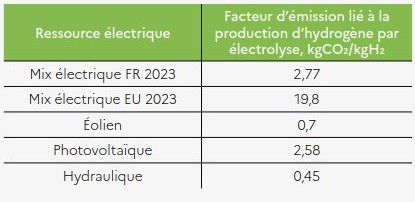
\includegraphics[width=1\linewidth]{image/chap1/facteur_emission_prod_H2_electrolyse.jpg}
\captionof{figure}{Facteur d'émission de la production d'hydrogène par électrolyse en fonction de la source d'électricité \cite{ADEME_2022}}
\label{fig: 1}
\end{center}

\end{multicols}

L’utilisation de l’hydrogène sous sa forme liquide n’est pas encore très répandue, elle demande des technologies encore peu développées. Elle est restreinte à des niches comme l’aérospatial qui concentre 34\% de la production de LH2, et à l’électronique (30\%), surtout en Amérique du nord (80\% de la consommation mondiale) selon l'International Energy Agency (IEA). 


\subsection{Les objectifs de la France et de l'Europe en 2030 et 2050}
\begin{multicols}{2}

\begin{center}
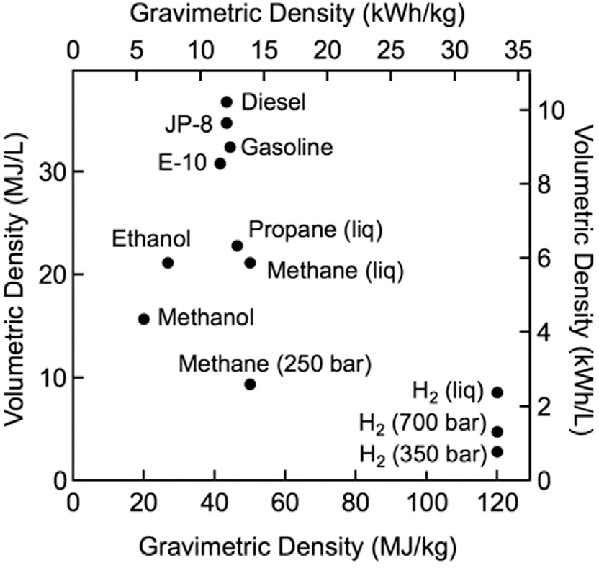
\includegraphics[width=.8\linewidth]{image/chap1/e-Comparison-of-gravimetric-density-and-volumetric-density-of-several-fuels-depending-on.PNG}
\captionof{figure}{Comparaison des densités massiques et volumiques de différentes espèces chimiques \cite{unkown1} }
\label{fig: density}
\end{center}

L’hydrogène liquide présente un fort potentiel de croissance dans les années qui viennent. Son intérêt majeur vient de sa densité énergétique. En effet pour un même contenu énergétique, l’hydrogène liquide est deux fois plus dense que l’hydrogène gazeux à haute pression (700 bars), ce qui permet de stocker et de transporter des volumes plus importants d’hydrogène dans les mêmes volumes. Les densités énergétiques de différents combustibles sont présentés en \ref{fig: density}.

\end{multicols}

Les objectifs de la transition énergétique française ou européenne sont déterminés par diverses organisations, qu'elles soient non-gouvernementales comme le GIEC (Groupe d'experts Intergouvernemental sur l'Evolution du Climat), ou gouvernementales comme l'Union Européenne.

Au niveau de l’UE et en réponse à la guerre en Ukraine, le projet REPowerEU prévoit de produire des énergies renouvelables, de produire 10 millions de tonnes d’$H_2$ renouvelable et d’en importer 10 millions d’ici 2030. De plus, l’UE souhaite déployer 40 GW de capacité d’électrolyse d’ici là. 

En France, France Hydrogène propose deux scénarios pour le développement d’hydrogène décarboné en France : Ambition 2030 qui consiste à utiliser 680 kt/an et un scénario ambitieux, Ambition 30+ qui consiste à utiliser 1090 kt/an. L'association souhaite favoriser trois secteurs : l’industrie, la mobilité et l’énergie. D’ici 2050, la stratégie française hydrogène prévoit l’installation d’une capacité de 6.5GW d’électrolyseurs. Un budget de 7.2 milliards d'euros a été consacré à cette stratégie et en octobre 2021, Emmanuel Macron a présenté France 2030, un plan d’investissement s’élevant à 30 milliards d’euros sur 5 ans et visant à faire de la France le leader de l’hydrogène vert en 2030. \\

\begin{figure}[h]
\centering
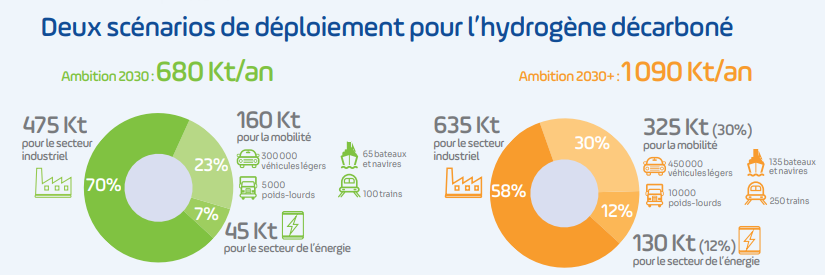
\includegraphics[width=.9\linewidth]{image/chap1/ambitions_scenarios.PNG}
\caption{Détail des deux scénarios de France Hydrogène \cite{hydrogene_2021}}
\end{figure}

\subsection{Les chaines de procédés}

Aujourd’hui, la plupart de l’hydrogène est produit par vaporeformage du méthane, ou Steam Methane Reforming en anglais (SMR), ce qui est coûteux en émission carbone. Pour décarboner la synthèse de l’hydrogène, on envisage d’installer des techniques de captage de CO2 sur le procédé de vaporeformage et de développer l’électrolyse, en utilisant de l’électricité décarbonée. On envisage d’installer 6,5 GW d’électrolyseurs en France et 850 GW dans le monde d’ici 2030 pour atteindre la neutralité carbone en 2050 (IEA). 
Nous détaillons donc ces deux méthodes de production de l’hydrogène dans notre étude. 

Le développement à grande échelle de l’hydrogène nécessite d’installer des infrastructures de stockage et de distribution. Premièrement, l’hydrogène est stocké dans des réservoirs. Pour des raisons d’encombrement, il est pressurisé ou liquéfié. Ces réservoirs peuvent être enterrés, semi-enterrés ou aériens. Les réservoirs enterrés présentent de nombreux avantages : ils occupent moins de place au sol, ont une plus grande capacité de stockage et sont plus sécurisés. Nous avons alors choisi de dimensionner uniquement le stockage enterré par la suite. Nous nous sommes intéressés à trois types de cavités : les cavités salines, les cavités minées non revêtues pour le stockage gazeux et les cavités minées revêtues pour le stockage liquide. 

Ensuite, il faut des infrastructures pour l’approvisionnement des véhicules. France Hydrogène prévoit d’augmenter le nombre de stations en service en France en passant de 57 en 2021, à 400 en 2025 puis entre 1000 et 1700, suivant le scénario envisagé, en 2030. La France pourrait importer de l’hydrogène depuis l’Ukraine, le Maghreb, le Moyen-Orient ou l’Amérique du Sud, ces derniers présentant des conditions favorables au développement d’énergies renouvelables. Il faudrait développer des pipelines entre pays frontaliers et au sein des pays, en parallèle du développement d’un réseau de camions, de bateaux ou de trains pour le transport.

Quels que soient les scénarios envisagés par l’ADEME, une grande part de l’hydrogène est utilisée dans l’industrie, que ce soit dans les raffineries, la production d’engrais (synthèse de l’ammoniac), l’industrie chimique ou l’acier. Un autre secteur prometteur est le domaine des transports. Nous n’avons considéré que l’industrie et les mobilités par la suite.\\

\subsection{Nos configurations}

Les configurations retenues s’ancrent dans deux thématiques : alimenter les industries ou les mobilités (Power to Mobility (P2M)/ Power to Industry (P2I)), et ont pour but de comparer les différents modes de production, la forme de l'hydrogène stocké et le type de stockage. \\
 
\textbf{Configuration 1 : Power to Mobility } \\
Alimentation de l’aéroport Charles de Gaulle et stockage en cavité saline. On se propose ici d’alimenter toute l’infrastructure de l’ensemble de l’aéroport à l’hydrogène. Cela ne concerne pas le carburant des avions. L’hydrogène serait produit par électrolyse et stocké en phase gazeuse en cavité saline . La consommation journalière de l’aéroport en H2 serait selon une estimation donnée par Air Liquide de 300 t par jour, avec 12h d’injection et 12h de soutirage. \\
 
\textbf{Configuration 2 :  Power to Mobility } \\
Stockage gazeux en cavité minée de l’hydrogène pour alimenter les mobilités (taxis, bus, voitures). Ici on stocke 230t d’$H_2$ par jour avec 12h d’injection et 12h de soutirage. \\
 
\textbf{Configuration 3 :  Power to Industry } \\
Alimentation d’un pôle industriel en hydrogène. Stockage gazeux dans une cavité saline selon le modèle de Spindletop au Texas d'Air Liquide (backup). On injecte pendant 5 mois pour soutirer pendant 1 mois 6400 t d’$H_2$. L’hydrogène serait produit par SMR avec captage de $CO_2$. \\

\textbf{Configuration 4 : Power to Industry }\\
Alimentation de toutes les infrastructures du port de Marseille-Fos. C’est un projet qui aura lieu entre 2026 et 2031 et qui vise à décarboner l’activité industrielle du port de Marseille-Fos. L’hydrogène serait produit par SMR avec captage de $CO_2$, puis stocké en phase gazeuse en cavité minée. La période d’injection serait de 3 semaines pour 1 semaine de soutirage. La masse d’hydrogène utile serait de 1000 t. \\

\textbf{Configuration 5 :  Power to Mobility }\\
Production d'hydrogène par électrolyse et stockage sous forme liquide dans un réservoir enterré de 73$m^3$. Ce réservoir d’une capacité de 5,2 t constituerait une station pour alimenter les véhicules à hydrogène, avec vaporisation au préalable. \\

\textbf{Configuration 6 : Power to Mobility}\\
Production d'hydrogène par électrolyse et stockage sous forme liquide dans des cavités minées revêtues afin d’alimenter un réseau de transport à hydrogène. La demande en hydrogène est de 230 t par jour.  \\

\textbf{Configuration 7 : Power to Industry. }\\
Stockage de l'hydrogène sous forme liquide en cavité minée revêtue. Cette configuration est analogue à celle du port de Marseille puisqu’elle vise à comparer l’efficacité du stockage sous forme liquide et gazeuse. Les durées de soutirage et la masse utile (1000 t) sont les mêmes que pour le scénario de Marseille-Fos.\\

Les schémas de chacune des configurations seront présentés en annexe A. Ils permettent de visualiser plus directement les différents usages et applications.











\section{Chapitre II : Le stockage souterrain d'hydrogène}
Un des intérêts premiers de l'hydrogène est sa capacité, une fois produit, d'être stocké sans pertes énergétiques, au contraire des batteries stockant de l'électricité qui se déchargent au cours du temps. En tirant partie de cette propriété de l'hydrogène, nous caractérisons donc des réservoirs pour celui-ci. 

Ceux-ci seront enterrés: la pression des roches entourant les stockages permet d'utiliser moins de matériaux de construction. De plus grandes quantités d'hydrogène peuvent ainsi y être conservées.

Il existe différentes techniques de stockage en fonction de la géologie du terrain. Dans le sous-sol, à des profondeurs très variables, on constate la présence de couches de sel sur plusieurs centaines de mètres d'épaisseur. Ce sont les vestiges d'anciennes mers intérieures qui se sont évaporées. Ces roches salines sont une aubaine : le sel étant à la fois étanche aux gaz et soluble dans l'eau, le stockage de gaz et la création de cavité est grandement facilité (voir sous-section création de cavité). C'est une technique de stockage très répandue pour le gaz naturel. On peut notamment citer les stockages de gaz naturel de \emph{Storengy}, filliale d'\emph{Engie} à Etrez dans l'Ain. Lorsqu'il n'y a pas de couches de sel, on est contraint de creuser la roche pour créer des cavités en utilisant des techniques minières et en mettant en place un revêtement pour assurer l'étanchéité. On parle alors de stockage en cavité minée revêtue.


\subsection{Dimensionnement preliminaires des stockages}
Nous détaillons ici les techniques de dimensionnement de différentes configurations.
\subsubsection{Configuration de cavité saline}
La cavité saline est envisagée uniquement pour le stockage de l'hydrogène en phase gazeuse. Nous cherchons à déterminer la pression dans la cavité et son volume. Prenons comme exemple la première configuration. On injecte l’H2 dans la cavité pendant 12h puis on le soutire pendant les 12h restantes. Le débit d’injection (respectivement soutirage) serait alors donné par $$ D_{injection}=\frac{m_{H_2}}{T_{injection}} \ \ \  D_{soutirage}=\frac{m_{H_2}}{T_{soutirage}} $$

\begin{multicols}{2}
Initialement, le massif est soumis à un régime de contraintes initiales dans trois directions (cf. figure ~\ref{fig:chap2contrainteSaline}) La contrainte verticale est donnée par le poids des terrains : $$\sigma_\nu = \rho g H $$ avec $\rho$ la masse volumique du sol, $g=10 m.s^{-2} $ l'accélération de pensanteur et $H$ la profondeur.
 
\begin{center}
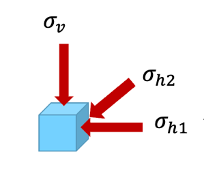
\includegraphics[width=.4\linewidth]{image/chap2/cube_contraintes.png}
\captionof{figure}{Représentation des contraintes}
\label{fig:chap2contrainteSaline}
\end{center}

\end{multicols}

Pour simplifier on considère que les deux contraintes horizontales initiales sont égales à la contrainte verticale $\sigma_\nu = \sigma_{h1} = \sigma_{h2} $. Ensuite on prend un coefficient de sécurité pour les pressions maximales et minimales : une pression trop élevée peut causer des fractures dans le sel, endommageant l’étanchéité de celui-ci et une pression trop basse peut faire que la cavité se referme sur elle-même. Ainsi: \ $P_{max} \le 0,8 \sigma_{\nu}$ et $ P_{min} \ge 0,2 \sigma_{\nu} $

En considérant que l'hydrogène est un gaz parfait, on peut calculer le volume de la cavité comme suit : $$ V_{cav} = \frac{m_{utile} R T }{ M(H_2) \Delta P} $$ On définit la masse d'hydrogène coussin comme la masse d'hydrogène pour la pression minimale et on déduit la masse utile : $$ m_{utile} = m_{totale} - m_{coussin} $$

Reste à dimensionner les puissances électriques nécessaires à ce type d'installation. La puissance de l'électrolyseur doit être de $P_{elec} = PCI \times D_m $ où le pouvoir calorifique inférieur de l’hydrogène ($PCI$) est de $121 000 MJ/kg$. Sachant que les électrolyseurs ont un rendement de 0.62, la puissance électrique nécessaire est de $P=\frac{P_{elec}}{0.62}$. L'ensemble des résultats sont disponibles en Annexe B.

\subsubsection{Configuration de cavité minée revêtue}
On s'intéresse aux cavités minées revêtues, dans un premier temps pour stocker du gaz, et ensuite du liquide. Les tableaux de données sont aussi disponibles en Annexe B.
Pour le stockage gazeux, les pressions minimales et maximales sont fixées par l'opérateur et le revêtement mis en place permet de les supporter. Le volume de la cavité est ainsi calculé comme précédemment par rapport à ces deux pressions. Concernant la détermination de la profondeur, la méthode du cône rigide est utilisée.
Il faut équilibrer les forces de pression du gaz sur la cavité $F_{LRC}$ (Lined Rock Cavern, Cavité minée revêtue) et le poids $W$ des roches surplombant celle-ci, comme on peut le voir sur la figure ~\ref{fig:chap2schemaContrainteMinee}. On a $$F_{LRC}=\pi r^2 \rho \ \ , \ \ W =\rho g \pi [r^2 d + (r d^2 tan(\alpha)) + \frac{1}{3} d^3 tan^2(\alpha)]$$

\begin{figure}[h!]
\centering
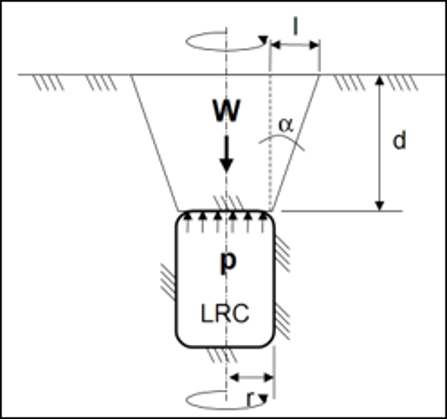
\includegraphics[width=0.4\linewidth]{image/chap2/schema_poids_cavite_minee.png}
\caption{Cavitée minée et représentation des forces.}
\label{fig:chap2schemaContrainteMinee}
\end{figure}

On note donc $FS= W/F_{LRC} $ le facteur de sécurité. La figure ~\ref{fig:chap2graphFS} le montre à différentes pressions en fonction de la profondeur: 

\begin{figure}[!h]
\centering
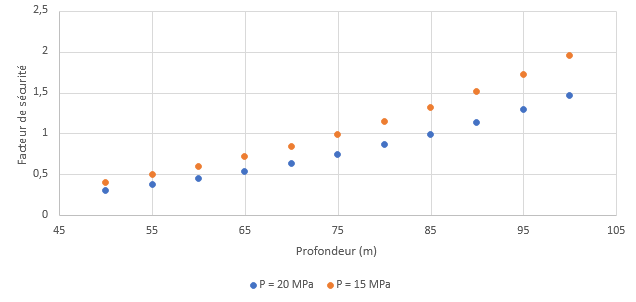
\includegraphics[width=.8\linewidth]{image/chap2/courbe_facteurDeSecu.png}
\caption{Facteur de sécurité en fonction de la profondeur aux pressions de 20 MPa et 15MPa.}
\label{fig:chap2graphFS}
\end{figure}

Le facteur de sécurité étant jugé suffisant à partir de 1,5 on choisit une pression de 20 MPa pour une profondeur de 100m (on a fixé $\alpha = 40\textrm{°}$ et on a pris un rayon de 15m).\\

\subsubsection{Configurations du stockage liquide}
L’hydrogène ne peut exister sous forme liquide qu'à des températures extrêmement basses (de l’ordre de -253°C). Cependant, aucune forme de stockage n’est capable de maintenir l’hydrogène à cette température : celui-ci se réchauffe, ce qui entraîne l’évaporation d’une partie du stock et l’augmentation de la pression dans le réservoir, c’est le phénomène de boil-off.

Si l’on néglige ce boil-off, le stockage de l’hydrogène sous forme liquide est relativement simple à dimensionner ; en effet, sa densité liquide est quasiment constante.
De plus les conditions de pression étant plus favorables, on peut stocker le LH2 en surface, dans des réservoirs enterrés à de très faibles profondeurs ou dans des cavités minées revêtues.

Il y a deux approches de dimensionnement du stockage liquide. La première est de reprendre les scénarios précédents de stockage gazeux et de calculer la quantité d’hydrogène liquide que l’on peut stocker dans une cavité de même dimension. La seconde approche consiste à dimensionner une nouvelle cavité plus petite et directement adaptée à l’usage considéré. Cette seconde approche a été retenue.

On peut également considérer le stockage dans un réservoir enterré dont les dimensions sont données en annexe C. On peut donc calculer le volume du réservoir cylindrique ($73 m^3$) et, connaissant la masse volumique de l’hydrogène liquide ($71 kg/m^3$), on en déduit que le réservoir stocke 5,2 tonnes d’hydrogène. De tels réservoirs seraient adaptés à la configuration 5.



\subsection{Rhéologie des roches}

Lors du dimensionnement d’une cavité (saline ou minée), il est important de connaître les caractéristiques thermomécaniques des roches dans lesquelles la cavité sera créée. Pour ce faire, des échantillons sous forme de carottes sont prélevés dans le site considéré et envoyés dans un laboratoire spécialisé pour réaliser des essais géomécaniques. 
 
Outre la mesure des propriétés physiques (masse volumique et vitesse du son qui caractérise la continuité du matériau) et des propriétés thermiques (conductivité, capacité volumique, coefficient de dilatation), la caractérisation de la roche au laboratoire comprend divers types d’essais (essais brésiliens, de compression simple et triaxiale, de cisaillement) dont le détail est donné en Annexe D.
 
Aussi, le sel étant un matériau viscoplastique, il convient de réaliser des essais de fluage. En effet, si on applique une contrainte constante à notre éprouvette de sel, sa déformation va dépendre du temps.  
On effectue donc un essai triaxial durant quelques mois pour mesurer la déformation relative de l’échantillon au cours de l’expérience sous différents paliers de déviateur de contraintes et de température.

Plusieurs lois permettent de caractériser cette déformation, mais nous avons choisi d’utiliser la loi puissance de Lemaitre. En somme, au cours d'un essai de fluage, la déformation axiale totale de l'éprouvette est la somme d’une déformation élastique, d'une déformation viscoplastique irréversible donnée par la loi de Lemaitre, et d'une déformation de dilatation thermique.

$$ \epsilon = \frac{q}{E} + (\frac{q}{K})^{\beta} exp(A[\frac{1}{T_{ref}} - \frac{1}{T}])t^{\alpha} + a_{th} (T-T_0) $$
Avec : \begin{itemize}
\item $q$ le déviateur de contraintes
\item $E$ le module d'\emph{Young}
\item $\alpha$,$\beta$, $K$ les paramètres de la loi de \emph{Lemaitre}
\item $ A $ le coefficient de la loi d'\emph{Arhénius}
\item $T, T_0$ et $T_{ref}$ les température, température initiale et température de référence
\item $t$ le temps
\item $a_{th} $ le coefficient de dilatation thermique linéaire.
\end{itemize}
Les résultats des essais de fluage sont ajustés grâce à une méthode des moindres carrés pour déterminer les paramètres de la loi de Lemaitre ($\alpha,\beta, K, A$) ainsi que le coefficient de dilatation thermique $a_{th}$. 


\subsection{Simulations numériques des cavités}

Le but est maintenant de confirmer la fiabilité du dimensionnement préliminaire défini ci-dessus en modélisant les différentes cavités. Pour cela, nous avons simulé les propriétés thermomécaniques des cavités à l’aide du logiciel \emph{DEMETHER} (des extraits de la notice sont donnés en annexe E) et nous avons vérifié la stabilité des stockages. Nous avons également adapté le dimensionnement aux résultats.

\subsubsection{Des cavités pour GH\textsubscript{2}}
Pour pouvoir faire les simulations des cavités de stockage, il faut tout d’abord s’intéresser à la théorie de la modélisation et au fonctionnement du logiciel utilisé. \\

\textbf{A-Théorie des modélisations}\\

Afin de vérifier la stabilité des cavités, la simulation du comportement des cavités prend en compte les propriétés thermomécaniques des roches. Une cavité est définie par plusieurs critères :
\begin{itemize}
\item Les pressions minimale et maximale doivent être respectées.
\item Il ne doit pas y avoir de contrainte de traction.
\item Il ne doit pas y avoir de dilatance de la roche (seulement dans le cas du sel).
\item La perte de volume de la cavité doit être inférieure à 1\% par an.
\end{itemize}
Sans ces critères, il y a un risque d’instabilité des cavités ou de fuite d’hydrogène.

\begin{multicols}{2}


\begin{center}
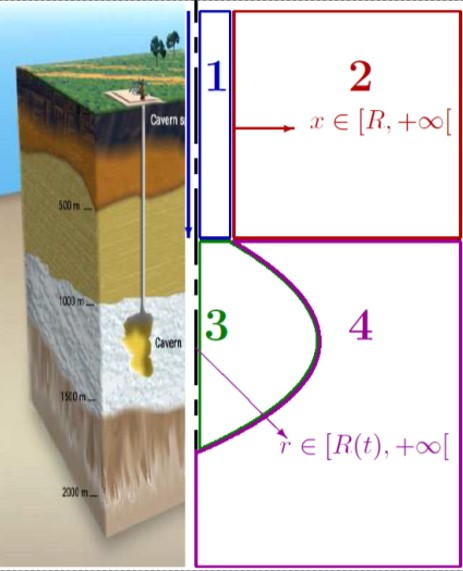
\includegraphics[width=.9\linewidth]{image/chap2/schema_cav.jpg}
\captionof{figure}{Découpage typique d'une cavité}
\end{center}

Le logiciel \emph{DEMETHER} que nous avons utilisé nous a permis de vérifier la stabilité des cavités. Le logiciel découpe la zone de stockage en 4 parties : 
\begin{enumerate}
\item Le puits
\item Le massif autour du puits
\item Le massif autour de la cavité
\item La cavité
\end{enumerate}
Il permet de simuler le lessivage de la cavité, le remplissage avec de l'hydrogène, le cyclage et le comportement à long terme.

Le logiciel s'intéresse à différents phénomènes : 
\begin{itemize}
\item Le puits est simulé en 1D et découpé en 2 espaces (central et annulaire). On s’intéresse spécifiquement à l’écoulement du fluide (densité, vitesse d’écoulement, température).
\item La simulation du massif autour du puits prend surtout en compte la conduction thermique (température).
\item Au niveau du massif de la cavité, on s’intéresse à la conduction et aux réactions mécaniques (température et contraintes).
\item Dans la cavité, il s’agit de s’intéresser aux états thermodynamiques des différents fluides présents (température, pression, conductivité thermique).
\end{itemize}

\end{multicols}

 
Les principales équations thermomécaniques utilisées sont présentées ci-dessous: l'équation d'équilibre, l'équation de la chaleur et la loi de Fourier.  
 $$
 	\vec{\nabla}\sigma + \rho \vec{g} = \vec{0} \ \ , \ \
	\rho C \frac{\partial T}{\partial t} + div(\vec{j}) = S \ \ , \ \
	\vec{j} = - \lambda \vec{\nabla}T
 $$
Avec:
\begin{itemize}
\item $\sigma$ le tenseur des contraintes de Cauchy
\item $\vec{g}$ l'accélération de pensanteur
\item $\rho$ la masse volumique
\item $C$ la capacité thermique 
\item $T$ la température
\item $\vec{j}$  la densité de courant de chaleur et $\lambda$ la conductivité thermique
\item $S$ le terme source
\end{itemize}

Pour les cavités salines, il est également nécessaire de prendre en compte le fluage du sel, décrit par la loi de Lemaitre. Contrairement au dimensionnement préliminaire, qui considère l'hydrogène comme un gaz parfait, la modélisation cette fois-ci rend compte des vraies lois d'état, notamment l'effet Joule-Thomson. 

\emph{DEMETHER} va alors résoudre l’ensemble des équations thermodynamiques et thermomécaniques pendant les différentes phases dans les zones voulues. Nous nous sommes surtout intéressés aux zones 3 et 4, qui sont les plus importantes pour notre étude. \\

\textbf{B-Application aux cavités salines}\\

On a simulé grâce au logiciel \emph{DEMETHER} le comportement du stockage de l'hydrogène gazeux en cavité saline pendant une durée de plus de trente ans (ce qui correspond environ à la durée de vie d’une cavité). La modélisation commence par le lessivage (technique pour creuser la cavité), puis on remplit la cavité et finalement on simule 30 ans de cycle. On a ainsi étudié deux situations : le cas où le stockage est destiné à l’industrie, et le cas où il est destiné à la mobilité (cf. Annexe E).

Dans la première application relative à l'industrie (configuration 3), nous considérons 1095 jours de lessivage à $P = P_{saumure} = 11,7 MPa$, 180 jours de remplissage (où la pression augmente jusqu’à $P = 14,5 MPa$) et 30 ans de cyclage. Nos résultats ont confirmé que la cavité saline envisagée était bien réalisable. En effet, nos modélisations donnent des pressions minimale et maximale admissibles par rapport aux seuils de stabilité, des contraintes négatives (ce qui confirme qu'il s'agit bien d'une compression et non d'une traction), des pertes volumiques en dessous de 1\% par an et un déviateur $q(p)$ de contrainte toujours inférieur au critère de dilatance linéaire considéré ($q = 1,3 p + 2,5$) où $p$ est la pression moyenne. Les figures 8 et 9 illustrent le résultat obtenu pour la configuration 3.\\

\begin{figure}[h!]
\centering

\begin{subfigure}[b]{0.4\linewidth}
    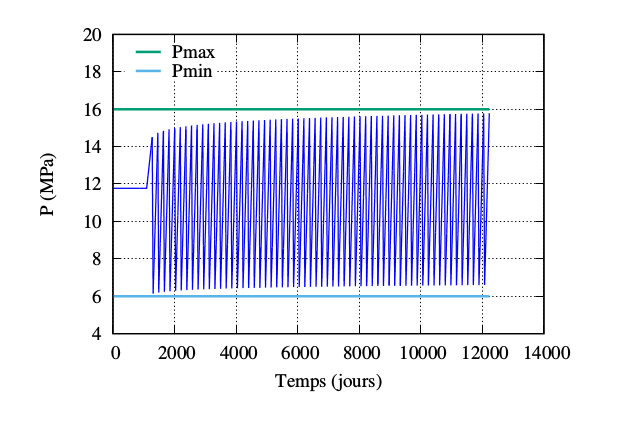
\includegraphics[width=\linewidth]{image/chap2/P1.png}
    \caption{Evolution de la pression (MPa).}
\end{subfigure}
\hspace{1cm}
\begin{subfigure}[b]{0.4\linewidth}
    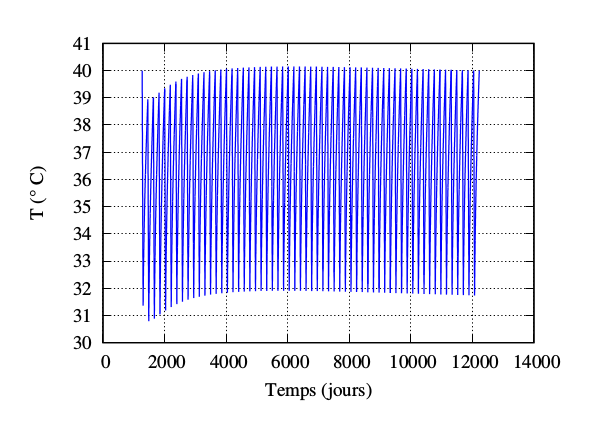
\includegraphics[width=\linewidth]{image/chap2/T1.png}
    \caption{température (ºC).}
\end{subfigure}

\begin{subfigure}[b]{0.42\linewidth}
    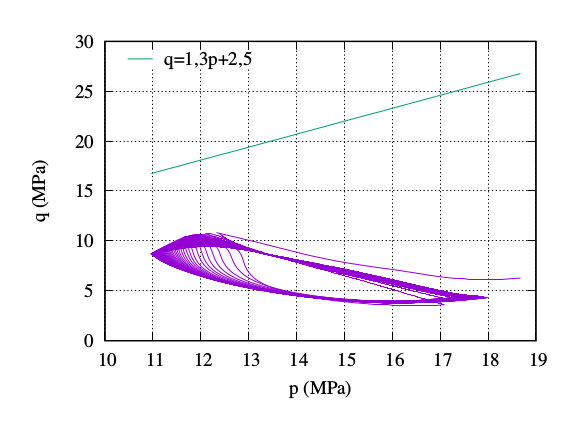
\includegraphics[width=\linewidth]{image/chap2/q(t)1.png}
    \caption{déviateurs (MPa).}
\end{subfigure}
\begin{subfigure}[b]{0.42\linewidth}
    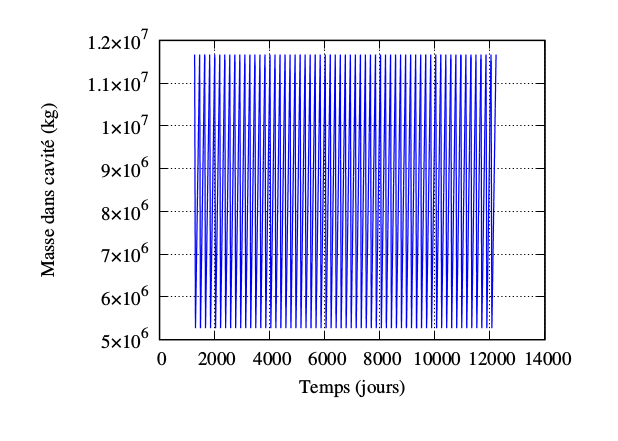
\includegraphics[width=\linewidth]{image/chap2/M1.png}
    \caption{masse (kg).}
\end{subfigure}

\caption{Evolution de la pression (MPa), température (ºC), déviateurs (MPa), masse (kg)}

\end{figure}

\begin{figure}[h!]
\centering

\begin{subfigure}[b]{0.3\linewidth}
    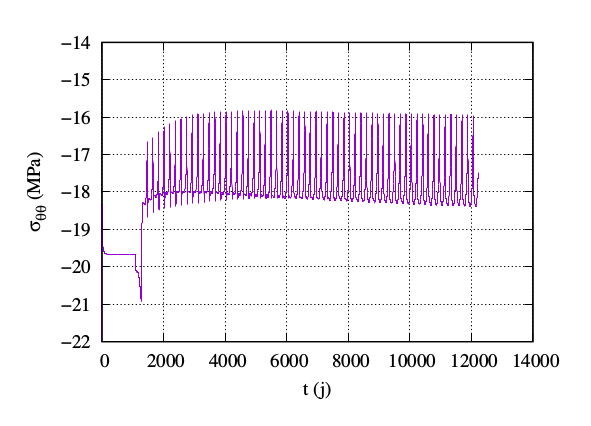
\includegraphics[width=\linewidth]{image/chap2/STT1.png}
    \caption{contrainte orthoradiale (MPa).}
\end{subfigure}
\hspace{0.1cm}
\begin{subfigure}[b]{0.3\linewidth}
    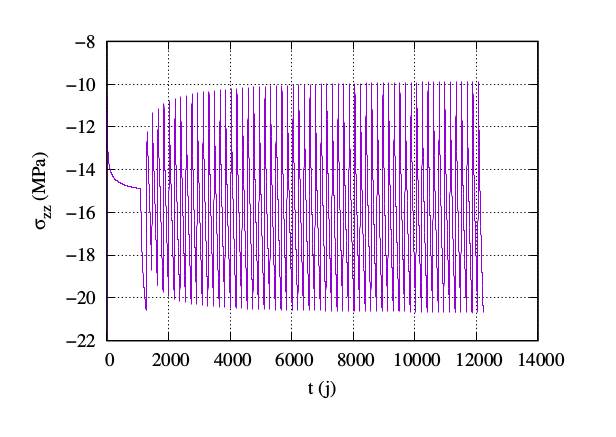
\includegraphics[width=\linewidth]{image/chap2/SZZ1.png}
    \caption{contrainte selon z (MPa)}
\end{subfigure}
\hspace{0.1cm}
\begin{subfigure}[b]{0.3\linewidth}
    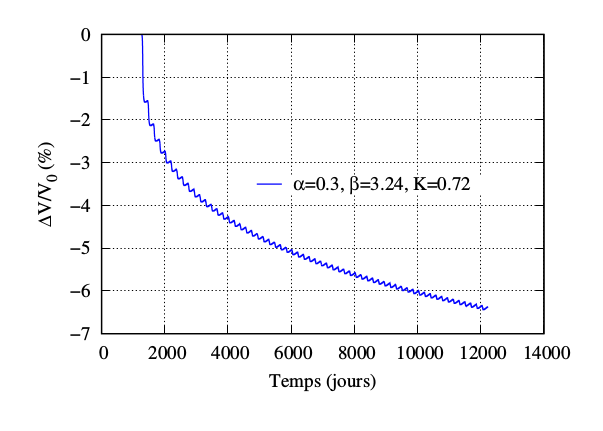
\includegraphics[width=\linewidth]{image/chap2/Volume1.png}
    \caption{variation volumique (\%).}
\end{subfigure}

\caption{Evolution de la  contrainte orthoradiale (MPa), contrainte selon z (MPa) et variation volumique (\%) au cours du temps dans la cavité}
\label{fig:7 figures}
\end{figure}



\textbf{C-Applications aux cavités minées revêtues}\\

Nous avons également utilisé le logiciel \emph{DEMETHER} dans le but de simuler la création, le remplissage et les cycles soutirage-injection des cavités minées non revêtues (le logiciel ne permettant pas de modéliser l’intéraction entre revêtement et le gaz/les roches).

Contrairement au sel, les roches n’ont pas un comportement visco-plastique mais uniquement élastique, il n’y a pas de phénomène de fluage. Nous avons pris en entrée cinq paramètres pour décrire les propriétés thermodynamiques des roches résistantes qui entourent la cavité : deux propriétés mécaniques et trois propriétés thermiques résumées dans le tableau ci-dessous:\\


\begin{table}[h]
\centering
\begin{tabular}{|l|l|}
\hline
Module D'Young ($Pa$) & $2,5\times 10^{10}$ \\
\hline
Coefficient de Poisson & $0,25$ \\
\hline
Conductivité thermique ($W.m^{-1}.K^{-1})$ & $0,22$ \\
\hline
Diffusivité thermique ($m^2.s^{-1}$) & $0,08265$ \\
\hline
Coefficient de dilatation thermique ($K^{-1}$) & $5\times 10^{-1}$ \\
\hline
\end{tabular}
\caption{Donnnées thermomécaniques des roches compétentes}
\end{table}

Le revêtement assurant l'étanchéité du stockage supportant les contraintes de traction développées n'étant pas pris en compte dans la modélisation, le critère d'analyse considéré s'est focalisé surtout sur les variations de température pour éviter des valeurs négatives conduisant à la congélation des roches.\\

Nous avons simulé des cavités cylindriques contenant de l'hydrogène gazeux avec les débits d’injection et de soutirage issus du dimensionnement préliminaire. Les simulations ont permis de montrer que les dimensionnements préliminaires conduisaient à des cavités instables. La solution était alors de créer plusieurs cavités plus petites. Les caractéristiques des cavités pour les applications de l'hydrogène à la mobilité et à l'industrie sont données dans la table 2.

\begin{table}[h]
\centering
\begin{tabular}{|c||c|c|c|c|c|}
\hline
Application & Profondeur (m) & Nombre de cavités & Hauteur (m) &  Rayon (m) & Volume ($m^{3}$) \\
\hline
Industrie & 100 & 3 & 45 & 15 &  32 000 \\
\hline
Mobilité & 100 & 2 & 30 & 15 & 22 000 \\
\hline
\end{tabular}
\caption{Propriétés des stockages en cavités minées revêtues}
\end{table}


Regardons les résultats obtenus pour une application industrielle du stockage de l’hydrogène gazeux (les résultats pour une application à la mobilité sont donnés en annexe E). 

\begin{figure}[h]
\centering
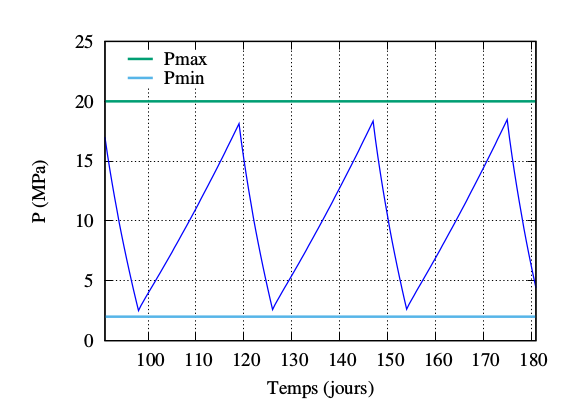
\includegraphics[width=0.5\linewidth]{image/chap2/Cavité minée GH2 P2I pression au cours du temps.png}
\caption{Evolution de la pression dans la cavité au cours du temps sur trois cycles}
\label{fig:pression}
\end{figure}


\begin{figure}[h!]
  \centering
  \begin{subfigure}[b]{0.43\linewidth}
    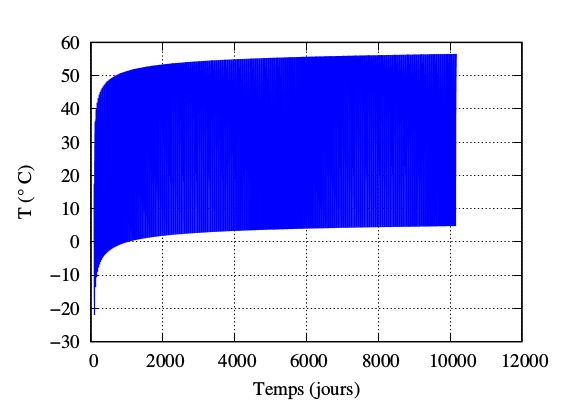
\includegraphics[width=\linewidth]{image/chap2/Cavité minée GH2 P2I température au cours du temps 40°C.png}
    \caption{Température d’injection de 40 °C.}
  \end{subfigure}
  \begin{subfigure}[b]{0.4\linewidth}
    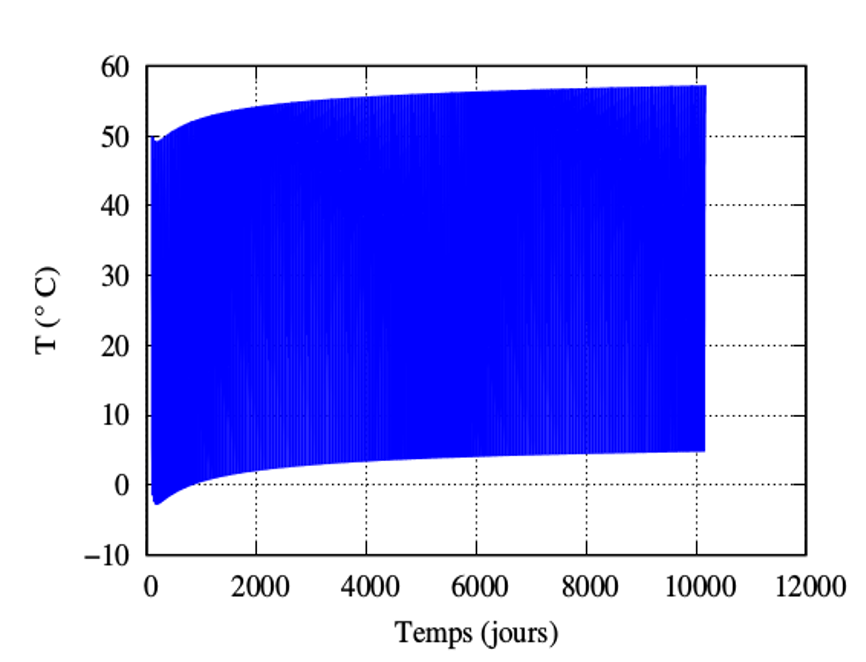
\includegraphics[width=\linewidth]{image/chap2/Cavité minée GH2 P2I température au cours temps 50°C.png}
    \caption{Température d'injection de 50 °C.}
  \end{subfigure}
  \caption{Evolution de la température au cours du temps dans la cavité}
  \label{fig:température}
\end{figure}

On constate que les roches subissent des écarts de température d’environ 50 °C. La température lors du soutirage devient négative. Cette diminution de température dans la cavité vient du fait que le gaz se détend. C’est pourquoi nous avons augmenté la température d’injection de l’hydrogène de 10 °C lors d’une deuxième simulation. \\

On simule enfin les contraintes dans la cavité. 

\begin{figure}[h!]
  \centering
  \begin{subfigure}[b]{0.4\linewidth}
    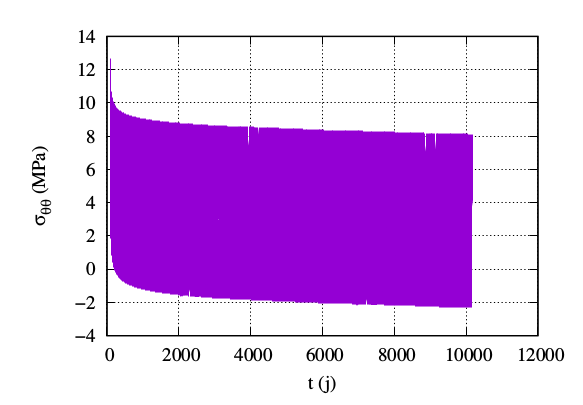
\includegraphics[width=\linewidth]{image/chap2/Cavité minée GH2 P2I contrainte teta teta au cours temps.png}
    \caption{Composante orthoradiale.}
  \end{subfigure}
  \begin{subfigure}[b]{0.43\linewidth}
    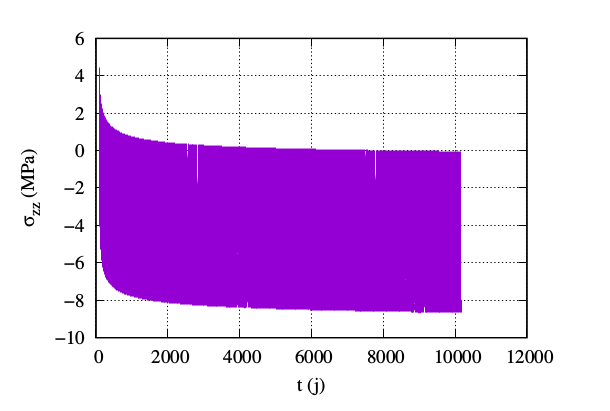
\includegraphics[width=\linewidth]{image/chap2/Cavité minée GH2 P2I contrainte zz au cours temps.png}
    \caption{Composante verticale.}
  \end{subfigure}
  \caption{Evolution de la contrainte pour la cavité cylindrique au cours du temps}
  \label{fig:contrainte}
\end{figure}

Les contraintes sur la figure 12 prennent des valeurs positives. Les roches entourant la cavité entrent donc en traction, ce qui justifie la nécessité d’un revêtement. Les caractéristiques du revêtement à mettre en place sont décrites dans la section 2.4.2 ci-dessous consacrée à la création des cavités minées revêtues.



\subsubsection{Des cavités pour LH\textsubscript{2}}
On distingue les reservoirs enterrés et les cavités minées revêtues.\\

\textbf{A-Réservoirs enterrés}\\
Afin d’augmenter sa densité énergétique, l'hydrogène peut être stocké sous forme liquide. Nous allons ici nous intéresser au stockage dans des réservoirs enterrés. Le réservoir est une cuve cylindrique (cf. annexe C figure 48) enfoui à quelques mètres de profondeur constitué de dalles de béton, de sable, d’un isolant et de deux coques en acier. Les dimensions sont données dans l'Annexe C sur la figure 47.

Compte tenu de la température de l’hydrogène liquide dans le réservoir ($T = 20K$), le froid risque de se propager dans le sol entourant la cuve et l’eau qu’il contient peut geler. L’eau solide occupant un volume plus important que l’eau liquide, cela risquerait d’engendrer un phénomène de gonflement du sol. Afin d’éviter ce phénomène, nous avons mené une étude sur le logiciel \emph{COMSOL} pour suivre l’évolution de température dans le sol et en surface. Pour cela, nous allons dimensionner le type d'isolant, l'épaisseur de l'isolant et la profondeur d'enfouissement.\\

Nous avons travaillé sur un réservoir en 2D d’une part pour écourter les temps de calculs et d’autre part car l’étude en 2D est plus contraignante que celle en 3D : en effet on néglige les effets de bord en 2D, ce qui en réalité permet une meilleure évacuation de la chaleur. Nous avons pris également en compte le gradient de température dans le sol : on perd 3°C tous les 100m. Toutes les figures présentées en Annexe F sont prises au bout de 10 ans.  


Dans un premier temps, nous avons lancé la simulation pour une température extérieure constante de 17°C, deux types d’isolants (air et perlite) d’une épaisseur de 15 cm.  
Les résultats sont présentés en figure 72 de l'Annexe F. En réalité, la température dépend des saisons. Pour en tenir compte on suppose une température sous la forme : $$T_a(t) = A_a=B_a cos(\frac{2\pi(t-t_a)}{\tau})$$ $$A_a=\frac{1}{2}(T_{max} + T_{min}) \ , \ \ B_a =\frac{1}{2} ( T_{max} + T_{min})$$
Avec $T_{max}=25°C$,$T_{min}=5°C$ et $\tau=365 j$.


Les résultats obtenus montrent que l’air, même à 30 cm d’épaisseur ne constitue pas un très bon isolant. Pour la perlite, on peut descendre à 7cm sans que l’eau contenue dans le sol ne gèle. Pour que le dimensionnement puisse garantir l’isolation pour des conditions plus extrêmes de température (qui dépendent de l’endroit de creusement) et pour maintenir une marge de sécurité, on prend une épaisseur de 30cm.
Dans ce cas, même pour une température moyenne de 2°C, l’isolation est efficace alors que ce n’est pas le cas pour une épaisseur de 7 cm (cf. Annexe F) 

On peut maintenant jouer sur 3 autres paramètres: 
\begin{itemize}
\item La porosité du sol: plus un sol est poreux et plus le froid se propage loin (cf. Annexe F)
\item La profondeur: on voit que dans les deux cas, la répartition de température est assez semblable (cf. Annexe F). Pour des raisons économiques évidentes, on va donc se placer à une faible profondeur.
\item H, le coefficient d’échange avec le sol: on voit que lorsque les échanges thermiques avec la surface sont importants, le froid se propage vers le bas, et remonte moins en surface. (cf. Annexe F)
\end{itemize}

Ainsi en tenant compte de ces conditions, on retiendra pour notre isolant la perlite avec une épaisseur de 30cm et une faible profondeur du réservoir. \\

\textbf{B- Cavités minées revêtues}\\

\begin{multicols}{2}


Les cavités minées revêtues sont une autre alternative pertinente pour le stockage de l’hydrogène liquide. Elles peuvent être creusées à faible profondeur, puisqu’il n’y a aucune contrainte concernant la pression (question qui se pose lors du stockage d’hydrogène gazeux). Comme pour le réservoir enterré, il est nécessaire d’avoir un revêtement isolant (afin de conserver l’hydrogène à une température de 20 Kelvin, mais aussi pour garantir la stabilité des roches, qui peuvent supporter des températures allant jusqu’à – 80°C selon le rapport de Geostock \cite{Geostock_2022}), ainsi qu’étanche, pour éviter toute fuite d’hydrogène liquide.

Nous avons donc envisagé l’utilisation de cavités minées revêtues pour le scénario 7, en nous basant essentiellement sur l’étude de Geostock concernant le stockage de GNL (Gaz Naturel Liquéfié), ainsi que sur la cavité pilote réalisée à Daejon en Corée du Sud avec de l’azote liquide \cite{Nicolas_2008}. De fait, il n’existe pas encore de cavité minée revêtue pour le stockage d’hydrogène liquide (ni pour le GNL).

\begin{center}
  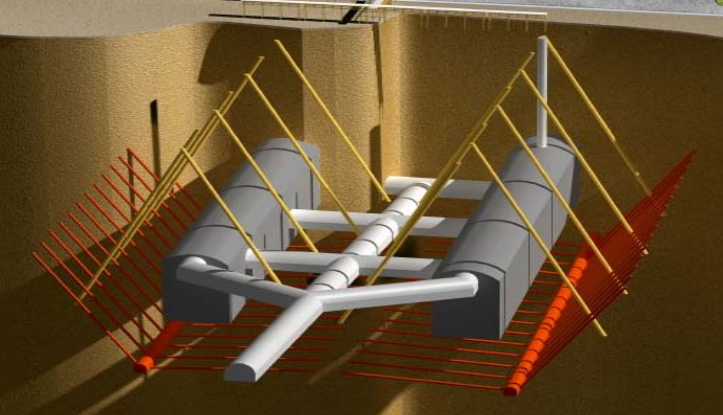
\includegraphics[width=\linewidth]{image/chap2/Figure 3.ii.2-1.png}
  \captionof{figure}{Structure des deux cavités minées revêtues du projet de Geostock pour le GNL}
\end{center}

Nous devions ainsi dimensionner la cavité afin qu’elle ait une capacité de 143 tonnes d’hydrogène, soit un volume total de 2014 $m^3$. Nous avons donc choisi de réaliser deux cavités de 1007 $m^3$ reliées par un réseau de galeries d’accès, comme pour le projet de Geostock [Figure 13].
Pour chaque cavité, nous avons conservé la forme des cavités standards (qui est régie par les panneaux d’acier utilisés pour le revêtement).\\

\end{multicols}


Nous nous sommes ensuite intéressés au revêtement de la cavité minée (cf. figure 14 a). Celui-ci est constitué de plusieurs épaisseurs. La première est un « pare-vapeur » permettant l’étanchéité de la cavité. Ensuite vient une couche de béton, puis une couche d’isolant (généralement de la mousse de polyuréthane) entre deux épaisseurs de contreplaqué (afin d’avoir une surface parfaitement plane), ce qui permet à la fois de maintenir l’hydrogène à 20K, mais aussi d’éviter les températures extrêmement froides dans les roches. Puis vient un panneau ondulé en acier inoxydable de faible épaisseur (1,2 mm).
Ce revêtement est inspiré de ceux utilisés dans les cuves des méthaniers transportant du gaz naturel liquéfié (cf. figure 15 b) qui sont également adaptés au transport d’un liquide devant être maintenu à très basse température (-160°C à pression atmosphérique).\\

\begin{figure}[h!]
\centering
\begin{subfigure}[b]{0.4\linewidth}
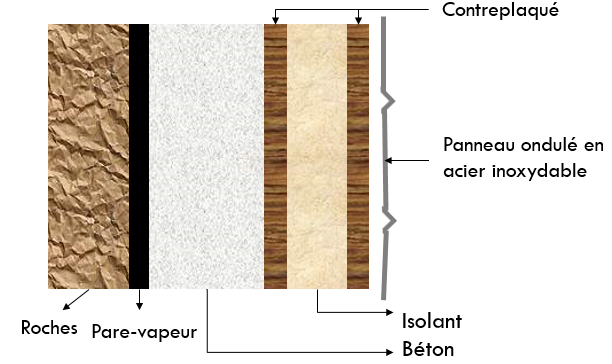
\includegraphics[width=\linewidth]{image/chap2/Figure 3.ii.2-3.png}
\caption{Structure du revêtement de la cavité}
\end{subfigure}
\begin{subfigure}[b]{0.4\linewidth}
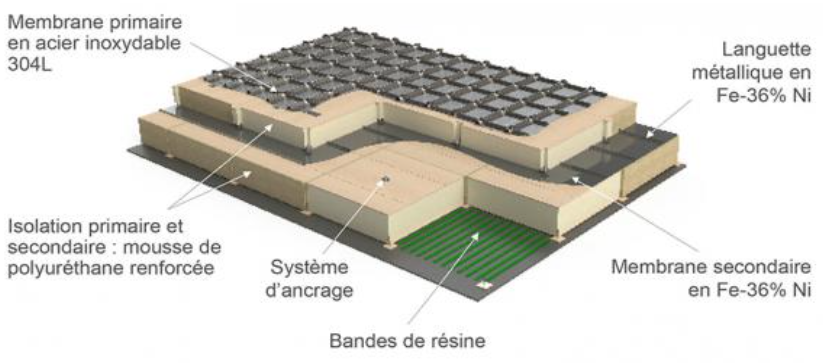
\includegraphics[width=\linewidth]{image/chap2/Figure 3.ii.2-4.png}
\caption{Structure du revêtement des cuves des méthaniers}
\end{subfigure}
\caption{Revêtments pour les cavitées minées revêtues}
\end{figure}

Ensuite, nous nous sommes intéressés au phénomène de formation de glace autour de la cavité. En effet, contrairement au cas du réservoir enterré, il n’est pas nécessaire ici d’éviter complètement la formation de glace, car la cavité est située à faible profondeur dans un massif exposé à l'eau (nappe, circulation dans des fractures...). De plus, la formation d’un anneau de glace autour de la cavité sert également de seconde barrière d’étanchéité (en empêchant l’eau de s’infiltrer mais également l’hydrogène liquide de s’échapper). Cependant, il est nécessaire de contrôler la formation de glace autour de la cavité, pour éviter une surpression contre le revêtement. Ainsi, pendant la création de la cavité, l’eau des roches environnantes doit être draînée. 

En s'appuyant sur les résultats de la modélisation du réservoir enterré, nous recommmandons le même type de revêtement que celui utilisé pour les expériences de stockage de GNL en cavités minées revêtues en remplacant toutefois l'isolant en polyuréthane par de la perlite sur un épaisseur de 40 cm.

Pour améliorer le dimensionnement, il faudrait effectuer des simulations à l’aide du logiciel \emph{COMSOL}, équivalente à celles menées sur le réservoir enterré.\\



\subsection{Réalisations des cavités}
Les techniques de création de cavités de stockage pour l'hydrogène dépendent de la nature géologique du terrain. 

\subsubsection{Création de cavités salines par lessivage}
La méthode utilisée pour créer une cavité saline est le lessivage, elle s’appuie sur la dissolution de la couche de sel lorsque l’on injecte de l’eau. Il existe deux types de lessivage : direct et inverse, leur description est fournie dans l'Annexe G. Dans notre étude, nous n’étudierons que le premier type car plus simple, bien que la valorisation de la saumure (eau salée) récupérée soit moindre. 

Nous nous sommes appuyés sur la loi de Saberian qui donne la vitesse de dissolution du sel en fonction de différents paramètres : 
$$ a = a_0 . F_1 . F_2 . F_3  $$
Avec  $a_0 = 0,5 m/jour$ la vitesse de dissolution du sel pour une paroi verticale avec de l’eau douce et à température 35°C; F1 fonction de la salinité de la saumure; F2 fonction de la température; F3 fonction de la géométrie.\\

\begin{figure}[!h]
  \centering
  \begin{subfigure}[b]{0.20\linewidth}
    \includegraphics[width=\linewidth]{image/chap2/Cavité saline P2M.png}
    \caption{Configuration 1}
  \end{subfigure}
  \begin{subfigure}[b]{0.20\linewidth}
    \includegraphics[width=\linewidth]{image/chap2/Cavité saline P2I.png}
    \caption{Configuration 3 }
  \end{subfigure}
  \caption{Cavités salines correspondantes aux configurations 1 et 3}
\end{figure}


Il est techniquement impossible de lessiver sur une hauteur supérieure à 30 m, c’est pourquoi nous créons la cavité par passe, c’est-à-dire que nous superposons plusieurs cylindres de hauteur inférieure à 30 m et de rayon différent.
Nous avons dessiné les cavités correspondant aux configurations 1 et 3 (cf. figure 15), caractérisées par des volumes utiles de $70000 m^3$ et $1300000 m^3$ puis avons simulé la création afin d'obtenir l’évolution du rayon de la cavité au cours du temps et celle de la concentration de saumure (cf. figure 16).


\begin{figure}[h]
  \centering
  \begin{subfigure}[b]{0.4\linewidth}
    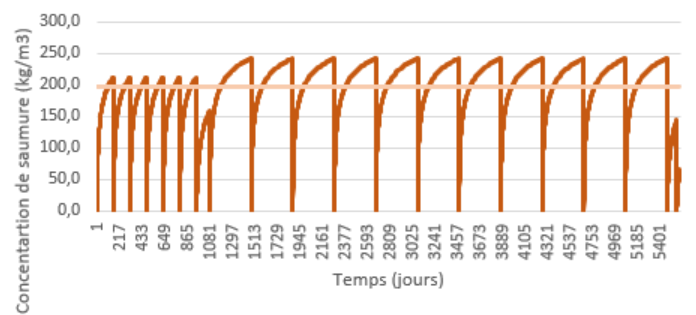
\includegraphics[width=\linewidth]{image/chap2/Graphe concentration C3 100.png}
    \caption{ }
  \end{subfigure}
  \begin{subfigure}[b]{0.43\linewidth}
    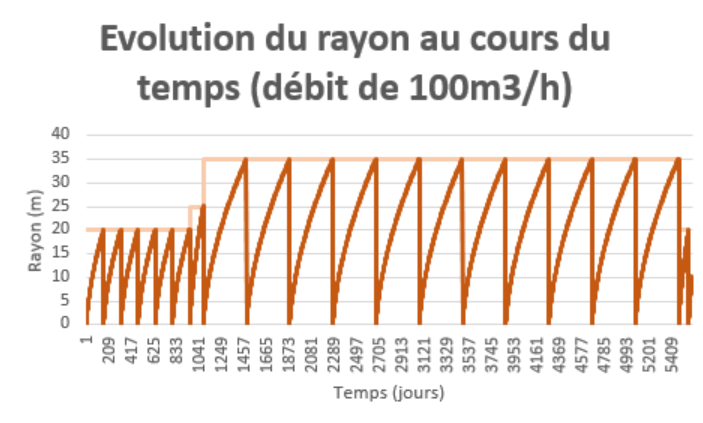
\includegraphics[width=\linewidth]{image/chap2/Graphe rayon C3 100.png}
    \caption{ }
  \end{subfigure}
  \caption{Evolution de la concentration de saumure (a) et du rayon (b) au cours du temps pour la configuration 3 }
\end{figure}

Nous remarquons que la durée de création de la cavité pour la configuration 3 est extrêmement longue (plus de 5500 jours, ce qui correspond à plus de 15 ans), nous avons donc essayé d’optimiser ce temps en doublant le débit (100 à 200 $m^3/h$), en sachant que cela allait diminuer la concentration de saumure. On obtient donc une durée plus raisonnable : 3500 jours, ce qui correspond à moins de 10 ans (voir graphes en annexes). En ce qui concerne la configuration 1, la création dure 470 jours, nous n’avons donc pas modifié le débit. 

En général la couche de sel n’est pas pure, il y a donc des impuretés dans la couche que nous appelons “insolubles”. Nous avons considéré un taux global homogène d’insolubles de 10\% dans la couche que l’on dissout, qui peut être sous la forme de couches épaisses qu’il est nécessaire de faire s’effondrer dans le puisard (partie de la cavité dédiée à recueillir les insolubles) ou bien de petits éléments épars dans la couche. 
Les graphiques montrant l'évolution du rayon et de la concentration de saumure pour la configuration 1 et la 3 optimisée sont en Annexe G, tout comme la méthode de gestion des insolubles.

\subsubsection{Création des cavités minées revêtues}

Dans cette partie, nous nous intéressons à la création des cavités minées pour le stockage souterrain d’hydrogène sous phase gazeuse. A la différence des cavités salines, les roches minées ne disposent pas d’une étanchéité naturelle et le coût des travaux est nettement plus important que le simple lessivage. Les techniques pour creuser les galeries et la cavité sont déjà bien connues, notamment celle dite des longs trous dont la méthode est détaillée en Annexe H pour la création de la cavité elle-même. Creuser les galeries est aussi bien maîtrisé par les ingénieurs.

Une cavité de stockage de gaz naturel en cavité minée revêtue a été réalisée dans un terrain granitique a Skallen en Suède avec un volume de $40000 m^3$. Il est intéressant de remarquer que la taille de ce type de stockage est beaucoup plus petite que les cavités salines. Nous nous sommes basés sur ce projet pour déterminer la technique de revêtement de la paroi.
Le revêtement est constitué de:

\begin{itemize}
\item Un béton projeté d’épaisseur maximale 0.7m mis en place au moment du creusement et permettant d’assurer une surface régulière (tolérance sur les hors-profils de ±0.3m).
\item Un système de drainage installé dans le béton projeté à proximité de l'interface avec la roche pour évacuer l'eau interstitielle.
\item Un revêtement de béton de génie civil armé de 0.7m d'épaisseur qui permet le transfert  uniforme de la pression du gaz au terrain, une bonne répartition des déformations du terrain dans le revêtement jusqu’à l’interface béton-acier. Le ferraillage permet aussi de disperser les fissures et de les partager en micro-fissures pour empêcher qu’elles puissent pénétrer dans le liner métallique.
\item Un liner métallique de 12 à 15 mm qui a pour objectif d'assurer une barrière imperméable (étanchéité).
\item Un liner bitumineux d'épaisseur 5 mm intercalé entre le béton et l’acier pour éviter la transmission des déformations du terrain à l’acier. Il autorise ainsi un mouvement relatif du liner par rapport au béton et permet que l’ensemble du revêtement résiste aux déformations mécaniques.
\end{itemize}

\begin{figure}[h]
  \centering
  \begin{subfigure}[b]{0.4\linewidth}
    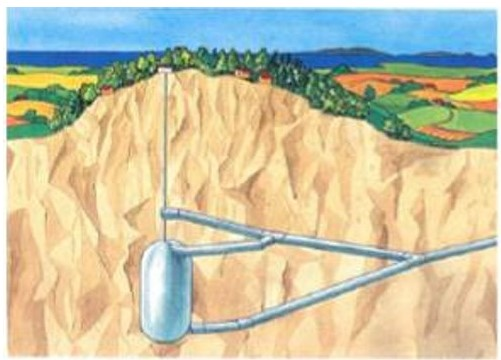
\includegraphics[width=\linewidth]{image/chap2/cav_skallen.jpg}
    \caption{ }
  \end{subfigure}
  \begin{subfigure}[b]{0.43\linewidth}
    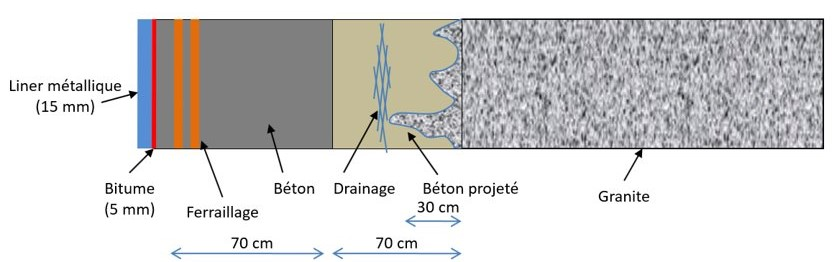
\includegraphics[width=\linewidth]{image/chap2/crea_cav_min.jpg}
    \caption{ }
  \end{subfigure}
  \caption{Cavité minée revêtue de Skallen (a) et revêtement associé (b)}
\end{figure}

Selon les scénarios, il est nécessaire de multiplier les cavités car celles-ci sont limitées en taille. Enfin, suite aux contraintes exercées sur les parois, on ne peut pas disposer aléatoirement les cavités dans les scénarios où il y a plusieurs cavités. Le détail des calculs est donné en annexe. Il faut retenir que pour conserver une marge de sécurité suffisante, chaque cavité doit être éloignée d’une distance au moins égale au double de son diamètre. Le détail des calculs est exposé en Annexe H.












\section{Chapitre III : Production, conditionnement et transport}
La synthèse d'hydrogène n'est pas récente. Cependant, si l'hydrogène doit devenir un vecteur énergétique majeur dans une société décarbonée, cela impose de revoir toute la chaîne de procédés: de sa production jusqu'à sa consommation. A partir des configurations types détaillées en chapitre 1, nous dimensionnons ces procédés.
\subsection{Production d'hydrogène bas carbone}
Les réactions thermodynamiques qui amènent à la production d'hydrogène sont toutes défavorisées: il faut donc amener des sources exterieures d'énergie. Il existe de nombreuses façons de synthétiser de l'hydrogène mais seules des productions bas carbone de celui-ci sont détaillées dans cette étude.  Actuellement, l'hydrogène est  produit à 96\% à partir de ressources fossiles \cite{Surla2019}. Deux synthèses sont ici détaillées: le vaporeformage qui utilise du gaz naturel (la technique la plus commune) et l'électrolyse de l'eau. Il existe d'autres procédés, certains encore au stade de développement. On peut citer en exemple l'injection d'eau sous pression dans des terres à forte teneur en fer pour faire de l'oxyde de fer et de l'hydrogène.

\subsubsection{Technologie SMR et CCS}
La vaporeformage, ou \emph{Steam Methane Reforming} (SMR), est la technique de synthèse d'hydrogène la plus commune. Elle utilise du gaz naturel et est émettrice de gaz à effet de serre. Nous n'envisageons donc la production d'hydrogène par SMR que couplée  avec un procédé de capture de $CO_2$ (CCS). $48 \% $ de l'hydrogène est actuellement produit par SMR. Les autres procédés fossiles utilisent du naphta ou du charbon (resp. 30\% et 18\%) [5]. \\  
Les unités de grande taille de production d'hydrogène atteignent aujourd’hui une production de $220000 Nm^3/h$. C'est sans conteste le procédé le moins cher et le plus efficace.

\begin{center}
\begin{figure}[!h]
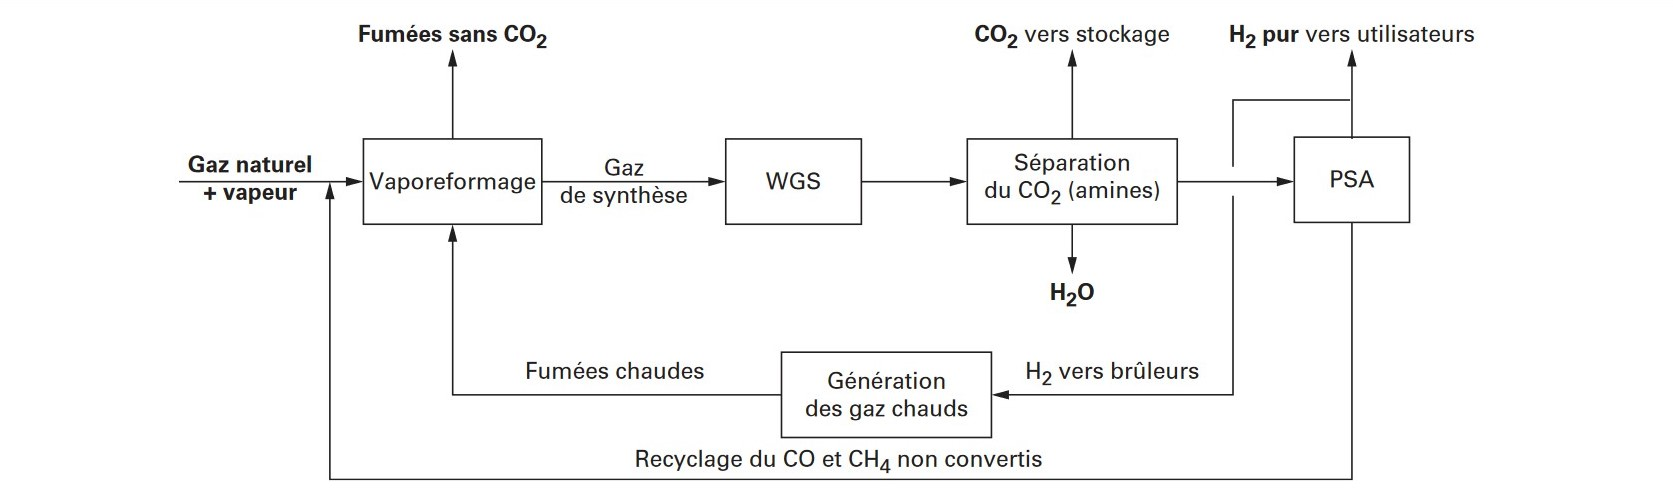
\includegraphics[width=0.95\linewidth]{image/chap3/Vapo_avec_sequestration.jpg}
\caption{Technique de vaporeformage avec séquestration de $C0_2$ \cite{Prod_gaz_synth}}
\end{figure}
\end{center}

Les étapes de production sont les suivantes:
\begin{enumerate}
\item Il faut dans un premier temps traiter les composants chlorés et souffrés qui endommagent les catalyseurs lors de la suite du processus. Le souffre est éliminé dans des réacteurs d’adsorption à l’oxyde de zinc \cite{Prod_gaz_synth}
 avec la réaction $$ H_2S + ZnO \rightarrow ZnS + H_20 $$ 

\item Le gaz naturel et les hydrocarbures légers sont ensuite transformés en gaz de synthèse par vaporeformage. La conversion du méthane est favorisée par une haute température, une basse pression et un large excès de vapeur d’eau. Des bruleurs fonctionnant àl'aide d'$H_2$ assurent la température. La réaction SMR : $$ CH_4 + H_2O \rightarrow CO + 3H_2 , \Delta H_{760\celsius}=226kJ/mol$$

\item Ensuite on effectue en \emph{Water Gas Schift} (WGS) pour convertir $CO$ en $CO_2$. On souhaite augmenter la teneur en $H_2$ dans le gaz de synthèse avant la purification finale. La conversion du CO est favorisée à basse température et en large excès de vapeur d’eau \cite{Prod_gaz_synth}. La réaction WGS : $$ CO + H_2O \rightarrow CO_2 + H_2 , \Delta H_{760\celsius} =-34,3kJ/mol$$

\item Le $CO_2$ produit est ensuite récupéré par absorption par des amines dans une solution aqueuse. $C0_2$ est séparé de $H_2$. Il existe d'autres technologies en développement comme la récupération par cryogénie, développée par \emph{Air Liquide}.

\item L'hydrogène est ensuite purifié dans des unités PSA. Le PSA est un procédé de séparation basé sur l’affinité des différents composés d’un fluide pour un adsorbant solide à la surface duquel certains composés s’adsorbent. L'hydrogène ressort enfin pur. 

\end{enumerate}

On peut maintenant caractériser la technique SMR par ordres de grandeur.
\begin{itemize}
\item Charge : Pour produire $1kg$ de $H_2$ il faut environ $3,7kg$ de gaz naturel \cite{Prod_gaz_synth}.
\item La taille d'une unité SMR est comprise entre $10000$ et $200000 Nm^3/h$  \cite{Prod_gaz_synth}
\item Séquestration du carbone : les unités de capture actuelles du $CO_2$ nécessitent en moyenne entre $750$ et $1100kWh/ton CO_2$. On pense atteindre $300 kWh/t CO_2$ avec des nouvelles technologies \cite{Surla2019}.
\item Le $CO_2$ est capturé à hauteur de 80 à 95\%. 1 kg d'$H_2$ produit génère donc $ 5,5 kg \times 0.10 = 550 g$ de $CO_2$ \cite{Surla2019}.
\item Le prix d'un SMR type d'une unité de production d’hydrogène à partir du gaz naturel d’une capacité de $100000 Nm^3/h$ avec purification de l’hydrogène par PSA (pureté 99,9 \% en volume, taux de récupération d’environ 90 \%) représente un investissement d’environ 120 M€.
\end{itemize}


\subsubsection{L'électrolyse de l'eau}

Contrairement au vaporeformage, l’électrolyse utilise principalement de l’énergie électrique pour produire de l’hydrogène gazeux. Cela correspond à la réaction d'oxydo-réduction : 
$$H_2O_{liq} \rightarrow H_2 + \frac{1}{2} O_2 , \Delta H^0 (298 K) = 286 kJ/mol $$
Le signe positif de l’enthalpie signifie que la réaction est endothermique.
Il y a plusieurs façons d’exploiter cette réaction à travers des demi-réactions différentes. Nous nous sommes intéressés à trois technologies:\\

\begin{enumerate}
\item L’électrolyse à oxyde solide : Les électrolyseurs utilisant cette méthode sont composés d’une anode en LSM (Manganite de lanthane dopé au strontium), et une cathode en nickel. Les demi-réactions mis en jeu étant pour l’anode :  $2 O_2^- \rightarrow O_2 + 4 e^- $, et pour la cathode : $H_2O + 2 e^- \rightarrow H_2 + O_2^- $ . Cet électrolyseur nécessite une eau à haute température, un électrolyte pour faire migrer les ions et a une faible densité de courant. 

\item L’électrolyse alcaline : l’anode de ces électrolyseurs est à base de titane ou de nickel, et la cathode est en acier. Les réactions ayant lieu étant alors pour l’anode :  $2 OH^- \rightarrow H_2O + 1/2 O_2 + 2e^- $, et pour la cathode : $2 H_2O + 2 e^- \rightarrow H_2 +2 HO^- $ . Cet électrolyseur fait intervenir une migration lente des ions OH- à travers une membrane dans un électrolyte, et une faible densité de courant.

\item L’électrolyse PEM (Proton Exchange Membrane) : l’anode de ces électrolyseurs est faite en oxyde d'iridium (IrO2) ou de ruthénium (RuO2), et la cathode est en platine. Le fer et le cobalt catalysent la réaction eux aussi mais sont instables dans les conditions de la réaction, d’où l’utilisation du platine. Les réactions aux électrodes sont pour l’anode (1) et la cathode (2):  
$$2H_2O \rightarrow O_2 + 4H^+ + 4e^- \  (1) \ \ \ , \ \ \ 4H^+ + 4e^-  \rightarrow 2H_2  \ (2)$$

Dotés d’un temps de réponse de l’ordre de la milliseconde et pouvant supporter de grandes intensités, nous allons choisir ces électrolyseurs. Il faut néanmoins prendre en compte le fait que des métaux rares sont utilisés dans sa fabrication, notamment de l'iridium pour catalyser la réaction, ce qui est un réel frein au développement industriel de l'électrolyse PEM.

\end{enumerate}

\begin{table}[h]
\centering
\begin{tabular}{|l|l|l|l|l|}
\hline
Electrolyseurs & Oxyde solide & Alcalins & PEM \\
\hline
Densité de courant maximal & 2 A/cm2 &0,5A/cm2 & 3A/cm2 \\
\hline
Puissance d’un stack & 150KW& 2,5MW - 5MW&3MW \\
\hline
Température de fonctionnement &650-1000 °C&70-90 °C&50-70 °C\\
\hline
Pression de fonctionnement&1 bar& 0,3 - 30 Bar & Jusqu'à 35bar \\
\hline
\end{tabular}
\caption{Caractéristiques des différents électrolyseurs $[VII]$}
\end{table}

\begin{figure}[h]
  \centering
  \begin{subfigure}[b]{0.3\linewidth}
    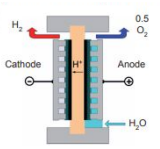
\includegraphics[width=\linewidth]{image/chap3/Figure 3.2.b-2.png}
    \caption{Pile d'un électrolyseur PEM.}
  \end{subfigure}
  \begin{subfigure}[b]{0.4\linewidth}
    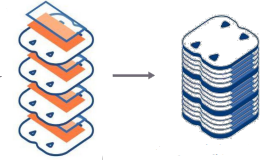
\includegraphics[width=\linewidth]{image/chap3/Figure 3.2.b-3.png}
    \caption{Formation d’un stack à partir de plusieurs unités.}
  \end{subfigure}
  \caption{Une pile PEM}
\end{figure}

On peut maintenant caractériser la pile PEM par ordre de grandeur:
\begin{itemize}
\item Les unités sont regroupées pour former des stacks (Figure 20(b))
\item La réaction d’électrolyse ayant une enthalpie de $\Delta H = 280 KJ/mol$
\item La tension de fonctionnement est alors de $U= \Delta H^0 /n\times \mathfrak{F} =1,4 V$ avec $n$ le nombre d’électrons échangés et $\mathfrak{F}$ la constante de Faraday. La tension varie en pratique entre $1,23V$ et $1.48V$. 
\item Cette enthalpie nous permet de déduire qu’il faut théoriquement $38KWh$ d'énergie pour 1kg de $H_2$.
\item Avec un rendement d’électrolyseurs de 70\% cette énergie peut monter à 55kWh par kilogramme de $H_2$
\end{itemize}

\subsection{Conditionnement de l'hydrogène}

L’hydrogène, après avoir été produit par électrolyse ou SMR, doit être conditionné en amont et en aval du stockage en cavité. Pour dimensionner ce conditionnement, il convient de réfléchir sur l’état de stockage ou de transport de l’hydrogène, à savoir gazeux ou liquide.

Pour appréhender cette partie, il est bon de retenir que le LH2 est plus dense énergétiquement et permet de baisser le coût global d'une chaîne de procédés si le transport est effectué sur des grandes distances ou en grandes quantités. Dans le cas contraire, on préfèrera le GH2. En effet, pour deux camions de poids identiques de $36t$, le premier a une capacité de $4500 kg LH_2$ tandis que pour le second, de seulement $300 kg GH_2$ [V]. Notons aussi que le stockage ou transport sous forme liquide garantit une meilleure sécurité des installations.

\subsubsection{Compression}

L'hydrogène sort de l'électrolyseur à 3 MPa et à 60°C, et de la station SMR à 2 MPa et à 27 °C. La pression d'injection de l'hydrogène en cavité saline (14 à 15 MPa) et minées revêtues (18 MPa) étant supérieure à celle de sortie de l'électrolyseur, il faut donc comprimer le gaz. En sortie de la cavité, il est parfois nécessaire de recomprimer le gaz (qui s’est détendu en sortant de la cavité), mais nous avons décidé de ne pas étudier cette étape dans notre étude. 

D'un point de vue technique, le taux de compression ne peut techniquement pas dépasser 3, c'est-à-dire que la pression de sortie doit être inférieure à trois fois la pression d'entrée. De plus, la température dans le compresseur ne doit pas excéder 150°C afin de ne pas l'endommager [VI]. Par conséquent, il est nécessaire de refroidir l'hydrogène en sortie du compresseur avec des échangeurs et d'utiliser plusieurs étages de compression. 

Pour ce faire, nous avons, à l’aide du diagramme des frigoristes de l’hydrogène, réalisé une étude thermodynamique simple pour dessiner les différents étages de compression, puis les avons modélisés à l’aide du logiciel \emph{ASPEN PLUS}, couramment utilisé dans l'industrie notamment dans le domaine de la thermodynamique des procédés. L'annexe I détaille l'outil \textit{Aspen Plus} et ses crédits.

En ce qui concerne le choix des compresseurs, nous avions le choix entre des compresseurs volumétriques et dynamiques. Après des recherches bibliographiques, le choix du compresseur volumétrique nous a paru le plus pertinent au vu des propriétés volumiques de l’hydrogène (densité)[VII]. Nous l’avons modélisé sur \emph{ASPEN PLUS} comme un compresseur idéal isotherme. Pour les échangeurs, le liquide réfrigérant utilisé est de l’eau. Un exemple de schéma du procédé de compression entre la phase de production et de stockage, pour la configuration 1, est donné par la figure 20.\\

\begin{figure}[h!]
 \centering
 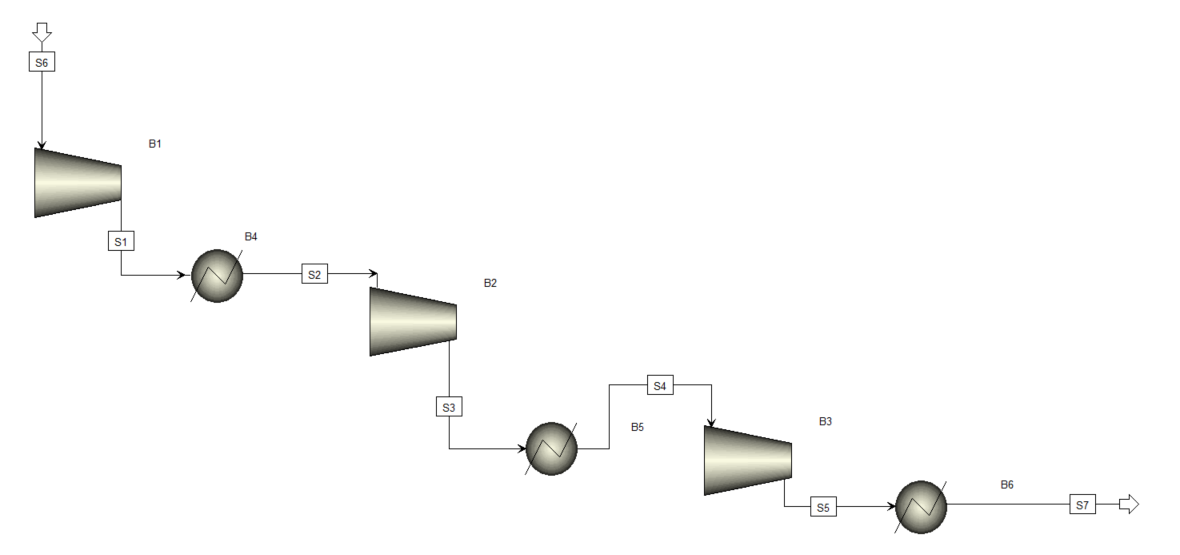
\includegraphics[width=.8\linewidth]{image/chap3/etage_compression.PNG}
 \caption{Procédé de compression modélisé avec \textit{ASPEN PLUS} pour la configuration 1}
\end{figure}



\subsubsection{Liquéfaction}


\begin{multicols}{2}
On cherche à liquéfier l'hydrogène pour augmenter sa densité énergétique. Liquéfier l'hydrogène pour le transporter ou le stocker est un défi technique de taille : l'hydrogène est liquide à une température inférieure à 20K à pression athmosphérique (cf. figre 21). Il s'agit donc de dimensionner et caractériser un ensemble de cycles thermodynamiques pour refroidir l'hydrogène. 

De plus, la liquéfaction de l'hydrogène présente un défi de nature quantique : la conversion orthohydrogène-parahydrogène. On parle de deux isomères de l'hydrogène. Pour l'orthohydrogène le proton de chaque molécule d'hydrogène possède des spins parallèles, pour le parahydrogène le proton de chaque molécule d'hydrogène possède des spins antiparallèles.


\begin{center}
  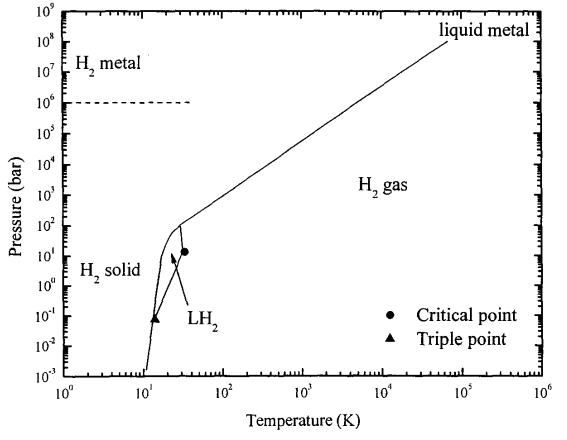
\includegraphics[width=\linewidth]{image/chap3/diagramme de phase H2.png}
  \captionof{figure}{Diagramme de phases de l'hydrogène}
\end{center}

\end{multicols}

\begin{figure}[!h]
  \centering
  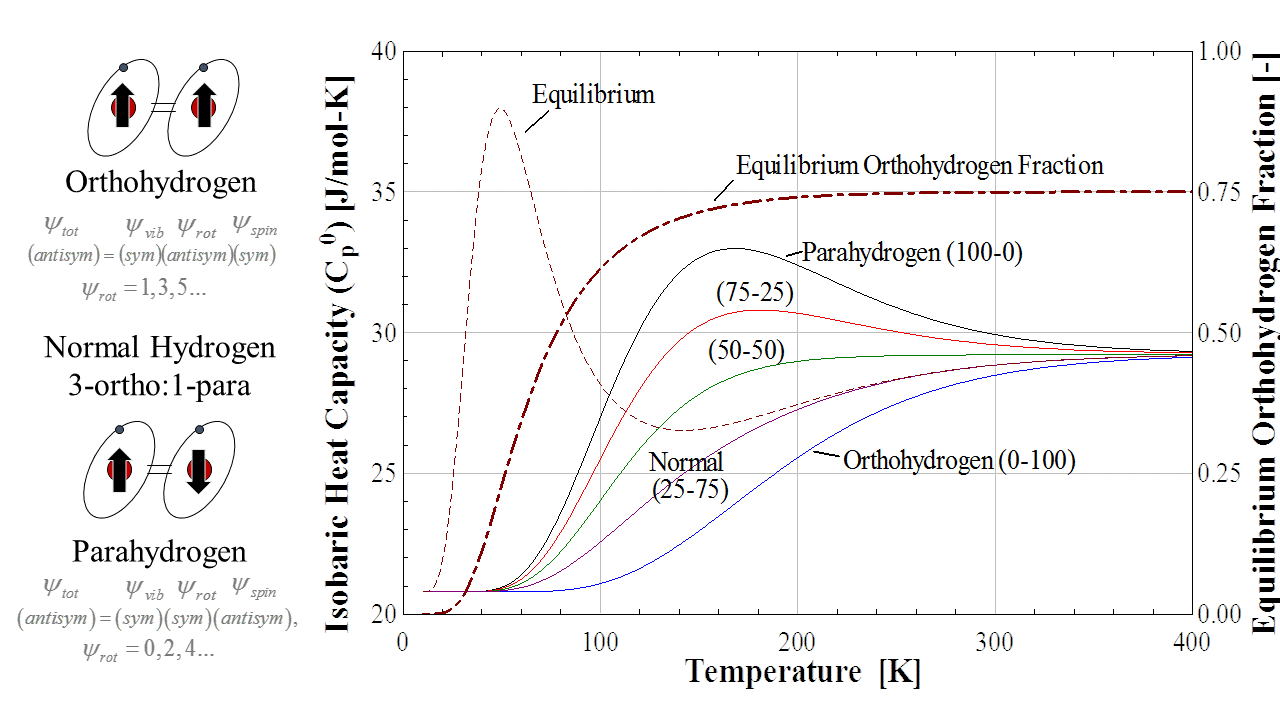
\includegraphics[width=0.6\linewidth]{image/chap3/Ortho-para.png}
 \caption{Proportion ortho-para en fonction de la température et énergie de conversion \cite{orthopara}.}
\end{figure}


A 300 K, il y a 25\% de parahydrogène et 75\% d'orthohydrogène. A 20K, il y a 100\% d'orthohydrogène. On observe donc une conversion orthohydrogène à parahydrogène. Or, cette réaction est fortement exothermique (cf. figure 22): 
 $$ \Delta h _{conv} = 500kJ/kg$$
En cherchant à refroidir à de l'hydrogène on le réchauffe. L'équilibre s'atteint en quelques jours : c'est une réaction assez lente.

\begin{figure}[h]
  \centering
  \begin{subfigure}[b]{0.4\linewidth}
    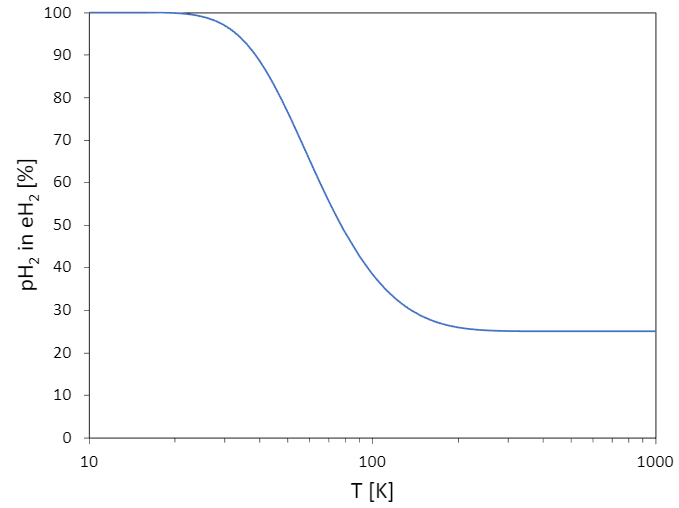
\includegraphics[width=\linewidth]{image/chap3/proportion_o-p.png}
    \caption{ }
  \end{subfigure}
  \hspace{0.1cm}
  \begin{subfigure}[b]{0.4\linewidth}
    \includegraphics[width=\linewidth]{image/chap3/énergie-conversion.png}
    \caption{ }
  \end{subfigure}
  \caption{Proportion ortho-para (a) et énergie nécessaire à la conversion ortho-para en fonction de la température (b).}
\end{figure}

La conversion ortho-para est aussi une des causes de \emph{boil-off} dans les stockages : l'hydrogène liquide s'évapore et cela cause des surpressions dans les cavités. Il faut donc impérativement envisager la conversion ortho-para lors de la liquéfaction. Il existe des catalyseurs de la réaction de conversion et ceux-ci sont positionnés dans la chaîne de liquéfaction. 

Plusieurs cycles thermodynamiques sont décrits dans la littératures pour liquéfier l'hydrogène. Nous avons fait le choix de synthétiser ceux-ci et de présenter un cycle simplifié. Ce cycle a le mérite d'exposer les ordres de grandeurs. Nous avons utilisé sa représentation sous \emph{ASPEN PLUS} pour en faire l'évaluation économique.

\begin{figure}[h!]
\centering
\includegraphics[width=0.9\linewidth]{image/chap3/liquéfaction.png}
\caption{Représentation simplifiée avec \textit{ASPEN PLUS} de la liquéfaction}
\end{figure}

Nous détaillons ici les différentes étapes de la liquéfaction. On suppose que l'hydrogène gazeux arrive sous pression de 2 MPa et à 27°C (sortie de vaporeformage).
\begin{enumerate}
\item L'hydrogène est d'abord comprimé jusqu'à une pression de 3 MPa. On négligera les pertes de charges par la suite.
\item L'hydrogène est amené à 20°C avec des échangeurs à eau liquide.
\item L'hydrogène est refroidi dans un bain d'azote liquide. Il ressort à 80K.
\item L'hydrogène est refroidi par la détente d'hélium jusqu'à 30K.
\item On symbolise la conversion ortho-para par un échangeur de chaleur qui réchauffe le fluide super-critique. Il ressort à 30 bars et 55K.
\item On effectue un deuxième refroidissement par la détente d'hélium gazeux jusqu'à 20K.
\item On effectue une détente Joule-Thomson (enthalpique) jusqu'à pression atmosphérique. De super-critique, le fluide d'hydrogène devient diphasé avec une proportion de 70\% de $LH_2$.
\item On sépare les deux phases dans un séparateur.
\end{enumerate}


Une fois liquide, l'hydrogène a alors une masse volumique de $70,973 kg/m^3$ à pression atmosphérique et à $20,28K$ \cite{Surla2019}. Cela donne un pouvoir calorifique de $9,93 MJ/L$ soit environ 4 fois moins que l'essence mais 780 fois plus grand que l'hydrogène gazeux à pression atmosphérique. On peut envisager toutes sortes d'optimisation des procédés, comme par exemple la réutilisation de l'hydrogène gazeux très froid pour refroidir l'hydrogène plus chaud. L'annexe I décrit le principe de modélisation du procédé de liquéfaction sous \textit{Aspen Plus} et les équations fonctionnelles utilisées dans le logiciel.
L'annexe J détaille le procédé de liquéfaction.

\subsection{Transport d'hydrogène}
Le transport de l'hydrogène pose des problèmes techniques nouveaux de part sa nature thermodynamique. Il peut être envisagé sous deux conditionnements différents. Premièrement sous forme gazeux par pipeline ou camion, mais aussi sous forme liquide par camion ou bateau.

\subsubsection{Transport de $GH_2$}

Transporter du gaz pose un problème technique: les pertes de charges dans les conduites. On désigne par charge la quantitée $\Pi = p+\rho g z + \frac{1}{2}\rho v^2$, avec $p$ la pression, $ \rho$ la masse volumique et $v$ la viteese du fluide. Cette quantitée diminue au cours de l'écoulement, à travers les différents éléments du réseau. Les pertes de paroi sont dûes à la viscosité du fluide et les pertes singulières au décollement du fluide des interfaces, ce qui redistribue les cartes de vitesse.

Dans le cas d'un fluide incompressible dans une conduite horizontale de rugosité relative $\frac{\epsilon}{D}$, on a une perte de charge $$ \Delta \Pi = \frac{1}{2} \rho v^2 \lambda ( Re, \frac{\epsilon}{D}) $$ et on lit $\lambda ( Re, \frac{\epsilon}{D}) $ sur les diagrammes de \emph{MOODY} sachant que l'$H_2$ est compressible.

Lorsqu'une canalisation est parcourue par un fluide compressible, la masse volumique $\rho$ décroit dans le sens du courant à cause de la chute de pression. Par conservation du débit, la vitesse $V$ augmente. \\ Puisque chaque tronçon $dx$ n'est plus comparable car dans chacun d'eux la pression est différente, on décrit la perte de charge sur chaque tronçon et on intègre. 
On a en régime turbulent: 
$$
 	dp + \rho V dV= -\frac{\lambda}{2}\rho v^2 \frac{dx}{D} \ \ , \ \
 	\rho V =cte  \ \ , \ \
 	T_{ext}=cte  \ \ , \ \
 $$
 
Et on trouve alors:
$$ p_1^2 - p_2^2 =2 p_1 \rho_1 v_1^2 (\frac{\lambda L}{2 D} + ln\frac{p_2}{p_1}) $$

\begin{multicols}{2}

Transporter du gaz par pipeline est donc couteux en énergie à cause des pertes de charges. Tous les 100km on perd 1,2\% de l'énergie transportée. De plus, l'hydrogène est une molécule très petite. On assiste donc à des phénomènes de fragilisation des matériaux.

Pour des courtes ou moyennes distances, le transport par camion est plus adapté. En effet, la construction de pipeline est onéreuse (un million d’euros par kilomètre en ordre de grandeur) et le transport d’hydrogène gazeux par un pipeline soulève de nombreux problèmes techniques. Ainsi on peut transporter l’hydrogène gazeux comprimé dans des bouteilles. Il en existe deux types, le premier est une bouteille entièrement en acier, et l’autre alternative, plébiscitée par Airliquide, est une bouteille composée de plusieurs matériaux ( cf. figure 25). Ces bouteilles sont composées premièrement d’une structure en fibre de carbone garantissant la résistance aux efforts mécaniques. Cette structure recouvre une épaisse couche d’acier sur laquelle repose un liner en polymère qui garantit l’étanchéité de la bouteille. On peut alors comprimer l’hydrogène à 500 bar et stocker de 5 à 10 kg par bouteille \cite{MAHYTEC}. Un camion peut ainsi transporter 300 kg d’hydrogène [V].

\begin{center}
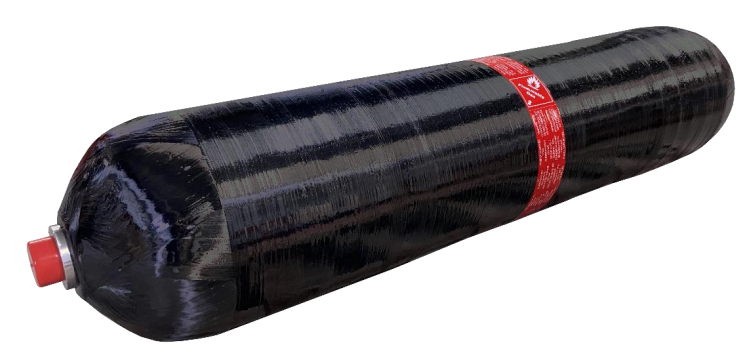
\includegraphics[width=.8\linewidth]{image/chap3/Figure 3.i-1.png}
\captionof{figure}{Bouteille en matériaux composites}
\end{center}

\end{multicols}

\subsubsection{Transport de $LH_2$}

\begin{multicols}{2}

Tout l’intérêt de l’hydrogène liquide réside dans son transport en comparaison avec sa forme gazeuse. En effet, l’hydrogène liquide est plus dense énergétiquement que l’hydrogène gazeux. Selon Air Liquide, pour un poids de camion identique (36 tonnes), on peut transporter jusqu’à 4500 kg d’hydrogène sous conditionnement liquide contre seulement 300 kg sous conditionnement gazeux, soit 15 fois plus [V].

Ainsi on pourrait envisager le transport de l’hydrogène liquide par camion pour les courtes à moyennes distances, et par bateau pour les longues distances. Concernant le transport d’hydrogène liquide par camion, il s’effectue dans des citernes pouvant transporter de grandes quantités d’hydrogène liquide [V]. C’est le moyen de transport pour lequel nous avons opté pour les configurations 5, 6 et 7. Concernant la configuration 6, il s’agit d’un stockage en cavité minée revêtue d’une capacité de 230 tonnes d’hydrogène liquide se situant à 240 km du lieu d’utilisation. Il faudrait alors 50 camions par jour pour transporter l’hydrogène sous conditionnement liquide. Pour la configuration 7, il s’agit aussi d’une cavité minée revêtue, mais d’une capacité plus faible (143 tonnes) et relativement proche du lieu d’utilisation (12 km). Ainsi, il faudrait en théorie 30 camions par jour, cependant étant donné la faible distance séparant les lieux de stockage et d’utilisation, on pourrait réduire le nombre de camions en leur faisant effectuer plusieurs fois le trajet.\\

Concernant le transport par bateau, un projet pilote est actuellement en cours (Figure 26). Il s’agit du « Suiso Frontier », destiné à relier l’Australie au Japon, et dont la capacité est de 1250 m3 (soit près de 90 tonnes d’hydrogène liquide \cite{The_Suiso_Frontier}. Ce moyen de transport n’est pas nécessairement intéressant pour nos scénarios, étant donné que tout est localisé en France. Cependant, comme pour le projet pilote, il devient très intéressant lorsque l’on veut transporter de l’hydrogène d’un continent à un autre. Ainsi, cela pourrait être particulièrement pertinent si l’on envisage que l’hydrogène tienne un rôle important dans la transition énergétique.

\begin{center}
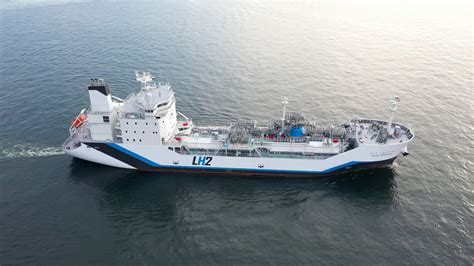
\includegraphics[width=.9\linewidth]{image/chap3/Figure 3.ii-3.jpg}
\captionof{figure}{Projet pilote Suiso Frontier}
\end{center}

\end{multicols}

\subsection{Applications aux configurations retenues}


\begin{figure}[!h]
  \centering
  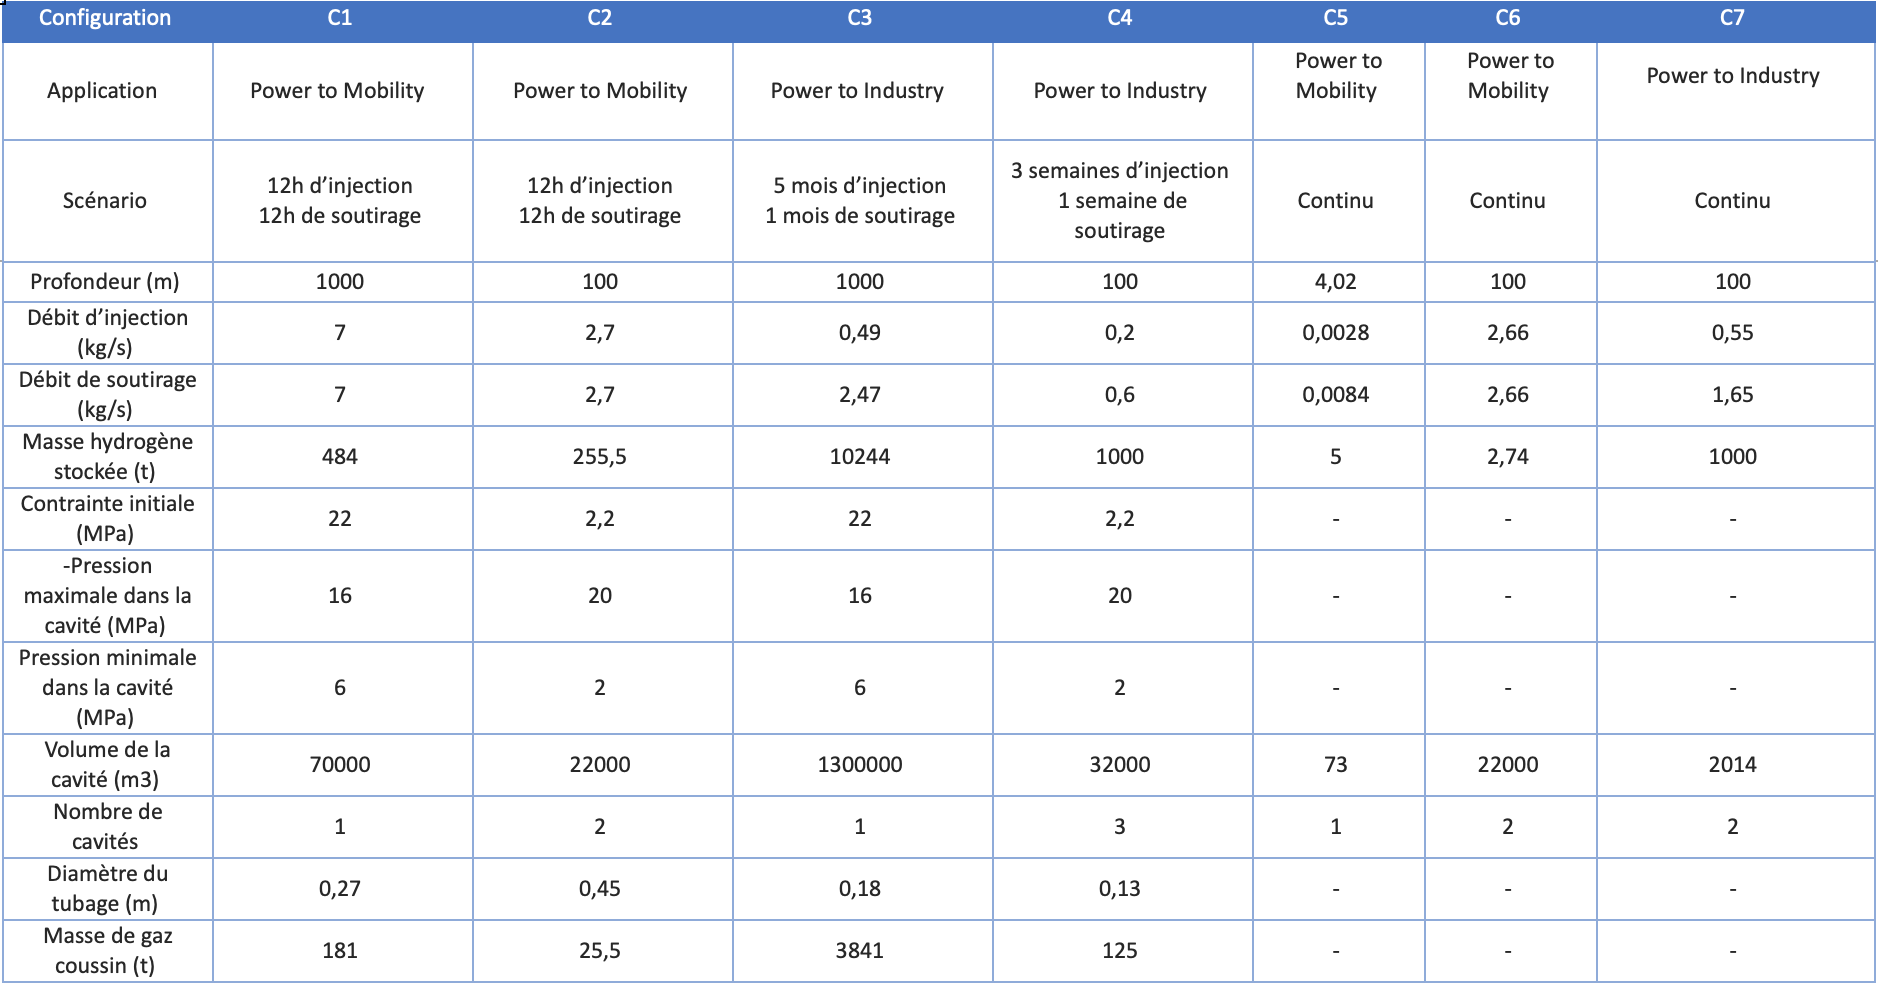
\includegraphics[width=0.9\linewidth]{image/chap3/Tableau 1 chap 2.4.png}
  \caption{Récapitulatif des paramètres nécessaires au dimensionnement des stockages des différentes configurations}
  \end{figure}


\begin{figure}[!h]
\centering
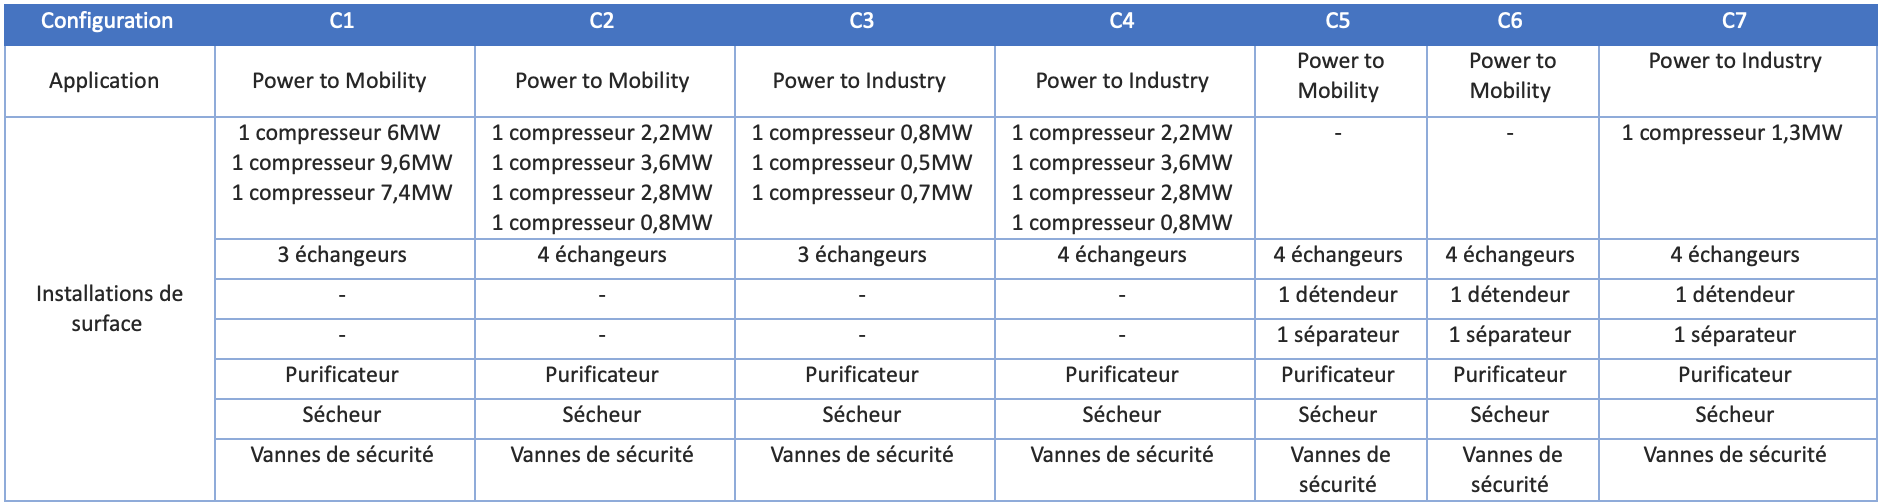
\includegraphics[width=0.9\linewidth]{image/chap3/Tableau 2 chap 2.4.png}
\caption{Récapitulatif des installations de surface pour les différentes configurations}
\end{figure}

Les simulations numériques du comportement thermomécanique du stockage des configurations nous ont permis de valider ou d'ajuster certains paramètres en jeu. Nous avons extrait de ces simulations 7 applications industrielles ou de mobilité qui ont été étudiées dans le détail.

La figure 27 regroupe les paramètres des configurations de stockage retenues pour les 7 applications industrielles ou de mobilité, tandis que la figure 28 résume les installations de surface qui leur sont associées et les puissances électriques mobilisées.


Chaque configuration étudiée peut être synthétisée par un \textit{flowsheet}. Un \textit{flowsheet} permet d'indiquer les différents flux physiques qui rentrent ou sortent dans chacune des étapes d'un procédé, d'où son nom. C'est un outil très pratique de visualisation d'un procédé qui permet d'identifier aisément les différentes dépendances. La figure 29 en donne une illustration.

\begin{figure}[!h]
\centering
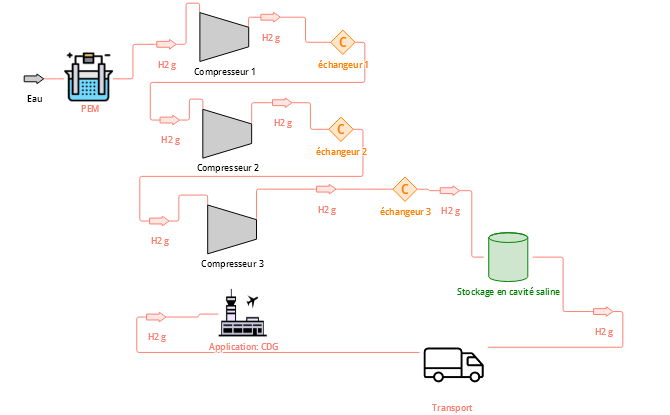
\includegraphics[width=0.7\linewidth]{image/chap3/figure2_chap2.4.png}
\caption{ \textit{Flowsheet} des installations de surface de la configuration 1.}
\end{figure}






\section{Chapitre IV : Impacts environnementaux et sociétaux}
\subsection{Réglementation}

Afin de stocker de l’hydrogène en souterrain, il est nécessaire d’effectuer plusieurs procédures administratives. L’installation de la cavité est réglementée par le code minier (articles 211-1 et suivants).
Tout d’abord, la possession d’un titre minier (Livre I – Titres II à IV + décret 2006-648) est nécessaire pour pouvoir construire la cavité souterraine. Si le stockage est supérieur à 100 kg d’hydrogène, ce qui correspond au seuil des Installations Classées pour la Protection de l’Environnement (ICPE), on est soumis au code minier mais aussi au code environnemental. Dans ce cas, les travaux suivent la directive SEVESO, directive européenne qui encadre les sites industriels à risque majeur. 
L’installation peut ainsi être classée selon un seuil SEVESO bas ou un seuil SEVESO haut (ce qui dépend de la quantité stockée). Dans le cas contraire, on est soumis aux titres VI du livre II du code minier, le décret n°2006-649 du 2 juin 2006 relatif aux travaux miniers, aux travaux de stockage souterrain et à la police des mines et des stockages souterrains, le décret n°2016-1303 du 4 octobre 20164 relatif aux travaux de recherches par forage et d’exploitation par puits de substances minières (dit décret « forage »), et l’arrêté ministériel du 14 octobre 2016. Si la cavité existe déjà, il faut déclarer qu’on modifie un ICPE déjà existant au Préfet, s’il juge que les modifications sont notables, une demande doit être déposée selon le code de l’environnement. Celle-ci doit contenir une étude de dangers (L181-25 + D181-15-2-III) et une étude d’impact (L122-3 + R122-4 et 5) ou d’incidence environnementale (L181-8 et R181-14).


\subsection{Sécurité et risques environnementaux}

Pour comprendre les risques liés à l'utilisation de l'hydrogène, il faut tout d'abord étudier ses spécificités :
\begin{itemize}
\item Facilité à fuir : sa molécule est de petite taille et il possède une très faible viscosité.
\item Très faible énergie d'inflammation : de l'ordre de $17 \mu J/mole$ soit plus de 15 fois inférieure à celle du gaz naturel ($290 \mu J/mole$). Le risque d'inflammation est donc très grand
\item Flamme très peu éclairante : en effet le rayonnement de l'hydrogène chauffé se situe essentiellement dans le domaine ultra-violet. Cela constitue un danger supplémentaire pour les équipes d'intervention lors d'incendies.
\item Risque de détonation : en cas d'accumulation de l'hydrogène, d'énergie d'inflammation élevée ou de présence d'obstacles qui accélèrent la flamme, il peut y avoir détonation. Elle se caractérise par un front de flamme se déplaçant à vitesse supersonique accompagné d'ondes de choc.
\end{itemize}

L'opération de stockage (ici en cavité saline) présente aussi des risques tels que la rupture du massif de sel, la perte excessive de volume de la cavité ou la perte de l'étanchéité du sel. Pour l'hydrogène liquide, le boil-off reste le principal facteur de fuite. \cite{ADEME_2022}

Afin de prévenir les risques liés à l'hydrogène, il faut :
\begin{itemize}
\item Prévoir des détecteurs d'hydrogène près des points de fuite et d'accumulation potentiels.
\item Placer les sytèmes hydrogènes à l'extérieur des locaux.
\item Prévoir une ventilation permanente.
\item Limiter les raccords vissés et les montages et démontages fréquents.
\item Prévoir un dispositif de coupure automatique en cas de fuite.
\item Bien dimensionner le volume d'hydrogène stocké.
\end{itemize}

L'hydrogène est un gaz à effet de serre indirect, en effet, sur une période de 100 ans, il possède un potentiel de réchauffement global, noté PRG, de 11 en moyenne. Le PRG correspond au pouvoir réchauffant d'un gaz rapporté à celui du $CO_2$. En comparaison, celui du méthane est de 25. Ainsi, les fuites d'hydrogène accélèrent le réchauffement climatique.

De plus, lors du stockage, "une fuite dans des aquifères sous-jacents ou de couches superficielles est susceptible d'avoir des impacts environnementaux (contamination des aquifères d'eaux potables, d'éventuels ouvrages souterrains..)" selon ANCRE $[3]$.

L'hydrogène stocké peut aussi constituer une source d'énergie pour de nombreux microorganismes qui le consomment. Le nombre des microorganismes peut augmenter ce qui présente un risque de colmatage de la roche aquifère, et donc une diminution de la porosité. Une telle activité microbienne dans les aquifères modifie durablement les conditions physico-chimiques de l'eau.\\



\subsection{Acceptabilité}
L’étude de l’acceptabilité sociale est une phase cruciale de notre projet, il est donc nécessaire d’observer le lien entre les acteurs et les porteurs de sujet mais aussi les besoins de la population pour savoir si le stockage et l’utilisation de dihydrogène dans la société seront communément acceptés. L’ensemble des lois et des réglementations est régi par l’opinion publique, il est donc important d’avoir connaissance de cette opinion, afin de conserver une longueur d’avance dans la mise en place de notre projet.

De nombreuses études sociologiques ont déjà été menées notamment en Normandie avec l’étude VERTIGO en avril 2021. En effet, cette région a décidé de développer son réseau de bus circulant au dihydrogène. Il en ressort que malgré la méconnaissance du sujet par la plupart des usagers, ceux-ci y restent favorables car cette technologie est présentée comme écologique. Peu d’individus dénoncent les dangers liés au stockage d’hydrogène dans les bus. En revanche, la principale source d’inquiétude dans ce milieu plus rural où la mobilité tient une place essentielle dans la vie professionnelle est l’éventuel changement d’habitudes qu’amènerait cette transition à l’hydrogène.
Une autre étude sur l’acceptabilité du stockage souterrain se rapprochant plus explicitement de la nôtre, menée par l’université de Lorraine pour le projet ROSTOCK-H en octobre 2020, soulève les mêmes inquiétudes de la part de la population.

Nous avons donc mené notre propre enquête dont le détail a été développé en Annexe L. Sur 136 réponses, voici ce qu'il en ressort. La population étudiée avait en majorité (70.6\%) déjà quelques notions scientifiques du fait de leurs études ou leur travail et une partie affirme bien connaître le sujet (46.3\%). Les motivations restent portées par une conscience écologique mais les avis restent partagés sur la mise en place d’un tel projet et l’engouement ne semble pas aussi important que celui présenté par les médias. Seule une moitié (55.6\%) des individus interrogés annonce être prête à avoir des stockages souterrains à proximité de leur logement. Le dihydrogène est majoritairement retenu comme une solution dans le mix énergétique mais ne sera certainement pas le vecteur d’énergie dominant à l’avenir.


\subsection{Sites potentiels de stockage}
Nous nous intéressons ici au choix des sites de stockage en France, à la fois pour les cavités minées et salines, pour le stockage gazeux et liquide et pour les utilisations pour la mobilité et l'industrie. 
\subsubsection{Critères de choix}
Le choix des sites potentiels pour le stockage de l’hydrogène souterrain est dépendant de plusieurs critères : 
\begin{itemize}
\item critères géologiques : dans le cadre de la France métropolitaine, on dispose d’une géologie variée, comme on peut le voir sur la carte géologique fournie en annexe M. La profondeur, l’épaisseur et la pureté de la roche souhaitée entrent en jeu.
\item critères géographiques : la zone choisie nécessite une liaison au réseau électrique haute tension et un acheminement d’hydrogène. Dans le cas des cavités salines, il est également nécessaire de prendre en compte les possibilités d’acheminement de l’eau lors du creusement des cavités.
\item critères économiques : les perspectives économiques liées au marché et aux besoins hydrogène doivent être prises en compte. On s’intéresse notamment aux besoins et à la présence d’infrastructures de production d’énergies renouvelables à proximité, dans la perspective de produire de l’hydrogène dit “vert”. Il faut également prendre en compte les deux applications retenues.
\item critères environnementaux : les zones isolées et non protégées sont à privilégier. Dans le cas des cavités salines, on s’intéresse aussi aux possibilités d’exutoire de saumure ou de partenariat industriel pour une revalorisation.
\end{itemize}

\subsubsection{Choix des sites pour les cavités salines}

\begin{multicols}{2}

\begin{center}
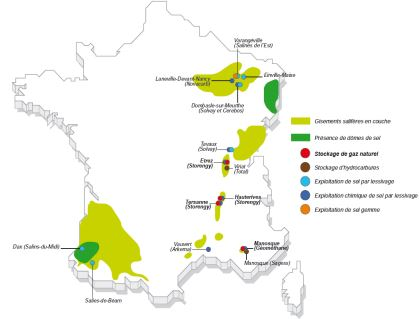
\includegraphics[width=.85\linewidth]{image/chap4/IV.4.ii.jpg}
\captionof{figure}{Couches géologiques de sel en France \cite{Hadj_Hassen_Jallais_2020}}
\label{fig:carteSelFrance}
\end{center}

Le sel se forme par évaporation des sels contenus dans l’eau de mers existant il y a plusieurs millions d’années. Il peut être présent sous forme de diapirs ou de couches.
La principale difficulté réside donc dans le fait que le sel n’est pas présent partout en France. Il n’est concentré que dans certaines régions, comme en témoigne la carte ci-contre (figure ~\ref{fig:carteSelFrance}) \cite{Hadj_Hassen_Jallais_2020}.

Les principales zones de recherches sont donc le Bassin Aquitain, la vallée du Rhône, le bassin Rhénan et l’Alsace-Lorraine. 
La deuxième difficulté est la profondeur de la couche de sel et l’épaisseur de celle-ci. Pour creuser une cavité saline qui respecte les critères choisis, l’idéal serait de trouver du sel atteignant des profondeurs de l’ordre de 1000 mètres et 
une épaisseur de quelques centaines de mètres.

Les recherches menées à l’aide du site Infoterre et de coupes géologiques nous ont permis de sélectionner 5 sites pouvant accueillir des cavités salines (ceux-ci sont présentés en détail dans l'annexe M) : 
\begin{itemize}
\item Sites de Dax et Gaujacq : le stockage est intéressant car l’épaisseur de la couche de sel à cet endroit semble être assez importante.
\item Site de Manosque : ce site contient déjà des infrastructures de stockage d’hydrocarbures, ce qui rend facile l’installation de cavités d’hydrogène.
\item Site de Hauterives : il est à noter que le sel de cette partie de la France est très fluant, mais la capacité de la région à accueillir de l’hydrogène semble prometteuse.
\item Site de Mackenheim : l’épaisseur de la couche à cet endroit est plus faible que pour les autres, mais cela reste intéressant dans une optique d’ouverture sur le marché européen.
\end{itemize}


Ces sites ont été choisis en fonction des critères définis en amont. Les sites choisis sont résumés sur la carte montrée à la figure ~\ref{fig:carteResumee}.

Les sites choisis ont été reliés à une configuration pour alimenter en hydrogène les zones d’intérêt. Hauterives a par exemple été choisi pour incarner la configuration 1 et alimenter Lyon en hydrogène dans l’optique du scénario P2M. 

\end{multicols}

\subsubsection{Choix de sites potentiels pour les cavités minées}
Les zones de recherche sont celles présentant des roches compétentes principalement du granite et du calcaire et à bonne profondeur, dans notre cas 100 m.
Parmis la liste de 8 sites retenus, nous présentons ici un en particulier qui correspond à la configuration 2.

\begin{figure}[!h]
\centering
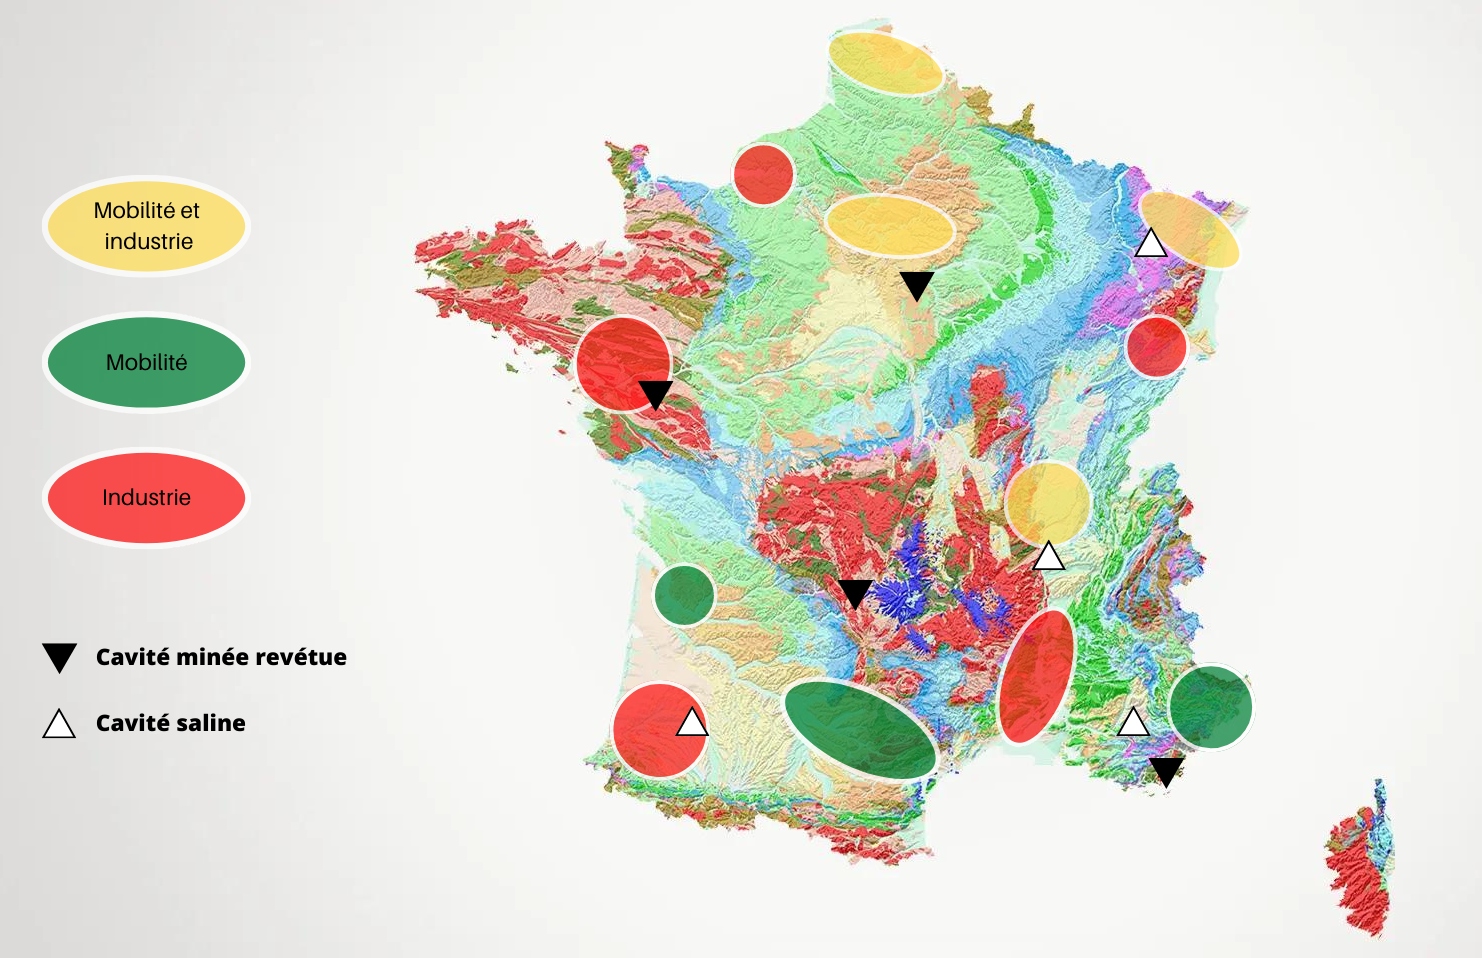
\includegraphics[width=.8\linewidth]{image/chap4/Mobilité et industrie recadré.PNG}
\caption{Résumé des sites retenus. Source: carte de France Hydrogène\hyperref[sec:presRef]{[I]} et carte géologique BRGM\cite{InfoTerreCarte}}
\label{fig:carteResumee}
\end{figure}


\subsubsection{Choix des sites pour le stockage liquide}
La particularité du stockage liquide est qu’il ne nécessite pas de grandes profondeurs (engendrant donc des coûts moins élevés) et que les cavités sont plus petites. 
Nous nous sommes alors intéressés à des régions où nous n’avions pas encore sélectionné de sites, afin de pallier le manque. Par exemple, la région du Havre était signalée par France Hydrogène comme une zone à besoin. Dans cette ville, il existe des zones composées de craie, à une profondeur de 3 mètres. Nous avons également cherché à placer un réservoir en Normandie, région laissée de côté jusqu’alors. Le granite d’Avranches s’est avéré très pertinent car il n’est pas profond.
Paris est également une ville pour laquelle les cavités enterrées et le stockage liquide sont intéressants. En effet, la mobilité parisienne est très développée et nécessite donc de l’hydrogène pour alimenter les transports en commun. En se plaçant à Boulogne, on trouve du calcaire à 3 m de profondeur, ce qui est intéressant. 
Nous avons aussi retenu le granite de Grézieu-la-Varenne, près de Lyon, pour les mêmes raisons de profondeur. Les détails des sites géologiques sont présentés en annexe M.







\section{Chapitre V : Bilan économique}
Dans les chapitres précédents, sept principales configurations de stockage en cavités salines, minées et réservoirs enterrés ont été identifiées par rapport aux applications possibles de l'hydrogène produit par électrolyse de l’eau ou vaporeformage.

L’objectif de ce dernier chapitre est d’approfondir l’étude de ces configurations en réalisant une étude économique simple, prenant en compte les coûts générés sur 30 ans. La finalité de ce propos visera une conclusion sur la faisabilité des différents projets, incluant leur rentabilité et de les comparer à d’autres techniques de stockage déjà existantes.

\subsection{Flux monétaires}

Toute activité industrielle est accompagnée de flux monétaires, dont le résultat annuel est appelé “cash-flow”. Ces flux de trésorerie sont divisés en 2 parties : 
\begin{itemize}
\item Flux entrants ou recettes d’exploitations. Ce sont des flux positifs.
\item Flux sortants ou dépenses.
\end{itemize}
Notre évaluation économique est basée sur un modèle simple dans lequel les dépenses ont été divisées en deux parties : 
\begin{itemize}
\item Dépenses d'investissement et de renouvellement (CAPEX)
\item Dépenses opératoires (OPEX)
\end{itemize}
De plus, dans l'analyse économique d'un projet, il faut tenir compte des fluctuations de la valeur de la monnaie, qui sont décrites par deux grandeurs : l'inflation (i) et le taux d'intérêt d'un placement ($\tau$). 

\subsubsection{Evaluation des CAPEX}
Les coûts retenus pour les infrastructures diffèrent d'une configuration à l'autre en fonction de l'application industrielle envisagée (P2I ou P2M), mais aussi en fonction du type de cavité de stockage, du type de transport et des moyens de production.  Les CAPEX calculés pour les 7 infrastructures comprennent leur achat et leur installation (cf. figure 32).  
Pour évaluer les investissements initiaux nécessaires à la phase de conditionnement, nous nous sommes appuyés sur des simulations réalisées avec le logiciel \emph{ASPEN PLUS}, et avons implémenté les schémas de conditionnement donnés précédement. Les données récoltées sont résumées dans la figure 32 (exemple pour la configuration 1):

\begin{figure}[h!]
\centering
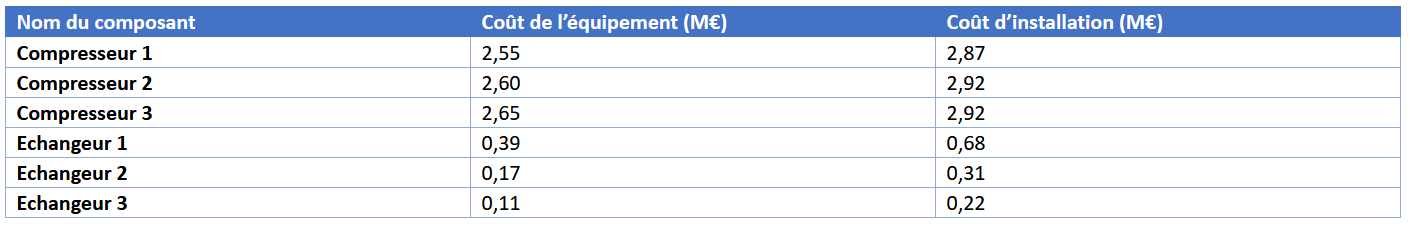
\includegraphics[width=0.9\linewidth]{image/chap5/Tableau 1 chap 5.png}
\caption{Résumé des coûts de conditionnement de la configuration 1. }
\end{figure}

Pour les coûts liés à la création de cavités minées revêtues, nous nous sommes appuyés sur les données du projet ayant eu lieu à Skallen en Suède précisées en Annexe N. Aussi nous prendrons comme coût de la cavité saline 100 €/m3, d’après des données proposées par Storengy (cf. Annexe N). 

Les coûts des installations de génie civil et leur gestion ont également été pris en compte (20 \% du CAPEX initial) et les données que nous avons utilisées pour évaluer les coûts liés au transport ainsi que les prix des matériaux qui interviennent dans nos différentes configurations sont précisés en Annexe L. 

En ce qui concerne le transport de l’hydrogène, le prix des pipelines étant de 1 M€/km, ce qui représente un coût faramineux pour le producteur d’hydrogène, nous avons décidé de considérer que le coût lié aux pipelines serait assumé par l’état ou l’union européenne. Pour les transports par camion, bien que les distances entre les sites de stockage et d’utilisation soient différentes en fonction des configurations, nous allons les considérer identiques et égales à 100 km (dans un souci de comparaison).
De plus, la durée de vie des appareils nous permet de prévoir le nombre de remplacements afin de calculer le CAPEX de renouvellement sur 30 ans. Nous pouvons ainsi comparer la part des différents appareils dans le CAPEX total sur 30 ans (cf. figure 33).

\begin{figure}[h!]
\centering
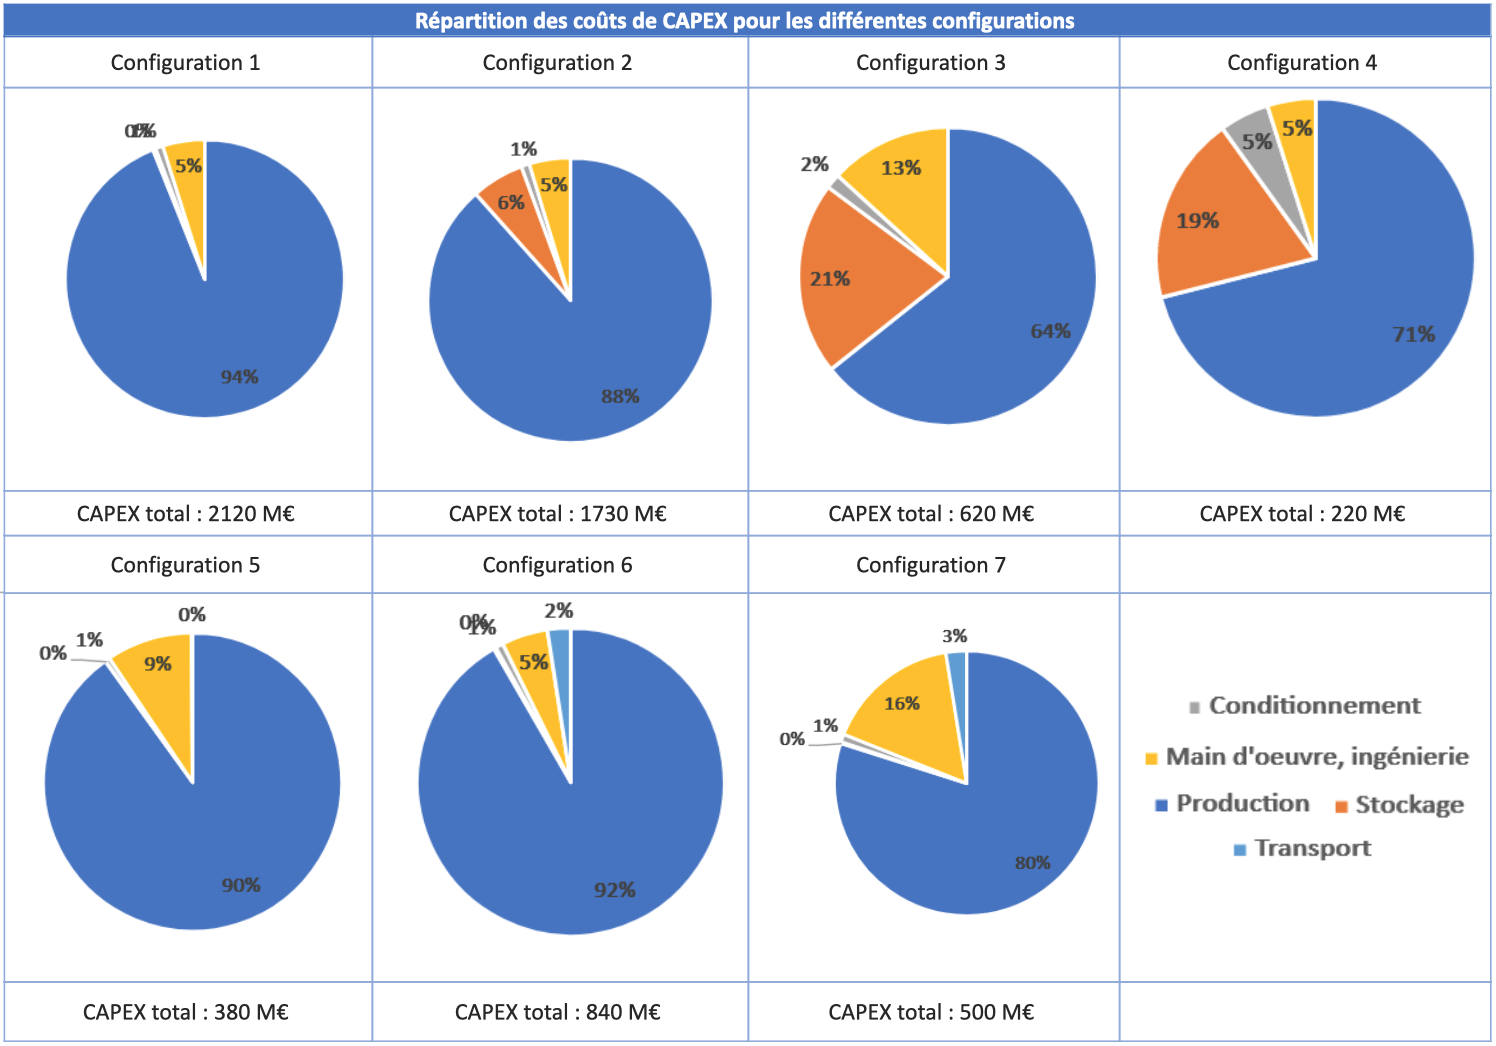
\includegraphics[width=0.9\linewidth]{image/chap5/Tableau 2 chap 5.png}
\caption{Résumé des CAPEX des différentes configurations.}
\end{figure}

On remarque que la majorité du coût se concentre sur la production par SMR ou électrolyse. En effet, ces procédés sont chers et les électrolyseurs doivent être renouvelés tous les 7-8 ans, soit 4 fois sur 30 ans.  
Pour les 4 scénarios en P2M (C1, C2, C5 et C6) on remarque des comportements similaires.  
Néanmoins, on remarque que dans l'ensemble des configurations, le conditionnement représente une part faible des CAPEX.

De plus, le coût d’un électrolyseur par rapport à une station SMR est bien 2 à 3 fois plus cher d’après nos calculs, ce qui correspond à la réalité du marché.


\subsubsection{Evaluation des OPEX}

Les coûts annuels considérés sont principalement le coût de l’électricité dans les phases de production et de conditionnement, auxquels nous avons ajouté les salaires, que nous avons estimés à 15\% du CAPEX d’investissement. La figure 34 résume les OPEX annuels pour chaque configuration.


\begin{figure}[h!]
\centering
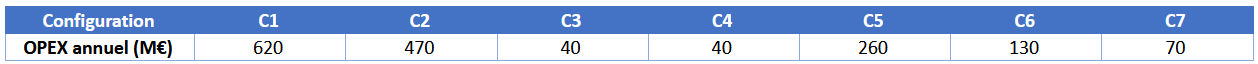
\includegraphics[width=0.9\linewidth]{image/chap5/Tableau 3 chap 5.png}
\caption{Résumé des OPEX des différentes configurations. }
\end{figure}

Afin de déterminer le prix de l’électricité de la partie conditionnement, nous avons, à l’aide du logiciel \emph{ASPEN PLUS}, déterminé les puissances de chaque composant en multipliant la variation d’enthalpie à chaque étape et le débit considéré. Puis, dans une démarche de transition énergétique, nous avons utilisé le prix de l’électricité verte en France.

En général, l’eau utilisée dans les échangeurs est directement puisée dans les nappes phréatiques, nous avons négligé le prix de l’eau devant celui de l’électricité. On retiendra que le prix de l’électricité de l’électrolyseur est très important par rapport au reste des coûts annuels.  

\subsubsection{Flux entrants : évaluation des recettes}
Concernant les recettes, nous avons uniquement considéré celles dues à la vente de l’hydrogène, sous forme liquide ou gazeuse. Pour l’application industrielle, nous avons fixé un prix de l'hydrogène de 5 €/kg pour l'industrie, et pour la mobilité, un prix de 14 €/kg \hyperref[sec:presRef]{[VII]}.
Nous avons décidé de ne pas prendre en compte la valorisation de capacité de stockage, c’est-à-dire la potentielle prime gouvernementale attribuée pour des capacités de stockage d’énergie verte. Cela ne gêne pas notre étude car cette dernière est comparative.
Pour les scénarios utilisant la technique de production SMR, il est impératif d’utiliser une cellule CCS pour capter le carbone rejeté mais cela entraîne un coût important (en CAPEX et en OPEX). Ce coût est en réalité amorti par la taxe carbone (taxe environnementale sur les émissions de $CO_2$) non prise en compte dans notre étude.

\subsubsection{Actualisation et cash-flows}
Le cash-flow se définit comme le résultat annuel des flux monétaires de l'entreprise. 
Celui à l'année p est défini comme : $$CF_p = R_p - CO_p - I_p $$ avec $R_p$ les recettes ; $CO_p$ les coûts opératoires directs ; $I_p$ l'investissement de l'année p.

Des quantités d'argent reliées à des années différentes ne sont pas comparables. Il est donc nécessaire de ramener toutes les sommes d'argent manipulées à la valeur qu'elles auraient aujourd'hui. La notion de cash flow actualisé de l'année p est définie comme : $$ CF^a_p = \frac{R_p - CO_p - I_p}{(1+a)^p} $$ où $ a = \tau - i $ s'appelle le taux d'actualisation.

Nous avons ainsi calculé, sur 30 ans, les cash-flows pour chacune des configurations ainsi que les cash-flows actualisés.  
Ces données vont nous permettre d’étudier par la suite la rentabilité de notre projet.  


\subsection{Rentabilité du projet}

Il existe des critères simples pour évaluer économiquement un projet d'une durée de N années. 
La création de richesse peut se mesurer par sa valeur nette actualisée, notée VAN :
$$ VAN = \sum_{p=0}^{N} CF^a_p = \sum_{p=0}^{N} \frac{R_p - CO_p - I_p}{(1+a)^p} $$

La VAN s'interprète comme le supplément de richesse amenée par le projet par rapport à un placement en banque de l'investissement initial au taux a.

Pour quantifier la rentabilité d'un projet, il est possible s'intéresser au taux de rentabilité interne, noté TRI.  

Le taux d'actualisation à imposer tel qu'un placement au taux a soit équivalent au projet industriel est par définition le TRI.

$$ \sum_{p=0}^{N} \frac{R_p - CO_p - I_p}{(1+TRI)^p} = 0 $$

\begin{figure}[h!]
\centering
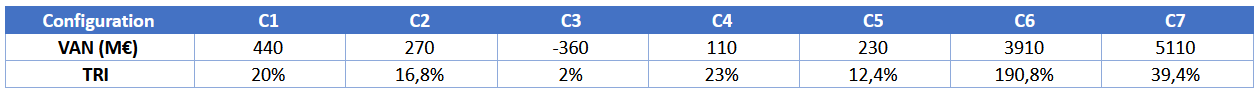
\includegraphics[width=0.9\linewidth]{image/chap5/Tableau 4 chap 5.png}
\caption{ Récapitulatif des VAN et TRI pour toutes les configurations. }
\end{figure}

Afin de comparer les configurations 1 et 2, on divise le TRI et la VAN par la capacité d’Hydrogène produite, on obtient un TRI normalisé de 6,7\% pour la configuration 1 et de 7,3\% pour la configuration 2, et une VAN normalisée de 1,46 pour la première et de 1,17 pour la seconde. On en conclut donc que la configuration 1 est plus rentable, et donc qu’il est préférable de stocker l'hydrogène en cavité saline lorsque cela est possible. Néanmoins, comme évoqué au chapitre IV, le sel n’est pas présent partout en France, d’où la nécessité d’utiliser des cavités minées.  

La comparaison des configurations 2 et 6 nous amène à penser que le stockage de l’Hydrogène sous forme liquide est bien plus rentable que sous forme gazeuse. 

Pour comparer les configurations 4 et 7, deux paramètres sont modifiés : l’état de l’Hydrogène et le type de production. Nous savons de la comparaison précédente qu’il est bien plus avantageux de stocker en liquide qu’en gazeux l’hydrogène, or ici la configuration 7 a un meilleur TRI que la configuration 4 mais l’écart est moindre, on en déduit donc que la production par vaporeformage du méthane est plus économique que l’électrolyse, il ne faut en revanche pas oublier que cette méthode est bien plus polluante que la seconde (car émettrice de $CO_2$) 

En ce qui concerne les configurations 5 et 6, si on ramène à la tonne d’hydrogène produit, on obtient un TRI de 2,4\% pour le réservoir enterré et 1\% pour les cavités minées revêtues. Ainsi, d’après nos calculs et avec les hypothèses faites, nous trouvons que les réservoirs enterrés semblent plus rentables que les cavités minées revêtues. Une explication possible peut être liée au fait que les réservoirs enterrés ont besoin d’être à des profondeurs bien inférieures.  

Enfin, on remarque que la technique de vaporeformage puis stockage en cavité saline pour l’industrie (scénario 3) ne semble pas optimale : le TRI est bas et la VAN négative, ce qui veut dire qu’on aurait gagné plus d’argent si l’investissement initial avait été placé en banque. Soyons néanmoins vigilants avec cette conclusion car quelques recettes compensatoires n’ont pas été prises en compte ici. 





\phantomsection
\section*{Conclusion}  \addcontentsline{toc}{section}{Conclusion}

\phantomsection
L'hydrogène est un vecteur énergétique qui permettrait la décarbonation de différents procédés. Nous avons présenté dans cette étude deux utilisations de l'hydrogène: une utilisation Power to Mobility
et une utilisation Power to Industry. Nous avons volontairement écarté une utilisation Power to Power qui ne représenterait qu'une économie de niche sous l'hypothèse d'une énergie décarbonnée disponible à profusion. Utiliser l'hydrogène dans les transports ou dans l'industrie présente de nombreux défis techniques et sociétaux. 
Il faut produire, stocker et distribuer l'hydrogène en prenant en compte les aspects environnementaux des procédés et de la viabilité économique des procédés.

Concernant les ambitions européennes et françaises autour de l'hydrogène, l'UE souhaite produire 10 millions de tonnes d'hydrogène et en importer autant à l'horizon 2030. La France souhaite installer 6,5GW d'électrolyseurs dans un plan d'investissement de 30 milliards d'euros pour devenir le leader de l'hydrogène vert en 2030.


Différentes méthodes de stockage  ont été retenues en fonction de l'utilisation de l'hydrogène et de son état (gazeux ou liquide). 
Il est plus intéressant de transporter et stocker l'hydrogène sous forme liquide puisqu'il contient la même énergie dans un volume beaucoup plus faible comparé à l'état gazeux. 
L'hydrogène liquide peut être stocké soit dans des reservoirs enterrés, soit dans des cavités minées revêtues. Limiter la propagation du froid constitue le principal enjeu du stockage liquide et l'isolant thermique retenu est la perlite. Il n'est pas nécessaire  de comprimer l'hydrogène liquide, on évite ainsi d'avoir à creuser aussi profond que dans le cas gazeux. Cela est donc intéressant économiquement. Cependant, il peut être nécessaire de drainer l'eau contenue dans les roches environnantes afin d'éviter l'endommagement de la cavité. Le choix entre cavité minée revêtue et réservoir enterré dépend essentiellement de l'application que l'on souhaite faire de l'hydrogène.
L'hydrogène gazeux peut être stocké en cavité saline ou minée revêtue. Il semble plus pertinant de privilégier les cavités salines, si possible, puisqu'elles restent plus simples à créer, même si cela peut prendre plusieurs années. Le sel présente également l'avantage d'être naturellement étanche : pas besoin d'isolant ou de béton armé. Enfin, il n'est souvent pas nécessaire de construire plusieurs cavités salines, on évite ainsi les problématiques liées à la distance minimale de sécurité entre les cavités.

L'hydrogène n'est pas présent à l'état naturel et il faut donc le produire en apportant de l'énergie de l'extérieur. Nous avons étudié deux méthodes de production de l'hydrogène: le vaporeformage couplé au captage de $CO_2$ et l'électrolyse. 96\% de l'hydrogène est produit par vaporeformage actuellement. Cette technique utilise du gaz naturel. On casse les liaisons carbone-hydrogène en chauffant à 760°C. Le vaporeformage couplé à une captation de $CO_2$ est émetteur de $CO_2$ à hauteur de $550g $ pour $1kg$ de $H_2$ dans le meilleur des cas. Le vaporeformage présente néanmoins un intérêt économique certain. La production d'hydrogène par vaporeformage est bien connue des industriels. On peut aussi synthétiser de l'hydrogène par électrolyse de l'eau et c'est cette technique qui est mise en avant dans les rapports et publications gouvernementaux. Nous avons retenu ce type d'électrolyseurs car ils présentent un temps de réponse très faible et le plus grand débit de production d'hydrogène parmi les technologies d'électrolyse. L'électrolyse a cependant un rendement de l'ordre de $62\%$. Il faut un apport très conséquent d'électricité décarbonée ($55kWh/kg H_2$), ce qui représente un véritable défi. Après production, il faut conditionner l'hydrogène pour son transport ou son utilisation. On peut penser à le liquéfier ou le comprimer à très haute pression. Liquide, l'hydrogène a un pouvoir calorifique 4 fois moins grand que l'essence mais 780 fois plus grand que l'hydrogène gazeux à pression atmosphérique. Pour liquéfier l'hydrogène, il faut le refroidir en dessous de 20,3K à pression atmosphérique en prenant en compte la réaction de conversion ortho-parahydrogène fortement exothermique. Comprimer l'hydrogène est aussi une solution pour augmenter sa densité énergétique mais il faut considérer des alliages spéciaux dans les outils de stockage pour supporter les hautes pressions. Transporter l'hydrogène sous forme de gaz fait apparaître des problèmes de pertes de charges dans les conduites et donc des pertes énergétiques. Transporter l'hydrogène sous forme liquide nécessite d'isoler thermiquement les réservoirs pour éviter les phénomènes de regazéification qui pourraient détruire les biens par surpression.

Nous avons considéré dans un quatrième temps les impacts environnementaux et sociétaux de l'hydrogène. L'hydrogène est fortement inflammable et détonnant ce qui nécessite des dispositifs de détection des fuites et de ventilation. C'est aussi un gaz à fort effet de serre : 11 fois plus important que le méthane. Les installations de stockage de l'hydrogène peuvent ainsi être classées \textit{SEVESO} au même titre que les installations de stockage de gaz naturel. D'un point de vue sociétal, il semblerait que le public soit relativement favorable au développement de la filière hydrogène et dénonce peu les risques écologiques. L'hydrogène n'est pas perçu comme un vecteur énergétique dominant dans le mix énergétique futur. Nous avons pu caractériser des sites de stockage \textit{ad hoc} en fonction de la géologie française.

Dans une démarche complète d’étude de faisabilité s’insère l’étude économique du projet. Cette étude converge avec les nombreux constats effectués dans chacune des parties. En effet, en prenant en compte les études faites sur les TRI et VAN de chaque configuration on remarque que la mise en place de cavités salines est plus rentable que les cavités minées revêtues. Aussi, stocker l’hydrogène sous forme liquide est bien plus rentable, même si cela n'est pas compatible avec une mise en place de cavités salines. En omettant l’aspect environnemental du procédé, il est clair qu’un investisseur préfèrera la production par vaporeformage avec captation de $CO_2$ plutôt que par électrolyse. Néanmoins, dans une problématique de développement durable il faut encourager la production d’hydrogène par électrolyse alimentée en électricité verte. 
Ainsi, dans une optique de stockage d’hydrogène liquide produit par électrolyse, si l’on veut réduire les couts, il est préférable de stocker l’hydrogène dans des réservoir enterrées plutôt que des cavités minées revêtues. 
Cependant, les coûts sont faramineux, et il apparait clairement que sans subventions de l’Etat par divers moyens (valorisation des capacités de stockages, aide …) la mise en place de solutions par hydrogène semblent compliquées.

In fine, le développement de la filière hydrogène en France pour décarbonner des procédés nécessite de surmonter maints défis techniques dans sa production, son transport et son stockage. Au regard de notre rapport, l'hydrogène peut s'inscrire dans la transition énergétique mais ne sera pour autant pas prédominant dans le mix énergétique final. Si l'hydrogène devait devenir un vecteur énergétique bas-carbone, c'est avant tout sous l'hypothèse d'une énergie primaire elle aussi bas-carbone. La production d'énergie primaire décarbonnée est donc l'objectif principal de ces prochaines années. 


\newpage

%début des annexes
\backmatter

\phantomsection
\section*{Annexes} \addcontentsline{toc}{section}{Annexes}

\subsection*{Tableau de bord de la première semaine}\addcontentsline{toc}{subsection}{Tableau de bord}
La première semaine a été consacrée à des visites d'entreprise afin de mieux connaître le sujet de l'hydrogène.

Lors de la première journée,  après un rapide rappel des objectifs du MIG, nous avons assisté à une conférence de France Hydrogène pendant la fin de matinée. Cette conférence était utile pour nous présenter le marché actuel du dihydrogène en France et dans le monde, les intérêts de cette molécule et les enjeux techniques et économiques liés à celle-ci. 
Nous avons ensuite enchaîné sur une visite de Elogen l’après-midi, qui est le premier fabriquant d’électrolyseur en France : cela nous a permis d‘apprendre les procédés techniques concrets qui servent à la production d’hydrogène vert et des précisions utiles sur les défis et les enjeux environnementaux, techniques et économiques liés à ce mode de production. 

Durant la deuxième journée, nous nous sommes rendus aux laboratoires d’Engie. Ils ont pu nous présenter leurs projets liés au dihydrogène, en particulier à la liquéfaction de cette molécule. Ce processus nous a été décrit comme complexe et coûteux par un ingénieur de recherche et un chef de projet de cette entreprise, qui nous ont ensuite fait visiter leurs installations de laboratoire. Nous avons pu ainsi mieux comprendre la complexité de la liquéfaction de l’hydrogène et les processus déjà existants, ainsi que les perspectives d’améliorations futurs de ceux-ci.

Pendant la troisième journée, nous sommes allés sur les sites de Air Liquide. Ils ont utilisé la matinée pour nous présenter leur entreprise ainsi que pour nous décrire la méthode de production de dihydrogène la plus utilisée actuellement, qui est le vaporeformage du méthane. Nous avons ensuite démarré l’après-midi par une visite de leurs deux stations à hydrogène, qui permettent d’alimenter un réseau de bus et un réseau de taxi et nous avons ensuite enchaîné sur des présentations qui portaient sur les enjeux liés à la sécurité dans le maniement de l’hydrogène gazeux, certains procédés de stockage souterrain de l’hydrogène et enfin les procédés de captation et de valorisation du CO2 émis après vaporeformage du méthane. 
\begin{center}
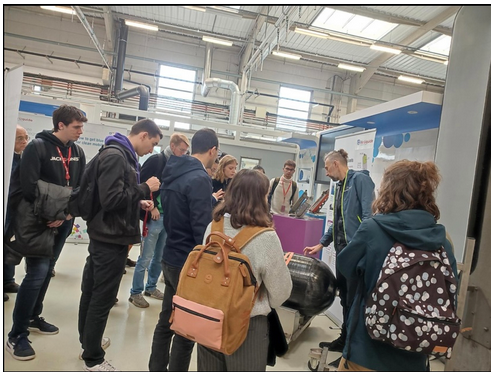
\includegraphics[width=0.5\linewidth]{image/annexe/tab_bord1.png}
\end{center}


A l’occasion de la quatrième journée, nous avons passé la matinée à nous familiariser avec les études bibliographiques afin de nous aider dans nos futures recherches documentaires. Puis, l’après-midi a été consacré aux différentes présentations de Geostock, un des principaux acteurs mondiaux de stockage de gaz, qui nous a décrit les différentes technologies de stockage du dihydrogène gazeux, les cavités salines et les cavités minées, revêtues ou non.

Enfin, nous avons consacré la cinquième journée à la visite d’un site de stockage de gaz de Storengy, autre acteur majeur du stockage de gaz en France, à Bourg-en-Bresse. Après une présentation de l’entreprise et des techniques de stockage de gaz, nous avons ainsi pu voir de nos propres yeux plusieurs installations : compresseurs, détendeur, centre de contrôle… Cette visite avait l’utilité de nous rapprocher le plus possible du terrain et des opérations sur place. Là aussi, les enjeux économiques et techniques liés au stockage souterrain du dihydrogène gazeux pour les années à venir nous ont été décrits.
\begin{center}
\includegraphics[width=0.5\linewidth]{image/annexe/tab_bord2.png}
\end{center}

\subsection*{Annexe A: Configurations étudiées} \addcontentsline{toc}{subsection}{Annexe A: Configurations étudiées}

\begin{figure}[h]
\centering
\includegraphics[width=0.9\linewidth]{image/annexe/config_cavite_minee/configs.png}
\caption{Détail des configurations}
\end{figure}

\FloatBarrier
\subsection*{Annexe B: Détails des configurations étudiées} \addcontentsline{toc}{subsection}{Annexe B: Configurations des cavités minées}

\begin{figure}
\centering
\begin{minipage}{.5\textwidth}
  \centering
  \includegraphics[width=0.8\linewidth]{image/annexe/config_cavite_minee/c1.png}
  \captionof{figure}{Configuration 1 }
  \label{fig:test1}
\end{minipage}%
\begin{minipage}{.5\textwidth}
  \centering
  \includegraphics[width=0.7\linewidth]{image/annexe/config_cavite_minee/c2.png}
  \captionof{figure}{Configuration 2 }
  \label{fig:test2}
\end{minipage}
\end{figure}

\begin{figure}
\centering
\begin{minipage}{.5\textwidth}
  \centering
  \includegraphics[width=0.7\linewidth]{image/annexe/config_cavite_minee/c3.png}
  \captionof{figure}{Configuration 3 }
  \label{fig:test1}
\end{minipage}%
\begin{minipage}{.5\textwidth}
  \centering
  \includegraphics[width=0.8\linewidth]{image/annexe/config_cavite_minee/c4.png}
  \captionof{figure}{Configuration 4 }
  \label{fig:test2}
\end{minipage}
\end{figure}

\begin{figure}
\centering
\begin{minipage}{.5\textwidth}
  \centering
  \includegraphics[width=0.7\linewidth]{image/annexe/config_cavite_minee/c5.png}
  \captionof{figure}{Configuration 5 }
  \label{fig:test1}
\end{minipage}%
\begin{minipage}{.5\textwidth}
  \centering
  \includegraphics[width=0.8\linewidth]{image/annexe/config_cavite_minee/c6.png}
  \captionof{figure}{Configuration 6 }
  \label{fig:test2}
\end{minipage}
\end{figure}

\begin{figure}
\centering
\begin{minipage}{.5\textwidth}
  \centering
  \includegraphics[width=0.9\linewidth]{image/annexe/config_cavite_minee/c7.png}
  \captionof{figure}{Configuration 7 }
  \label{fig:test1}
\end{minipage}%
\begin{minipage}{.5\textwidth}
  \centering
  \includegraphics[width=0.9\linewidth]{image/annexe/config_cavite_minee/donnes.png}
  \captionof{figure}{Données }
  \label{fig:test2}
\end{minipage}
\end{figure}

\FloatBarrier
\subsection*{Annexe C : Dimensions du réservoir enterré}\addcontentsline{toc}{subsection}{Annexe C : Dimensions du réservoir enterré}

\begin{figure}[h]
\centering
\includegraphics[width=0.8\linewidth]{image/annexe/reservoir_ent/dimReservoir.png}
\caption{Dimensions exactes du réservoir enterré}
\end{figure}

\begin{figure}[h]
\centering
\includegraphics[width=.7\linewidth]{image/annexe/reservoir_ent/reservoir3D.png}
\caption{Schéma d'un réservoir enterré - Emad Jahangir}
\end{figure}

\FloatBarrier
\subsection*{Annexe D : Rhéologie des roches} \addcontentsline{toc}{subsection}{Annexe D : Rhéologie des roches}
Cette section présente le détail des essais réalisés en laboratoire afin de caractériser la rhéologie des roches utiles à l’étude de cavités. 
Les propriétés ainsi mesurées ont été implémentées dans le fichier input du logiciel DEMETER. 

\subsubsection*{Échantillons de roches}

L’éprouvette de roche doit être propre et normalisée afin de réaliser les essais nécessaires à sa caractérisation. 
Pour ce faire, plusieurs étapes entrent en jeu : 
\begin{itemize}
\item Carottage : On prélève un échantillon du sol à étudier à l’aide d’un carottier, pour obtenir un prélèvement tubulaire de la roche. Cet échantillon ainsi obtenu est envoyé dans des laboratoires spécialisés pour analyse. 
\item
Préparation de l’échantillon : l'échantillon est soumis à des opérations de carottage si besoin, de découpage et de rectification des faces pour préparer des éprouvettes normalisées par rapport au type d'essai à conduire (Figure ~\ref{fig:d1}). On définit l’élancement d’une éprouvette comme le rapport de sa hauteur sur son diamètre.
\end{itemize}

\begin{figure}[h]
\centering
\includegraphics[width=.8\linewidth]{image/annexe/annexe_D/D1.png}
\caption{Carottes de sel du laboratoire de Fontainebleau, et éprouvettes d’essais}
\label{fig:d1}
\end{figure}

\FloatBarrier

\subsubsection*{Mesure des propriétés physiques }
Sur chaque éprouvette préparée, on détermine généralement : 
\begin{itemize}
\item La masse volumique par pesée et mesure du volume de l’échantillon dans son état initial,
\item La vitesse du son par mesure du temps de propagation que met une onde de compression pour traverser l'échantillon. Celle-ci permet de caractériser l’homogénéité du matériau en question. 
\end{itemize}
 
Pour le sel on trouve une masse volumique d’environ $2200 kg/m^3$ et une vitesse de son de l'ordre de 4500 m/s. 


\paragraph{Essai brésilien }

Pour faire un essai de traction de manière directe il faudrait réussir à « tirer » l’échantillon avec des pinces de traction. Cette méthode fonctionne pour des matériaux résistants à la traction mais le sel y est très sensible. C’est pour cela qu’on réalise cet essai de manière indirecte, c’est à dire que l’on prend un échantillon d’élancement 0,5 que l’on vient compresser diamétralement en créant ainsi une traction le long du diamètre perpendiculaire (Figure ~\ref{fig:d2})

\begin{figure}[h]
\centering
\includegraphics[width=.5\linewidth]{image/annexe/annexe_D/D2.png}
\caption{Essai de traction indirecte en laboratoire (essai brésilien)}
\label{fig:d2}
\end{figure}

\FloatBarrier
On en déduit la résistance à la traction que l’on définit comme la contrainte horizontale lors de la rupture : 
$$Rt = (F/ \pi RH)$$
 
avec : 
\begin{itemize}
\item Rt , la résistance à la traction 
\item F, l’effort fourni par la presse à la rupture 
\item R et H respectivement le rayon et la hauteur de l’éprouvette. 
\end{itemize}

Dans le cas du sel, on trouve une valeur d’environ 1,5MPa. Pour des raisons de sécurité, nous avons décidé de prendre une résistance à la traction nulle comme critère de stabilité des cavités. 


\paragraph{Essai de compression : cisaillement indirect }

Les essais de compression sont réalisés avec des éprouvettes d’élancement 2 pour éviter tout effet de flambage.

\begin{figure}[h]
\centering
\includegraphics[width=.3\linewidth]{image/annexe/annexe_D/D3.png}
\caption{Flambage de la roche lors d’un essai de compression}
\label{fig:d3}
\end{figure}
\FloatBarrier

Les essais de compression peuvent être simples ou triaxiaux et permettent de mesurer les paramètres élastiques à travers des cycles charge/décharge : le module de Young et le coefficient de Poisson.   

L’essai uni-axial est appelé essai de compression simple. On place l’éprouvette sous une presse et on lui applique une contrainte longitudinale %σ jusqu’à sa rupture. 

\begin{figure}[h]
\centering
\includegraphics[width=.3\linewidth]{image/annexe/annexe_D/D4.png}
\caption{Schéma d’un essai de compression simple }
\label{fig:d4}
\end{figure}
\FloatBarrier
                         
Les déformations longitudinales et transversales de la roche sont définies respectivement comme : 
  
$$\epsilon _l = \frac{\Delta l}{l_0} \; \textrm{  et  } \; \epsilon _t=\frac{\Delta b}{b_0}= \nu \epsilon _l $$  
 avec $\nu$ le coefficient de poisson 

Dans sa zone élastique, la roche suit la loi de Hooke $\sigma =\epsilon _l E$, ou E représente le module d’Young du matériau (en pascals)

\begin{figure}[h]
\centering
\includegraphics[width=.45\linewidth]{image/annexe/annexe_D/D5.png}
\caption{Graphique de comportement de la roche lors de l’essai de compression }
\label{fig:d5}
\end{figure}
\FloatBarrier

Plusieurs techniques sont utilisées pour accéder au coefficient de poisson et au module d’Young, la plus courante étant les jauges de déformations. 
Au cours d’un essai de compression triaxiale, l’éprouvette est placée dans une cellule cylindrique (Figure ~\ref{fig:d6}). L’espace entre les parois de la cellule et l’éprouvette, isolée par une jaquette en silastène, est rempli d’huile qui, une fois pressurisée, assure une pression latérale constante sur l’éprouvette (pression de confinement). Le maintien de la pression latérale est assuré par un générateur de pression à volume contrôlé qui permet de mesurer la variation du volume d’huile dans la cellule pendant toute la durée de l’essai. Cette variation du volume d’huile à une pression de confinement constante permet de calculer la variation du volume de l’éprouvette. 

\begin{figure}[h]
\centering
\includegraphics[width=.4\linewidth]{image/annexe/annexe_D/D6.png}
\caption{Cellule triaxiale au laboratoire du centre de Géosciences }
\label{fig:d6}
\end{figure}
\FloatBarrier

Dans le cas de l’essai triaxial, avec une pression de confinement P constante et une pression axiale Q, le déviateur de contraintes s’écrit : q = Q-P
Les essais de compression triaxiale permettent d'accéder à l'endommagement du sel via le déviateur dilatant qd. Ce dernier correspond à la valeur du déviateur à partir duquel le comportement de l'éprouvette n'est plus contractant. La Figure ~\ref{fig:d7} illustre les résultats d'un essai triaxial (à droite la contrainte axiale en fonction de la déformation longitudinale et à gauche le déviateur en fonction de la variation volumique). 
Le déviateur dilatant augmente avec la pression de confinement appliqué. Le critère de dilatance est souvent exprimé par une relation entre le déviateur dilatant et la pression moyenne (Figure ~\ref{fig:d8})

\begin{figure}[h]
\centering
\includegraphics[width=.4\linewidth]{image/annexe/annexe_D/D7.png}
\caption{Résultats d'un essai de compression triaxiale (en bleu : déformations globales mesurées par un capteur inductif et par variation de volume d'huile, en rouge: déformations locales mesurées par jauges)}
\label{fig:d7}
\end{figure}

\begin{figure}[h]
\centering
\includegraphics[width=.4\linewidth]{image/annexe/annexe_D/D8.png}
\caption{Exemples de critères de dilatance sur différents sels (Labaune et al., 2017)}
\label{fig:d8}
\end{figure}
\FloatBarrier

Nous avons simplifié la relation en adoptant un critère de dilatance relation linéaire : et en fixant des valeurs moyennes de a = 1.3 et b = 2.5 (en MPa). 
\paragraph{Essai de cisaillement}

L’essai a pour objet de mesurer les caractéristiques de rupture d’un échantillon de sol soumis à un cisaillement direct selon un plan imposé, à une vitesse constante. De cet essai peuvent être déduites les valeurs de l’angle de frottement $\phi$ et la cohésion C. 

L’essai s’effectue sur une éprouvette de sol placée dans un bâti de cisaillement constitué de deux demi boîtes indépendantes. Le plan de séparation des deux demi boîtes constitue un plan de glissement préférentiel correspondant au plan de cisaillement de l’éprouvette.
L’essai consiste à : 
\begin{itemize}
\item Consolider l’éprouvette de section s dans une première phase en appliquant sur la face supérieure un effort vertical constant maintenu pendant tout l’essai (contrainte $\sigma n=N/s$)
\item La phase de consolidation permet de calculer la vitesse à laquelle doit être cisaillé l’échantillon.
\item Cisailler ensuite le long du plan de séparation des 2 demi-boîtes en leur imposant un déplacement relatif à vitesse constante.
\item L’effort de cisaillement horizontal (T) est mesuré et la contrainte   $\tau=T/s$ est calculée.
\end{itemize}

\begin{figure}[h]
\centering
\includegraphics[width=.7\linewidth]{image/annexe/annexe_D/D9.png}
\caption{Essai de cisaillement en laboratoire}
\label{fig:d9}
\end{figure}
\FloatBarrier


La figure ~\ref{fig:d10} montre des courbes expérimentales d'un essai de cisaillement direct 

\begin{figure}[h]
\centering
\includegraphics[width=.7\linewidth]{image/annexe/annexe_D/D10.png}
\caption{Courbe contrainte-déformation d’un essai de cisaillement direct}
\label{fig:d10}
\end{figure}
\FloatBarrier


On obtient ainsi les courbes de cisaillement effort- déformation et l’on peut en déduire les droites
($\tau ; \sigma n$) pour les valeurs à la rupture.
Il est alors simple de déterminer l’angle de frottement $\phi$ et la cohésion effective C, respectivement la pente et l’ordonnée à l’origine de ces droites.

\begin{figure}[h]
\centering
\includegraphics[width=.45\linewidth]{image/annexe/annexe_D/D11.png}
\caption{Critère de Coulomb dans le plan des contraintes ($\tau,\sigma_n$)}
\label{fig:d11}
\end{figure}
\FloatBarrier



\paragraph{Essai de fluage}


Pour les matériaux visqueux, dont le sel fait parti, leur déformation va dépendre du temps, c’est le phénomène de fluage.  

L’intensité de ce phénomène dépend à la fois de la contrainte et de la température à laquelle est effectuée l’essai. C’est pour cela qu’on réalise l'essai dans un laboratoire en sous-sol, où la température est contrôlée. Une éprouvette d’élancement deux est placée dans une cellule triaxale où lui sont imposées une pression axiale, une pression latérale et une température (Figure ~\ref{fig:d12}). Un essai a une durée typique de quelques mois, au cours de laquelle on fait varier par paliers le déviateur de contraintes et la température pour simuler les conditions réelles d’évolution du sel et où l’on mesure l’évolution de la déformation axiale de l’éprouvette. 

Il existe de nombreuses lois qui permettent de décrire le comportement du sel en fonction de la température, du temps, des contraintes de pression et du déviateur. Nous avons décidé d’utiliser la loi de Lemaître dans notre étude. (cf chapitre 2) 

La Figure ~\ref{fig:d13} donne un exemple d'essai de fluage réalisé au laboratoire du centre de Géosciences.
Pour caractériser le niveau de fluage d'un sel, on définit l'indice de fluage qui correspond à la déformation viscoplastique calculée en \% pour un déviateur de 10 MPa, un temps de 365 jours et une température T = 328 K. 
Dans notre étude, nous avons retenu pour le sel les paramètres suivants : $\alpha=0,3 ; \beta=3,24 ; K = 0,72MPa ; A=2500 \textrm{ et } Tr=30 \textrm{°C}$. Ces paramètres conduisent à un indice de fluage de l'ordre de 6 \%. Cet indice traduit un sel relativement fluant.
Le coefficient de dilatation thermique $\alpha th$ peut être mesuré à chaque changement de palier de température sous déviateur de contraintes nul, c'est à dire lorsque la déformation ne provient que de la dilatation thermique. Dans notre étude, nous avons retenu $\alpha th = 40 10-6 K-1$. Les autres paramètres thermiques retenus pour le sel, la conductivité thermique et la capacité thermique volumique, sont respectivement de 5,78Wm-1K-1 et de 2 MJm-3K-1.

\begin{figure}[h]
\centering
\includegraphics[width=.8\linewidth]{image/annexe/annexe_D/D12.png}
\caption{Dispositif pour la réalisation d'un essai de fluage multipaliers (centre de Géosciences)}
\label{fig:d12}
\end{figure}
\FloatBarrier

\begin{figure}[h]
\centering
\includegraphics[width=.8\linewidth]{image/annexe/annexe_D/D13.png}
\caption{Exemple d'ajustement d'un essai de fluage multipaliers par la loi de Lemaitre}
\label{fig:d13}
\end{figure}
\FloatBarrier


\FloatBarrier
\subsection*{Annexe E : Simulation des cavités salines et minées sur DEMETHER} \addcontentsline{toc}{subsection}{Annexe E : Simulation des cavités salines et minées sur DEMETHER}

Pour l'application à l'industrie avec stockage en cavité saline (configuration 3), on a utilisé les données d'entrée ci-dessous:

\begin{figure}[h]
  \centering
  \includegraphics[width=0.65\linewidth]{image/annexe/cav_sal/ind.png}
  \caption{Données d'entrée de la configuration 3}
  \end{figure}
\FloatBarrier
On a également modélisé des cavités salines qui stockeraient de l'hydrogène gazeux destiné à la mobilité (configuration 1). Pour cela, on a d'abord utilisé les données d'entrée suivantes:

\begin{figure}[h]
  \centering
  \includegraphics[width=0.65\linewidth]{image/annexe/cav_sal/p2mf.png}
  \caption{Données d'entrée de la configuration 1}
  \end{figure}
\FloatBarrier
Pour une cavité sphérique d'un rayon de 21 m, on obtient l'évolution de la pression suivante:
\begin{figure}[h]
  \centering
  \includegraphics[width=0.8\linewidth]{image/annexe/cav_sal/P2M_faux/P.png}
  \caption{Evolution de la pression (MPa)}
  \end{figure}
\FloatBarrier
On remarque que la pression n'est pas comprise entre la pression maximale et minimale, donc on en conclue que les données d'entrée aboutissent à une cavité pas stable. Par manque de temps, notre encadrante Laura Blanco Martín a fait les calculs qui nous ont permis d'obtenir une cavité sphérique stable. Le rayon devait valoir 25 mètres, et on observe qu'en effet la cavité obtenue avec cette donnée est bien satisfaisante.

  \begin{figure}[h!]
    \centering
    
    \begin{subfigure}[b]{0.4\linewidth}
        \includegraphics[width=\linewidth]{image/annexe/cav_sal/P2M_bon/P.png}
        \caption{Evolution de la pression (MPa).}
    \end{subfigure}
    \hspace{1cm}
    \begin{subfigure}[b]{0.4\linewidth}
        \includegraphics[width=\linewidth]{image/annexe/cav_sal/P2M_bon/P_zoom.png}
        \caption{Evolution de la pression zoomée (MPa)}
    \end{subfigure}
    
    \begin{subfigure}[b]{0.42\linewidth}
        \includegraphics[width=\linewidth]{image/annexe/cav_sal/P2M_bon/q(t).png}
        \caption{déviateur (MPa).}
    \end{subfigure}
    \begin{subfigure}[b]{0.42\linewidth}
        \includegraphics[width=\linewidth]{image/annexe/cav_sal/P2M_bon/M.png}
        \caption{masse (kg).}
    \end{subfigure}
    
    \begin{subfigure}[b]{0.42\linewidth}
        \includegraphics[width=\linewidth]{image/annexe/cav_sal/P2M_bon/T.png}
        \caption{température (ºC).}
    \end{subfigure}
    \begin{subfigure}[b]{0.42\linewidth}
        \includegraphics[width=\linewidth]{image/annexe/cav_sal/P2M_bon/Delta_vol_(1).png}
        \caption{Variation volumique (\%).}
    \end{subfigure}
    \caption{Evolution de la pression (MPa), déviateur (MPa), masse (kg), , température (ºC), variation volumique (\%). }
    
    \end{figure}
    
    \begin{figure}[h!]
    \centering
    
    \begin{subfigure}[b]{0.4\linewidth}
        \includegraphics[width=\linewidth]{image/annexe/cav_sal/P2M_bon/stt.png}
        \caption{Evolution de la contrainte orthoradiale (MPa).}
    \end{subfigure}
    \hspace{1cm}
    \begin{subfigure}[b]{0.4\linewidth}
        \includegraphics[width=\linewidth]{image/annexe/cav_sal/P2M_bon/stt_zoom.png}
        \caption{Evolution de la contrainte orthoradiale zoomée (MPa)}
    \end{subfigure}
    
    \begin{subfigure}[b]{0.42\linewidth}
        \includegraphics[width=\linewidth]{image/annexe/cav_sal/P2M_bon/szz.png}
        \caption{Evolution de la contrainte selon z (MPa).}
    \end{subfigure}
    \begin{subfigure}[b]{0.42\linewidth}
        \includegraphics[width=\linewidth]{image/annexe/cav_sal/P2M_bon/szz_zoom.png}
        \caption{Evolution de la contrainte selon z zoomée (MPa).}
    \end{subfigure}

    \caption{Evolution de la  contrainte orthoradiale (MPa) et contrainte selon z (MPa) au cours du temps dans la cavité}
    \label{fig:7 figures}
    \end{figure}
\FloatBarrier
Tous les critères dont on a parlé dans le paragraphe 2.3.1-B sont bien satisfaits. Cette cavité est bien réalisable.

Voici les résultats obtenus pour l’application du stockage en cavités minées à la mobilité (configuration 2).

\begin{figure}[h]
\centering
\includegraphics[width=.7\linewidth]{image/annexe/Simul_cav_minee/Cav_minée_GH2_P2M_pression.jpg}
    \caption{Evolution de la pression dans la cavité}
\end{figure}

\begin{figure}[h]
\centering
\includegraphics[width=.65\linewidth]{image/annexe/Simul_cav_minee/Cav_minée_GH2_P2M_temperature.jpg}
\caption{Evolution de la température}
\end{figure}

\begin{figure}[h]
\centering
\includegraphics[width=.65\linewidth]{image/annexe/Simul_cav_minee/Cav_minée_GH2_P2M_contrainte_orthoradiale.jpg}
\caption{Evolution de la contrainte orthoradiale}
\end{figure}

\begin{figure}[h]
\centering
\includegraphics[width=.65\linewidth]{image/annexe/Simul_cav_minee/Cav_minée_GH2_P2M_contrainte_axiale.jpg}
\caption{Evolution de la contrainte selon z (MPa)}
\end{figure}

\newpage
\FloatBarrier
\subsection*{Annexe F : Simulation numérique du réservoir enterré sur COMSOL}\addcontentsline{toc}{subsection}{Annexe F : Simulation numérique du réservoir enterré sur COMSOL}
  
\begin{figure}[h]
\centering
\includegraphics[width=.8\linewidth]{image/annexe/reservoir_ent/Annexe_2.png}
\caption{Schéma et dimensions d'une coupe}
\end{figure}
  
\begin{figure}[h]
\centering
\includegraphics[width=.8\linewidth]{image/annexe/reservoir_ent/Annexe_3.png}
\caption{Résultat de l'étude à température constante}
\end{figure}
  
\begin{figure}[h]
\centering
\includegraphics[width=.8\linewidth]{image/annexe/reservoir_ent/Annexe_4.png}
\caption{Résultat de l'étude à température variable}
\end{figure}
   
\begin{figure}[h]
\centering
\includegraphics[width=.8\linewidth]{image/annexe/reservoir_ent/Annexe_4_bis.png}
\caption{Résultats de l'étude à température pour d'autres épaisseurs}
\end{figure}
  
%\begin{figure}[!h]
%\centering
%\includegraphics[width=.8\linewidth]{image/annexe/reservoir_ent/Annexe_5.png}
%\caption{Résultat de l'étude à température variable pour une température moyenne plus faible}
%\end{figure}
  
\begin{figure}[!h]
\centering
\includegraphics[width=.8\linewidth]{image/annexe/reservoir_ent/Annexe_6.png}
\caption{Influence de la porosité du sol}
\end{figure}
   
\begin{figure}[!h]
\centering
\includegraphics[width=.8\linewidth]{image/annexe/reservoir_ent/Annexe_7.png}
\caption{Influence de la température}
\end{figure}
  
\begin{figure}[!h]
\centering
\includegraphics[width=.8\linewidth]{image/annexe/reservoir_ent/Annexe_9.png}
\caption{Influence du coefficient d'échange avec la surface}
\end{figure}

\FloatBarrier
\newpage
\subsection*{Annexe G : Création des cavités salines} \addcontentsline{toc}{subsection}{Annexe G : Création des cavités salines}

\begin{figure}[h]
  \centering
  \begin{subfigure}[b]{0.3\linewidth}
    \includegraphics[width=\linewidth]{image/annexe/créa_cav_mine/Lessivage direct.png}
    \caption{ }
  \end{subfigure}
  \begin{subfigure}[b]{0.4\linewidth}
    \includegraphics[width=\linewidth]{image/annexe/créa_cav_mine/Lessivage inverse.png}
    \caption{ }
  \end{subfigure}
  \caption{Schémas des lessivages direct (a) et inverse (b)}
\end{figure}

\begin{figure}[h]
  \centering
  \begin{subfigure}[b]{0.3\linewidth}
    \includegraphics[width=\linewidth]{image/annexe/créa_cav_mine/Graphe concentration C3 200.png}
    \caption{ }
  \end{subfigure}
  \begin{subfigure}[b]{0.4\linewidth}
    \includegraphics[width=\linewidth]{image/annexe/créa_cav_mine/Graphe rayon C3 200.png}
    \caption{ }
  \end{subfigure}
  \caption{Evolution de la concentration de saumure (a) et du rayon (b) pour la configuration 3 avec un débit de $200 m^3/h$}
\end{figure}

\begin{figure}[h]
  \centering
  \begin{subfigure}[b]{0.3\linewidth}
    \includegraphics[width=\linewidth]{image/annexe/créa_cav_mine/Graphe concentration C1.png}
    \caption{ }
  \end{subfigure}
  \begin{subfigure}[b]{0.4\linewidth}
    \includegraphics[width=\linewidth]{image/annexe/créa_cav_mine/Graphe rayon C1.png}
    \caption{ }
  \end{subfigure}
  \caption{Evolution de la concentration de saumure (a) et du rayon (b) pour la configuration 1}
\end{figure}

Méthode d’effondrement des couches d’insolubles :

\begin{figure}[!h]
  \centering
  \includegraphics[width=.7\linewidth]{image/annexe/créa_cav_mine/Insolubles.png}
  \caption{Schéma montrant les étapes de lessivage lorsque l’on doit faire tomber une couche d’insolubles }
  \end{figure}

Il s’agit de lessiver en dessous de la couche pour la fragiliser sans la faire tomber, puis de remonter les tuyaux à son niveau, pour ainsi lessiver au-dessus de la couche et la faire s’écrouler sans qu’elle n’abîme les tuyaux. 

\FloatBarrier
\subsection*{Annexe H : Création des cavités minées}\addcontentsline{toc}{subsection}{Annexe H : Création cavités minées}
Comme expliqué précédemment dans le rapport, la technique pour creuser les cavités est déjà bien connue des ingénieurs. De même pour les revêtements, la technique de pose des revêtements a déja été étudiée par les ingénieurs. Nous nous sommes donc contentés de reprendre les travaux de la cavité de Skallen dont les photographies suivantes sont issues.

\FloatBarrier
\subsubsection*{La méthode des longs trous pour creuser les cavités}
Comme évoqué dans la partie correspondante, nous allons ici détailler la méthode des longs trous pour creuser les cavités.
Dans un premier temps, il s’agit de creuser des galeries au dessus et en dessous de la cavité souhaitée selon le schéma de la figure

\begin{figure}[!h]
  \centering
  \includegraphics[width=.5\linewidth]{image/annexe/chap2/figure4iiacreusagegalerie.png}
  \caption{Creusement des galeries inférieures et supérieures}
  \end{figure}

Dans un second temps,on creuse progressivement l’espace entre les deux galeries par longues sections verticales en évacuant les produits par la galerie inférieure.

\begin{figure}[!h]
  \centering
  \includegraphics[width=.8\linewidth]{image/annexe/chap2/figure4iibcreusagegalerie.png}
  \caption{Creusage des longs trous}
  \end{figure}

Toutes ces opérations sont faites avec des explosifs qui fracturent les roches en développant des contraintes de traction lors de la réflection des ondes  issues de l’explosion.

\FloatBarrier
\subsubsection*{Disposer le revêtement}

Pour étanchéifier les cavités avec le revêtement en béton et en liner métallique, on dispose tout d’abord le liner métallique en commençant par la voûte supérieure. On dispose ensuite les parois du liner par tranche que l’on soude à l’ensemble déjà monté par dessous en l’élevant progressivement pour atteindre finalement le sommet de la cavité. Une fois le liner totalement installé, on coule entre ce liner et la paroi rocheuse du béton qu’on aura pris soin d’armer au préalable avec une structure métallique entre le liner et la paroi rocheuse.
Les illustrations sont issues de la présentation Storengy sur la cavité Skallen.

\begin{figure}[!h]
  \centering
  \includegraphics[width=.3\linewidth]{image/annexe/chap2/soudure.png}
  \caption{Soudure du revêtement métalique}
  \end{figure}
\begin{figure}[!h]
  \centering
  \includegraphics[width=.3\linewidth]{image/annexe/chap2/beton.png}
  \caption{Béton coulé entre la paroi et le revetement une fois celui-ci installé}
  \end{figure}



\FloatBarrier
\subsection*{Annexe I : Compression}\addcontentsline{toc}{subsection}{Annexe I : Compression}

Aspen Plus est un logiciel sous licence. Plusieurs équations fonctionnelles sont mises à disposition de l'utilisateur pour calculer les évolutions des grandeurs thermodynamiques lors des différentes transformations. Nous avons utilisé les équations fonctionnelles de GERG2008. Les caluls sont alors réalisés par le logiciel Aspen Plus sur la base de ces équations.

Pour résumer nous avons utilisé:
\begin{itemize}
\item Aspen Plus V10 (36.0.0.249). USA: Aspen Technology Inc; 2017
\item qui intègre la version 10 d' Aspen Process Economic Analyzer V10 (1st Qtr 2016 Pricing Basis)
\item  le modèle thermodynamique GERG2008 dans Aspen Plus
\end{itemize}

Les méthodes pour estimer les CAPEX et les OPEX sont implémentées dans Aspen Plus via APEA. Elles permettent d'estimer les coûts à partir d'une base de données mise à jour régulièrement.

\FloatBarrier
\subsection*{Annexe J : Procédé de liquéfaction} \addcontentsline{toc}{subsection}{Annexe J : Procédé de liquéfaction}

On peut se pencher plus en détail sur le cycle de refroidissement et  de liquéfaction de l'hydrogène. 

\begin{figure}[h]
  \centering
  \includegraphics[width=0.8\linewidth]{image/annexe/liquefaction/cycle_liqu.jpg}
  \caption{Liquéfaction de l'hydrogène}
\end{figure}

Nous avons sythétisé ici au maximum les différents procédés de liquéfaction de l'hydrogène présent dans la littérature.
Contrairement à la section liquéfaction du chapitre 3, il n'y a pas la présence d'un compresseur et d'un échangeur thermique en amont pour amener l'hydrogène
à une température de $T=300K$ et une pression $P=30 bar$. Nous détaillons les grandes lignes de ce procédé:
\begin{enumerate}
  \item L'hydrogène gazeux est refroidi jusqu'à $T=80 K$ dans un bain d'azote liquide. On remarque que ce bain refroidi aussi de l'hélium comprimé à la température de l'hydrogène.
  \item L'hélium est ensuite détendu, ce qui le refroidit. Ainsi l'hélium refroidit l'hydrogène à $T=20K$ et l'amène à un état supercritique. Les catalyseurs de la réaction 
  ortho-para sont positionnés dans les échageurs thermiques pour convertir l'orthohydrogène en parahydrogène pendant le refroidissement. De plus, les industriels utilisent des mélanges de liquide de refroidissement (et pas seulement de l'helium) pour que la courbe de changement d'état 
  du mélange réfrigérant et de l'hydrogène soient le plus semblables possible. En effet, les liquides diphasés offrent de meilleurs propriétés d'échanges thermiques.
  \item Une détente Joule-Thomson ramène l'hydrogène à pression atmosphérique et dans un état diphasé. Dans le procédé de liquéfaction ainsi réalisé, on touve une proportion d'$LH_2$ de $70\%$ dans le séparateur de phases.
\end{enumerate}


\newpage
\FloatBarrier
\subsection*{Annexe K : Flow sheets des differentes configurations} \addcontentsline{toc}{subsection}{Annexe K : Flow sheets des differentes configurations}

\begin{figure}[h]
\centering
\includegraphics[width=0.8\linewidth]{image/annexe/annexe_flow/figure1annexea.png}
\caption{Flow sheet de la configuration 1 }
\end{figure}

\begin{figure}[h]
\centering
\includegraphics[width=0.8\linewidth]{image/annexe/annexe_flow/figure2annexea.png}
\caption{Flow sheet de la configuration 2 }
\end{figure}

\begin{figure}[h]
\centering
\includegraphics[width=0.8\linewidth]{image/annexe/annexe_flow/figure3annexea.png}
\caption{Flow sheet de la configuration 3 }
\end{figure}

\begin{figure}[h]
\centering
\includegraphics[width=0.8\linewidth]{image/annexe/annexe_flow/figure4annexea.png}
\caption{Flow sheet de la configuration 4 }
\end{figure}

\begin{figure}[h]
\centering
\includegraphics[width=0.8\linewidth]{image/annexe/annexe_flow/figure5annexea.png}
\caption{Flow sheet de la configuration 5 }
\end{figure}

\begin{figure}[h]
\centering
\includegraphics[width=0.8\linewidth]{image/annexe/annexe_flow/figure6annexea.png}
\caption{Flow sheet de la configuration 6 }
\end{figure}

\begin{figure}[h]
\centering
\includegraphics[width=0.8\linewidth]{image/annexe/annexe_flow/figure7annexea.png}
\caption{Flow sheet de la configuration 7 }
\end{figure}

\begin{figure}[h]
\centering
\includegraphics[width=0.8\linewidth]{image/annexe/annexe_flow/figure8annexea.png}
\caption{Flow sheet de la configuration 8 }

\end{figure}

\begin{figure}[h]
\centering
\includegraphics[width=0.8\linewidth]{image/annexe/annexe_flow/figure9annexea.png}
\caption{Flow sheet de la configuration 9 }
\end{figure}

\FloatBarrier
\newpage
\subsection*{Annexe L : Étude de l'acceptabilité}\addcontentsline{toc}{subsection}{Annexe L : Étude de l'acceptabilité}

Voici les résultats détaillés de notre enquête que nous avons partagé sur les réseaux sociaux Linkedin et Facebook. Ce questionnaire a aussi été diffusé au sein des familles des élèves du MIG qui l’ont à leur tour relayé
Tout d’abord nous avons posé quelques questions pour connaître le profil des individus ayant répondu au sondage.

\begin{figure}[h]
\centering
\includegraphics[width=0.8\linewidth]{image/annexe/annexeacceptabilite/graph1.png}
\end{figure}

Nous avons remarqué qu’une majorité de nos réponses était donnée par des profils scientifiques ce qui ne représente pas la population dans son ensemble en terme de proportions.
Nous avons ensuite interrogé la population sur leur connaissance du sujet.

\begin{figure}[h]
\centering
\includegraphics[width=0.8\linewidth]{image/annexe/annexeacceptabilite/graph2i.png}
\end{figure}

\begin{figure}[h]
\centering
\includegraphics[width=0.8\linewidth]{image/annexe/annexeacceptabilite/graph2ii.png}
\end{figure}

\begin{figure}[h]
\centering
\includegraphics[width=0.8\linewidth]{image/annexe/annexeacceptabilite/graph2iii.png}
\end{figure}

Enfin nous avons posé des questions sur la représentation commune de l’hydrogène dans la conscience collective.


\begin{figure}[h]
\centering
\includegraphics[width=0.8\linewidth]{image/annexe/annexeacceptabilite/graph3.png}
\end{figure}

\begin{figure}[h]
\centering
\includegraphics[width=0.8\linewidth]{image/annexe/annexeacceptabilite/graph4.png}
\end{figure}

On remarque que les jeunes se sentent concernés par les enjeux environnementaux mais ne s’imaginent pas un futur sans mix énergétique. Le problème du coût de l’hydrogène reste un enjeu de taille et leur réduction serait un des premiers objectifs à viser pour augmenter la commercialisation de cette technologie.


\FloatBarrier
\newpage
\subsection*{Annexe M : Choix des potentiels sites de stockage} \addcontentsline{toc}{subsection}{Annexe M : Choix des sites de stockage}

\begin{figure}[h]
\centering
\includegraphics[width=0.8\linewidth]{image/annexe/chap4/carteGeolFr.png}
\caption{Carte géologique de la france \cite{InfoTerreCarte} }
\end{figure}

\begin{figure}[h]
\centering
\includegraphics[width=\textwidth,height=\textheight,keepaspectratio]{image/annexe/chap4/sites_1.png}
\caption{Sites retenus partie 1}
\end{figure}

\begin{figure}[h]
\centering
\includegraphics[width=\textwidth,height=\textheight,keepaspectratio]{image/annexe/chap4/sites_2.png}
\caption{Sites retenus partie 2}
\end{figure}

\begin{figure}
     \centering
     \begin{subfigure}[b]{0.48\textwidth}
         \centering
         \includegraphics[width=\textwidth]{image/annexe/chap4/minees/montvalent.png}
         \caption{Montvalent}
     \end{subfigure}
     \begin{subfigure}[b]{0.48\textwidth}
         \centering
         \includegraphics[width=\textwidth]{image/annexe/chap4/minees/comiac.png}
         \caption{Comiac}
     \end{subfigure}
     \begin{subfigure}[b]{0.48\textwidth}
         \centering
         \includegraphics[width=\textwidth]{image/annexe/chap4/minees/clisson.png}
         \caption{Clisson}
     \end{subfigure}
     \begin{subfigure}[b]{0.48\textwidth}
         \centering
         \includegraphics[width=\textwidth]{image/annexe/chap4/minees/chuelles.png}
         \caption{Chuelles}
     \end{subfigure}
     \begin{subfigure}[b]{0.48\textwidth}
         \centering
         \includegraphics[width=\textwidth]{image/annexe/chap4/minees/roquebrune.png}
         \caption{Roquebrune-sur-Argens}
     \end{subfigure}
     \begin{subfigure}[b]{0.48\textwidth}
         \centering
         \includegraphics[width=\textwidth]{image/annexe/chap4/minees/vairsurloire.png}
         \caption{Vair-sur-Loire}
     \end{subfigure}
     \begin{subfigure}[b]{0.48\textwidth}
         \centering
         \includegraphics[width=\textwidth]{image/annexe/chap4/minees/gerardmer.png}
         \caption{Gerardmer}
     \end{subfigure}
     \begin{subfigure}[b]{0.48\textwidth}
         \centering
         \includegraphics[width=\textwidth]{image/annexe/chap4/minees/grezieu.png}
         \caption{Grézieu-la-Varenne}
     \end{subfigure}
        \caption{Logs géologiques des sites pour cavités minées}
\end{figure}

\begin{figure}
     \centering
     \begin{subfigure}[b]{0.48\textwidth}
         \centering
         \includegraphics[width=\textwidth]{image/annexe/chap4/salines/gaujacq.png}
         \caption{Gaujacq}
     \end{subfigure}
     \begin{subfigure}[b]{0.48\textwidth}
         \centering
         \includegraphics[width=\textwidth]{image/annexe/chap4/salines/dax.png}
         \caption{Dax}
     \end{subfigure}
     \begin{subfigure}[b]{0.48\textwidth}
         \centering
         \includegraphics[width=\textwidth]{image/annexe/chap4/salines/manosque.png}
         \caption{Manosque}
     \end{subfigure}
     \begin{subfigure}[b]{0.48\textwidth}
         \centering
         \includegraphics[width=\textwidth]{image/annexe/chap4/salines/hauterives.png}
         \caption{Hauterives}
     \end{subfigure}
     \begin{subfigure}[b]{0.48\textwidth}
         \centering
         \includegraphics[width=\textwidth]{image/annexe/chap4/salines/mackenheim.png}
         \caption{Mackenheim}
     \end{subfigure}
        \caption{Logs géologiques des sites pour cavités salines}
\end{figure}

\begin{figure}
     \centering
     \begin{subfigure}[b]{0.48\textwidth}
         \centering
         \includegraphics[width=\textwidth]{image/annexe/chap4/le_havre.png}
         \caption{Le havre}
     \end{subfigure}
     \begin{subfigure}[b]{0.48\textwidth}
         \centering
         \includegraphics[width=\textwidth]{image/annexe/chap4/avranches.png}
         \caption{Avranches}
     \end{subfigure}
        \caption{Logs géologiques des sites pour réservoirs enterrés}
\end{figure}
\FloatBarrier
\subsection*{Annexe N : Eléments d'évaluation économique}\addcontentsline{toc}{subsection}{Annexe N : Eléments d'évaluation économique}

En ce qui concerne l’acheminement de l’hydrogène du lieu de stockage au lieu d’utilisation, nous avons retenu les pipelines et les camions pour l’hydrogène gazeux et les camions pour l’hydrogène liquide.
Un camion peut transporter jusqu’à 300 kg d’hydrogène gazeux contre 4500 kg d’hydrogène liquide.

\begin{table}[h]
\centering
\begin{tabular}{|c|c|}
\hline
Pipeline (€/km) &1 000 000\\
\hline
Camion (€) &50 000\\
\hline
Durée de vie (km)&300 000\\
\hline
Consommation (L/100 km)&40\\
\hline
Gazole (€/L)&1,16\\
\hline
\end{tabular}
\caption{Données utilisées pour évaluer les coûts liés au transport }
\end{table}


\begin{table}[h]
\centering
\begin{tabular}{|c|c|}
\hline
Béton armé (€/m3)&300\\
\hline
Béton non armé (€/m3)&185\\
\hline
Sable (€/m3)&100\\
\hline
Acier-inox (€/kg)&1,50\\
\hline
Perlite (€/m3)&190\\
\hline
\end{tabular}
\caption{Prix des matériaux }
\end{table}

Pour les coûts liés à la création de cavités minées revêtues, nous nous sommes appuyés sur les données de GEOSTOCK concernant le projet ayant eu lieu à Skallen en Suède :

\begin{figure}[h]
\centering
\includegraphics[width=.8\linewidth]{image/chap5/Figure éval éco création cavité.PNG}
\caption{Coût de création de cavité salines}
\end{figure}



  

  









  





\FloatBarrier

\newpage
\phantomsection %je comprend pas mais ça répare les liens vers ces sections

%Bibliographie

\bibliographystyle{plain}
\bibliography{bibliographie} 

\section*{Références aux présentations} \addcontentsline{toc}{section}{Références aux présentation}
\label{sec:presRef}

$[I]$   France Hydrogène. Présentation à l'école des Mines\\

$[II]$  Elogen. Présentation et visite de l'entreprise \\

$[III]$  Geostock. Présentation à l'école des Mines \\

$[IV]$   Storengy. Présenntation et visite du site de stockage de gaz naturel à Etrez (Ain)\\

$[V] $ Air Liquide. Présentation sur la liquéfaction d'hydrogène.  \\

$[VI]$  Armines. Ineris stockage hydrogène pour le projet de recherche Rostock-H \\

$[VII] $ Air Liquide. Présentation sur l’Hydrogène.  \\

$[VIII] $ Engie . Présentation de la production d'hydrogène \\


\begin{center}
Coordinateur: TRIBOT Raphaël. \\ Encadrants: EL AHMAR Elise et HADJ HASSEN Faouzi\\
\end{center}

\begin{figure}[!h]
	\includegraphics[width=.30\textwidth]{image/frontpage/logo_ARMINES.PNG}\hfill	
	\includegraphics[width=.30\textwidth]{image/frontpage/logo_air_liquide.jpg} \hfill
	\includegraphics[width=.30\textwidth]{image/frontpage/logo_franceH2.jpg}\hfill
	\\[\smallskipamount]
	\includegraphics[width=.24\textwidth]{image/frontpage/logo_storengy.jpg} \hfill
	\includegraphics[width=.24\textwidth]{image/frontpage/logo_geostock.jpg} \hfill
	\includegraphics[width=.24\textwidth]{image/frontpage/logo_ENGIE.PNG} \hfill
	\includegraphics[width=.24\textwidth]{image/frontpage/logo_elogen.jpg} \hfill
	
\end{figure}


\end{document}